\documentclass{erauthesis}
\department{Mechanical Engineering}
\chair{Eric Coyle, Ph.D}
\dean{James Gregory, Ph.D.}
\dgc{Lon Moeller, J.D.}
\depchair{Patrick Currier, Ph.D.}
\advisortitle{Committee chair}
\usepackage{graphicx}
\usepackage{amsmath}
\usepackage{amssymb}
\usepackage{textcomp, gensymb}
\usepackage{array}
\usepackage{enumitem}
\usepackage{xcolor}
\usepackage{algorithm}
\usepackage{algpseudocode}

\usepackage{subcaption} % for multiple image figures
% \usepackage[style=authoryear]{biblatex} % or numeric, apa, etc.
% \addbibresource{Dissertation.bib}         % your Zotero export

% acronyms
\usepackage[nolist]{acronym} 

\title{A STUDY IN OBJECT DETECTION AND CLASSIFICATION
PERFORMANCE BY SENSING MODALITY FOR AUTONOMOUS
SURFACE VESSELS} % the title should be included here
\author{Daniel P. Lane} 
\graduation{December}{2025}
\advisor {Eric Coyle} %Committe chair


\coadvisor{Subhradeep Roy} % If you do not have a co-advisor, delete this whole command

\committememzero{Xxxx X. Xxxxxxxxx, Ph.D.} % If you have a co-advisor, do not edit this member name
%% Enter the name of the committee members
\committememone{Patrick Currier}
\committememtwo{Monica Garcia}
\committememthree{Jianhua Liu}
\committememfour{TBD}



%\signaturepush{-2.0}									

\begin{document}

\frontmatter

\maketitle

% \makesignature
\makeatletter 
\advance\fau@frontstage by 1  % Skip signature page but maintain counter
% \makeanother
\begin{acronym}[GB-CACHE] % Give the longest label here so that the list is nicely aligned
\acro{ASV}{Autonomous Surface Vessel}
\acro{USV}{Unmanned Surface Vessel}
\acro{ERAU}{Embry-Riddle Aeronautical University}
\acro{GB-CACHE}{Grid-Based Clustering and Concave Hull Extraction}
\acro{GPS}{Global Positioning System}
\acro{WAM-V}{wave-adaptive modular vessel}
\acro{HDR}{High Dynamic Range}
\acro{IMU}{Inertial Measurement Unit}
\acro{INS}{Inertial Navigation System}
\acro{IoU}{Intersection over Union}
\acro{LiDAR}{Light Detection and Ranging}
\acro{mAP}{mean Average Precision}
\acro{MPC}{model predictive control}
\acro{RGB}{Red, Green, Blue}
\acro{ROI}{Region of Interest}
\acro{ROS}{Robot Operating System}
\acro{USV}{Unmanned Surface Vessel}
\acro{YOLO}{You Only Look Once}
\acro{YOLOv8}{You Only Look Once ver. 8.0}
\acro{LWIR}{Long-Wave Infrared}
\acro{FPS}{Frames per Second}
\acro{EFL}{effective focal length}
\acro{FOV}{Field of View}
\acro{LAN}{Local Area Network}
\acro{SEI}{Supplemental Enhancement Information}
\acro{NAL}{Network Abstraction Layer}
\acro{NTP}{Network Time Protocol}
\acro{PTP}{Precision Time Protocol}
\acro{RTP}{Real-time Transport Protocol}
\acro{RTSP}{Real-time Streaming Protocol}
\acro{UDP}{User Datagram Protocol}

\end{acronym}

\begin{acknowledgements}
% \raggedright
I would like to express my deepest gratitude to my friends, family, and especially my parents, whose unwavering love, encouragement, and support have sustained me throughout my academic journey. Their belief in me has been a constant source of strength and motivation.

I am sincerely thankful to my advisor, Dr. Coyle, for his mentorship and steady guidance throughout this research. He has taught me lessons both in and beyond the classroom that will stay with me for a lifetime, and for that, I will be forever grateful.

I would also like to extend a special thanks to my co-advisor, Dr. Roy, who first introduced me to the world of academic research rigor. His guidance shaped the foundation of my development as a researcher and helped me grow into the kind of professional and scholar I aspired to become.

Finally, I wish to acknowledge the faculty and staff of the Department of Mechanical Engineering for their continued support of my academic and professional growth. 
Their commitment to excellence in teaching and research has profoundly influenced my development as both a student and an educator.

\vspace{3mm}

This work was supported in part by NEEC grant N00174-22-1-0012 through NUWC Keyport.
Any opinions, findings, conclusions, or recommendations expressed in this material are those of the authors and do not necessarily reflect the views of the Department of the Navy or Office of Naval Research.
\end{acknowledgements}

\begin{abstract}
	% \raggedright Researcher: Daniel P. Lane
 % \\Title: A study in object detection and classification performance by sensing modality for autonomous surface vessels \\Institution:	Embry-Riddle Aeronautical University\\Degree:	Doctor of Philosophy in Mechanical Engineering\\Year:	2025 \\
 This research addresses the critical gap in quantitative performance comparison between \ac{LiDAR} and vision-based sensing for real-time maritime object detection on autonomous surface vessels.
 Using \ac{ERAU}'s Minion platform and 2024 Maritime RobotX Challenge data, this study evaluates \ac{GB-CACHE} \ac{LiDAR} processing against \ac{YOLO} vision detection across six maritime object categories. The methodology encompasses real-time performance analysis, multi-sensor calibration, and sensor fusion for bounding box confidence integration.
 Performance metrics include precision, recall, \ac{mAP}, training requirements, and computational efficiency. 
 % Results demonstrate [key performance finding] and establish [fusion outcome]. 
 The research provides quantitative baselines for maritime sensing modality selection and validated calibration procedures enabling improved autonomous navigation in complex maritime environments.
 
 % Lorem ipsum dolor sit amet... This is a summative abstract, not just a list of topics.  Include relevant information including conclusions and recommendations.  Limit to 150 words; spell out abbreviations; citations not needed.

\end{abstract}
\pagetableofcontents
\clearpage
\listoftables					% Or \nolistoftables if there are no 
\clearpage
\listoffigures					% Or \nolistoffigures if there are no 



\mainmatter
\newpage
\chapter{Introduction} 

The rise of autonomous systems is transforming various industries, and the maritime sector is no exception. Autonomous surface vessels (ASVs) have the potential to improve safety in traditionally human-operated vessels, taking on dull, dirty, and dangerous jobs.
A critical component of these systems is the ability to accurately perceive the surrounding environment. 
Real-time object detection and classification are essential for autonomous navigation and situational awareness, ensuring safe and efficient operation in maritime environments. 
While the automotive industry has seen significant advances in autonomous vehicle technology, these have yet to be fully realized for marine ASVs.
This translates directly into the volume of literature published on automotive and marine object detection strategies. 
While detection strategies can be adapted from the automotive environment, the marine environment is less structured yet retains significant complexity and object density, particularly in littoral zones.
Maritime object detection is challenging due to turbulent waves, sea fog, water reflection, and fluctuating lighting conditions. 
For close to mid-range detection, typical marine radar sensors provide poor fidelity.
Cameras and LiDAR provide much denser information but can still struggle in inclement weather or poor lighting conditions. 
These limitations highlight the need for more robust systems and highlight where combining the data from multiple sensors through data fusion can provide significant performance benefits. 
However, more research is required to find optimal real-time fusion strategies for maritime applications.
This study investigates the comparative performance of LIDAR and camera-based object detection and classification systems in well-lit maritime environments with near-optimal weather conditions. 
It examines sensor fusion strategies, training efficiency, and performance metrics on a range of common maritime objects, including navigational markers and small to medium-sized vessels, and aims to find an efficient real-time fusion strategy that leverages the best performance of each sensor.

% The novel contributions of this paper may be broken down as:
% \begin{itemize}
%     \item 
% \end{itemize}

% \section{Introduction} \label{introduction}

\section{Significance of Study} \label{significance_of_study}

The development of \acp{ASV} represents a significant technological advancement requiring sophisticated perception systems capable of detecting and classifying maritime objects with high accuracy and reliability in real-time operational environments. As \ac{ASV} technology advances toward practical deployment in commercial and research applications, understanding the comparative performance characteristics of different sensing modalities and their integration through sensor fusion methodologies becomes critical for effective system design and operational safety assurance.

The advancement of autonomous surface vessel technology has gained significant momentum through comprehensive research programs and competitive evaluation platforms such as the Maritime RobotX Challenge, where multidisciplinary teams develop and test \ac{ASV} platforms under realistic maritime operational conditions. These research platforms serve as essential testbeds for evaluating perception technologies under actual environmental constraints, providing valuable empirical insights into sensor performance characteristics, real-time processing capabilities, and complex system integration challenges that cannot be adequately assessed through simulation alone.

Research platforms provide critical opportunities for real-world validation of perception algorithms under actual maritime conditions with operational time constraints. These platforms enable comprehensive comparative analysis opportunities for evaluating different sensor modalities and advanced sensor fusion approaches under controlled yet realistic testing scenarios. Furthermore, research platforms facilitate essential technology transfer pathways from experimental research systems to operational \ac{ASV} deployments requiring robust real-time performance guarantees. Finally, these platforms enable systematic performance benchmarking that supports rigorous evaluation of detection accuracy, classification reliability, and sensor fusion effectiveness across diverse maritime operational scenarios.

Current \ac{ASV} development faces a significant knowledge gap regarding the quantitative performance characteristics of different sensing modalities and their integration methodologies in complex maritime environments. While individual sensor technologies, particularly \ac{LiDAR} systems and vision-based cameras, have been extensively studied and validated in terrestrial applications, their comparative performance characteristics and sensor fusion integration capabilities in maritime contexts lack systematic quantitative analysis with emphasis on real-time processing constraints and computational efficiency requirements.

Comprehensive performance analysis requires systematic detection accuracy comparison between \ac{LiDAR}-based systems utilizing \ac{GB-CACHE} processing and vision-based systems implementing \ac{YOLO} object detection algorithms. Additionally, rigorous classification performance evaluation across diverse maritime object types using advanced machine learning algorithms must be conducted to establish performance baselines. Assessment of training requirements for machine learning-based classification systems, particularly focusing on data efficiency and convergence characteristics, represents another critical analytical requirement. Real-time processing capabilities and computational efficiency evaluation under operational constraints must be systematically analyzed to ensure practical deployment feasibility. Moreover, sensor fusion effectiveness evaluation, specifically examining bounding box confidence integration methodologies, requires a comprehensive analysis to determine optimal multi-modal processing approaches. Finally, environmental robustness evaluation across varying maritime conditions, including different weather states, lighting conditions, and sea states, must be conducted to ensure reliable operational performance.

\ac{ASV} perception systems must reliably detect and classify a diverse range of maritime objects that are critical for safe autonomous navigation, requiring robust algorithms capable of real-time processing under challenging environmental conditions. The maritime environment presents unique detection challenges due to varying lighting conditions, wave-induced platform motion, and the diverse physical characteristics of navigation-critical objects that must be accurately identified and classified. Navigation buoys, including Polyform A-2 and A-3 buoys available in various colors for channel marking and navigation guidance, represent primary detection targets requiring high accuracy classification. Regulatory markers, specifically Sur-Mark tall buoys designed for navigation reference and hazard identification, present distinct detection challenges due to their geometric characteristics and operational deployment contexts. Light towers serving as active navigation aids provide both visual and electronic guidance signals, requiring detection algorithms capable of handling variable illumination and signaling states. Various vessels, including recreational boats and commercial watercraft, represent dynamic detection targets with diverse sizes, shapes, and motion characteristics that complicate reliable classification. Maritime infrastructure elements, including docks, piers, and other fixed navigational hazards, require robust detection capabilities to ensure safe autonomous navigation in complex harbor and coastal environments.

% \subsection{Problem Statement}
\section{Problem Statement: Performance Comparison Gap} \label{problem_statement1}

Despite the growing operational importance of autonomous surface vessels and the significant maturation of individual sensor technologies over the past decade, there exists a critical and well-documented gap in quantitative performance comparison between different sensing modalities specifically applied to maritime object detection and classification tasks. Current \ac{ASV} development efforts lack systematic analytical frameworks for evaluating how \ac{LiDAR}-based systems utilizing advanced point cloud processing algorithms perform relative to vision-based systems implementing state-of-the-art deep learning approaches when deployed in realistic maritime operational environments.

Existing research efforts in maritime object detection and classification have primarily focused on individual sensor implementations and algorithm development without conducting a comprehensive comparative analysis that would inform optimal sensor selection and integration strategies for operational \ac{ASV} systems. Contemporary research demonstrates a predominant focus on \ac{LiDAR}-only implementations that emphasize point cloud processing methodologies and clustering algorithms specifically adapted for maritime environments, yet these studies typically lack comparative evaluation against alternative sensing modalities. Similarly, vision-only system research emphasizes deep learning approaches for maritime object recognition, particularly convolutional neural network architectures, but generally operates in isolation without systematic comparison to \ac{LiDAR}-based approaches. The limited cross-modal comparison studies that do exist provide insufficient quantitative performance metrics and lack standardized evaluation frameworks necessary for meaningful comparative analysis. Furthermore, there exists a notable absence of standardized evaluation frameworks specifically designed for maritime perception systems, hindering systematic comparison and technology advancement across research groups and commercial developers.

The absence of comprehensive quantitative performance analysis leaves fundamental technical and operational questions unanswered for \ac{ASV} system designers and engineers responsible for developing reliable autonomous navigation systems. Critical questions regarding detection and classification performance remain inadequately addressed in current research literature. Specifically, the comparative detection accuracy performance of \ac{LiDAR}-based systems utilizing \ac{GB-CACHE} processing versus vision-based systems implementing \ac{YOLO} algorithms for specific maritime object types requires systematic investigation. The precision and recall characteristics of each sensing modality across different object classes under varying environmental conditions need quantitative evaluation to inform sensor selection decisions. Training requirements, including data volume, computational resources, and convergence time, differ significantly between \ac{LiDAR} feature-based approaches and vision-based deep learning methodologies, yet these differences lack systematic quantification. Computational overhead associated with each sensing modality for real-time operation, including processing latency and resource utilization, requires comprehensive analysis to ensure practical deployment feasibility. Additionally, the effectiveness of sensor fusion methodologies, particularly bounding box confidence integration approaches, needs rigorous evaluation to determine optimal multi-modal processing strategies for enhanced detection performance.

% \subsection{Problem Statement}
\section{Problem Statement: Sensor Fusion Challenges} \label{problem_statement2}

Autonomous surface vessels require precise integration of multiple sensing modalities to achieve reliable object detection and classification performance that meets operational safety standards for autonomous navigation. A fundamental and persistent challenge in \ac{ASV} perception system development lies in establishing and maintaining accurate spatial and temporal calibration between \ac{LiDAR} and camera systems under dynamic maritime operational conditions that present unique environmental challenges not encountered in terrestrial applications.

Multi-sensor \ac{ASV} platforms face unique spatial calibration requirements that differ significantly from terrestrial applications due to the dynamic nature of maritime environments and the continuous mechanical stresses imposed by marine operational conditions.
Environmental factors affecting calibration present ongoing challenges for maintaining sensor alignment accuracy. Platform motion induced by wave action creates continuous roll, pitch, and yaw movements that affect sensor alignment and require robust calibration maintenance strategies. Vibration and mechanical stress inherent in marine environments cause gradual calibration drift that can degrade sensor fusion performance over extended operational periods. Temperature variations in maritime environments affect sensor mounting structures and optical characteristics, potentially introducing systematic calibration errors that must be compensated through adaptive calibration procedures. Saltwater corrosion presents long-term challenges by potentially altering sensor mounting hardware characteristics over extended deployment periods, requiring regular calibration, validation, and maintenance protocols.

Precision requirements for effective sensor fusion establish demanding performance specifications for calibration maintenance systems that must operate reliably under dynamic maritime conditions. Sub-pixel accuracy calibration is essential for accurate \ac{LiDAR} point cloud projection onto camera images, enabling effective correlation between sensor modalities for object detection applications and ensuring that spatial relationships between sensors remain consistent across operational scenarios. Millimeter-level precision in spatial calibration is required for effective object detection correlation between \ac{LiDAR} and vision systems, particularly for small maritime objects such as navigation buoys, where detection accuracy directly impacts navigation safety. Consistent calibration maintenance across varying operational conditions, including different sea states and weather conditions, requires robust calibration validation procedures that can adapt to changing environmental parameters. Real-time calibration validation capabilities are necessary for detecting calibration degradation during operation and implementing corrective measures to maintain sensor fusion performance without interrupting autonomous navigation operations.

\section{Limitations and Assumptions} \label{limitations}

This research investigation is conducted using \ac{ERAU}'s Minion \ac{ASV} research platform and utilizes sensor data collected during the 2024 Maritime RobotX Challenge competition, which establishes specific operational and methodological constraints that define the scope and applicability of research findings.

Platform-specific limitations inherent in this research approach must be acknowledged and considered when interpreting results and their broader applicability. Research findings are specifically applicable to \ac{ERAU}'s Minion research platform design, including its particular sensor mounting configuration, platform dynamics characteristics, and operational capabilities, which may not directly translate to other \ac{ASV} platform designs. The competition environment context, where primary data collection occurred during RobotX challenge events, may not represent the full spectrum of maritime operational conditions encountered in commercial or military \ac{ASV} deployments. Geographic constraints imposed by conducting testing in competition and training areas introduce environmental characteristics that may not be representative of other maritime operational regions. Operational scenarios focused on RobotX challenge tasks may not encompass the complete range of potential \ac{ASV} mission requirements and environmental conditions encountered in practical autonomous vessel operations.

This research focuses on specific maritime object categories that are relevant to RobotX competition scenarios and representative of typical \ac{ASV} navigation challenges, while acknowledging that maritime environments contain additional object types not addressed in this investigation. The research addresses six primary object classes that represent critical navigation elements in maritime environments. Tall buoys, specifically Sur-Mark regulatory buoys with standardized dimensions of 39-inch height, 10-inch column diameter, and 18-inch ring diameter, represent regulatory navigation markers requiring reliable detection and classification. Polyform A-2 buoys, measuring 14.5 inches by 19.5 inches and available in red, green, blue, and black color variants, serve as channel markers and navigation references requiring color-specific classification capabilities. Polyform A-3 buoys, with dimensions of 17 inches by 23 inches and identical color availability, represent larger navigation buoys requiring robust detection across varying distances and environmental conditions. Light towers function as active navigation aids incorporating electronic and visual signaling capabilities, presenting detection challenges due to variable illumination states and complex geometric structures. Jon boats, characterized as flat-bottom chase boats utilized in competition and training scenarios, represent small vessel detection targets with distinct geometric and motion characteristics. Sailboats, including recreational sailing vessels commonly encountered in competition environments, represent larger vessel detection targets with variable configuration due to sail and rigging arrangements.

% \textbf{Definitions of Terms}

% \begin{itemize}[label={}]
%     \item\textbf{Autonomous Surface Vessel (ASV)} An unmanned watercraft capable of independent navigation and task execution without direct human control, utilizing onboard sensors and computational systems for environmental perception and decision-making.
    
%     \item\textbf{Clustering} A computational technique that groups data points with similar characteristics or spatial proximity to identify distinct objects or regions within complex datasets.

%     \item\textbf{Grid-Based Clustering} A spatial data organization methodology that partitions three-dimensional point cloud data into regular grid structures to facilitate efficient clustering analysis and object identification within defined spatial regions.
    
%     \item\textbf{Concave Hull} A geometric boundary that closely follows the shape of a point set by allowing inward curves, providing a more accurate representation of object boundaries compared to convex hull approaches.
    
%     \item\textbf{You Only Look Once (YOLO)} A real-time object detection algorithm that processes entire images in a single forward pass through a convolutional neural network, simultaneously predicting bounding boxes and class probabilities for detected objects.
    
%     \item\textbf{Sensor Fusion} The computational process of combining data from multiple sensors to produce more accurate, reliable, or comprehensive information than could be achieved using individual sensors independently.
    
%     \item\textbf{Bounding Box} A rectangular region that defines the spatial boundaries of a detected object within an image or three-dimensional space, typically specified by corner coordinates or center point with width and height dimensions.
    
%     \item\textbf{Confidence Integration} A methodology for combining detection results from multiple sensors by evaluating and integrating the confidence scores associated with object predictions to improve overall detection reliability.
    
%     \item\textbf{Maritime RobotX Challenge} An international autonomous surface vessel competition that provides standardized testing scenarios and performance evaluation frameworks for ASV perception, navigation, and manipulation capabilities.
    
%     \item\textbf{Real-time Processing} Computational processing that guarantees response within specified time constraints, typically requiring completion of detection and classification tasks within predetermined latency limits suitable for autonomous navigation safety requirements.
    
%     \item\textbf{Light Detection and Ranging (LiDAR)} A remote sensing technology that uses laser pulses to measure distances and create detailed three-dimensional point cloud representations of environmental features and objects.
    
%     \item\textbf{Point Cloud} A collection of data points in three-dimensional space representing the external surface of objects, typically generated by LiDAR sensors through distance measurements to environmental features.
% \end{itemize}

% \textbf{List of Acronyms}

% \begin{itemize}[label={}]
%     \item\textbf{ASV} Autonomous Surface Vessel
%     \item\textbf{ERAU} Embry-Riddle Aeronautical University  
%     \item\textbf{GB-CACHE} Grid-Based Clustering and Concave Hull Extraction
%     \item\textbf{LiDAR} Light Detection and Ranging
%     \item\textbf{RGB} Red, Green, Blue
%     \item\textbf{ROS} Robot Operating System
%     \item\textbf{YOLO} You Only Look Once
%     \item\textbf{IoU} Intersection over Union
%     \item\textbf{mAP} mean Average Precision
%     \item\textbf{ROI} Region of Interest
%     \item\textbf{GPS} Global Positioning System
%     \item\textbf{IMU} Inertial Measurement Unit
% \end{itemize}

%%%%%%%%%%%%%%%%%%%%%%%%%%%%%%%%%%%%%%%%%%%%%%%%%%%%%%%%%%%%%%%%%%%%
%%%%%%%%%%%%%%%%%%%%%%%%%%%%%%%%%%%%%%%%%%%%%%%%%%%%%%%%%%%%%%%%%%%%
%%%%%%%%%%%%%%%%%%%%%%%%%%%%%%%%%%%%%%%%%%%%%%%%%%%%%%%%%%%%%%%%%%%%
\chapter{Literature Review} \label{litReview}

% \section{Autonomous Perception} \label{LR:Perception}

% \section{Object Detection} \label{LR:Detection}
% \subsection{Camera} \label{LR:Detection_Cam}
% \subsection{LiDAR} \label{LR:Detection_LiDAR}
% \subsection{Fusion} \label{LR:Detection_Fusion}

% \subsection{Object Classification} \label{LR:Classification}

% \section{Autonomous Ground Systems} \label{LR:AGS}

% \subsection{Camera} \label{LR:AGS_Cam}
% \subsection{LiDAR} \label{LR:AGS_LiDAR}
% \subsection{Fusion} \label{LR:AGS_Fusion}

% \section{Autonomous Surface Vessels} \label{LR:ASV}

% \subsection{Camera} \label{LR:ASV_Cam}
% \subsection{LiDAR} \label{LR:ASV_LiDAR}
% \subsection{Fusion} \label{LR:ASV_Fusion}


% Note: All in-text citations should appear as \cite{einstein}

\acp{USV} have emerged as essential platforms capable of performing dangerous, dirty, and cumbersome tasks that exceed human capability. These vessels are pivotal in various maritime operations, including environmental monitoring, search and rescue missions, and resource exploration \cite{liebergall, eckstein2024}.% [1], [2]. 
Their ability to operate independently with minimal human intervention has significantly enhanced operational efficiency and safety at sea \cite{bai2022}.%[3].

Autonomous vehicles use a variety of sensors to perceive their surroundings, but primarily rely on some combination of visual information through a camera and spatial data provided by \ac{LiDAR} \cite{yeong2021}.%[4].
Each sensing modality offers distinct advantages: visual data provides rich color and texture information, while \ac{LiDAR} delivers precise spatial measurements of the surrounding environment.
Real-time object detection methods have been developed for both sensing modalities, leveraging deep learning architectures.
Object detection with visual data often employs transfer learning on pre-trained convolutional neural networks such as ResNet \cite{he2016} and \ac{YOLO} \cite{ultralytics}.%[6].
Similarly, \ac{LiDAR}-based object detection can be performed using point-based algorithms like PointNet \cite{garcia-garcia2016}, voxel-based methods such as VoxelNet \cite{zhou2018a}, or hybrid approaches like PV-RCNN \cite{shi2021}.%[9].
Despite these advancements, each modality has inherent limitations—vision-based systems struggle with poor lighting conditions and occlusions, while \ac{LiDAR} data can be sparse and affected by water reflections.

To address these limitations, sensor fusion techniques have been explored as a means of combining the strengths of both modalities. 
Research into sensor fusion methods dates back to military applications in the 1980s and has gained significant traction in the last 15 years, particularly due to interest from the automotive industry in autonomous driving technologies. However, no unified approach has been established for optimal sensor fusion, with ongoing debates regarding the best fusion strategies (e.g., early, mid, or late fusion) and their trade-offs concerning computational efficiency and accuracy.

While research in the automotive sector has contributed significantly to sensor fusion methodologies \cite{yeong2021,clunie2021,roriz2022,cui2022,das2022,liu2023a}, direct application to maritime environments remains challenging due to fundamental environmental differences. 
Automotive environments are highly structured, with well-defined lanes, uniform object classes, and relatively predictable lighting conditions. 
In contrast, the maritime environment introduces additional complexities, including dynamic vehicle motion induced by wind and waves, variable scene density (ranging from sparse open waters to congested littoral zones), and specular reflections on the water surface that can interfere with both vision-based \cite{liu2023a} and \ac{LiDAR}-based object detection \cite{ahmed2024}.%[15]. 
These factors necessitate domain-specific adaptations of sensor fusion architectures to ensure robust real-time object detection for \acp{USV}. 
However, the lack of available maritime-specific datasets \cite{jun-hwa2022,su2023,thompson2023} creates an additional challenge.

Given these challenges, further research is needed to enhance sensor fusion methodologies for maritime applications. 
Key areas of investigation include efficient feature selection tailored to maritime object classes, the development of lightweight fusion architectures suited for real-time processing, and an evaluation of computational requirements for deployment on \ac{USV} hardware. 
Addressing these research gaps will contribute to the advancement of autonomous maritime perception, enhancing the operational capabilities of \acp{USV} in complex and dynamic environments.

\chapter{Sensing Platform} \label{sensing_platform}
% \section{System Overview}
% % \textcolor{red}{This intro section should provide an overview of the Minion USV platform and related sub-systems: Atlas, Camera Enclosure}
% The Minion \Ac{ASV} is a maritime research vessel developed by \ac{ERAU} to provide graduate-level research and undergraduate hands-on learning opportunities, as well as to compete in the Maritime RobotX Challenge, and served as the primary research platform for the research in this paper.
% The platform is based upon a \ac{WAMV} equipped with a comprehensive suite of \ac{LiDAR}, infrared and visual spectrum cameras, \ac{GPS}, and \acp{IMU} designed to support navigation and perception research, allowing Minion to operate autonomously within littoral zones and open water.

% A dual-antenna \ac{GPS} is paired with three 360-degree  \ac{LiDAR} units placed around Minion's top deck to provide the omnidirectional awareness required for autonomous navigation.
% An additional three forward scanning \ac{LiDAR} sensors optimize point cloud density in the forward direction of travel.
% The same point-dense FOV LiDAR cloud off of Minion's bow is also spanned by a suite of six cameras mounted within a water-tight camera enclosure.
% Camera data is processed within the camera enclosure on an NVIDIA Jetson Xavier, equipped with hardware-accelerated video drivers capable of compressing and streaming all six video feeds over the robot's gigabit \ac{LAN}.

% Atlas is Minion's brain and network back-bone designed in 2018. 
% It houses a single gigabit 16-port network switch and a twin PC architecture for redundancy, each possessing computing power equivalent to a high-end smart-phone in 2025.

% Each PC and all sensor data is synchronized the robot's \ac{LAN} through \ac{NTP} and \ac{PTP} signals originating from the \ac{GPS} clock.

% Finally all of this information is processed on one of the two twin Minion PCs by fully custom software written by \ac{ERAU} students and synthesized with \ac{ROS}, culminating in a robust platform for maritime perception research. 
% The original sensor selection and configuration detailed in this chapter was developed by \acp{ERAU} Team Minion for the 2022 and 2024 Maritime RobotX Competition \cite{holland2024} \cite{thompson2023}.% \cite{lachguar}. 

% This chapter details the technical specifications of full complement of hardware onboard Minion, with greater detail provided to the LiDAR and high definition cameras within the camera enclosure.
% Additionally, a discussion of visual spectrum sensors and  selection can be found in \ref{visual_cameras}
% The primary enhancement to the sensor suite introduced by this work is a timestamp embedding mechanism robust to network delay, detailed in Section~\ref{video pipeline}, which is essential for rigorous multi-modal sensor fusion analysis.

% The Minion \Ac{ASV} is a maritime research vessel developed by \ac{ERAU} as a platform for graduate-level research, undergraduate experiential learning, competition in the Maritime RobotX Challenge, as well as the primary research platform for the work presented in this dissertation.
The Minion \ac{USV} serves as a multidisciplinary platform for undergraduate instruction and graduate research at \ac{ERAU}.
Built on a \ac{WAMV} hull, the platform integrates a comprehensive sensor suite including \ac{LiDAR}, visual and infrared cameras, \ac{GPS}, and \acp{IMU} to enable autonomous operation in both littoral zones and open-water environments.
Figure \ref{fig:minion} shows a render of the vessel as it was equipped to compete in the 2024 Maritime RobotX Challenge, as well as the data collection necessary to conduct the research presented in this dissertation.

The platform's sensing architecture provides omnidirectional environmental awareness with a dual-antenna \ac{GPS} along with three strategically placed 360-degree \ac{LiDAR} units.
Three additional forward-scanning \ac{LiDAR} sensors are paired with a suite of six cameras to provide enhanced point cloud density and high-resolution visual data in the vessel's primary direction of travel. 
This data-dense region defines the operational envelope of the \ac{USV}'s perception hardware, providing a 160-degree \acl{FOV} which is effective to a range of 60 meters.
% Within this forward-facing \ac{FOV}, a suite of six cameras provides high-resolution visual data housed within a watertight enclosure.
Video encoding from these cameras occurs locally within the watertight camera enclosure on an NVIDIA Jetson Xavier module.
This PC performs the hardware-accelerated compression necessary to stream all six feeds over the vessel's \ac{LAN}.

% Minion's main computer, designated Atlas, was designed in 2018 to serve as the vessel's central processing hub and network backbone. 
The Atlas computing system, developed in 2018, serves as the \ac{USV}'s central processing unit and network backbone.
Comprised of a 16-port network switch and a redundant twin-PC architecture, Atlas manages synchronization across all network endpoints and sensors while performing high-level data processing.
% and facilitating sensor communication.and is capable of processing all of the captured data in near real-time on hardware comparable to a contemporary smartphone.
% Temporal synchronization across all sensors and network endpoints is maintained via \ac{NTP} and \ac{PTP} protocols referenced to the \ac{GPS} clock signal. 
The integrated software stack was developed by \ac{ERAU} Faculty and students and is built upon the \ac{ROS} framework and processes the multi-sensor data stream in near real-time to enable autonomous maritime operations.

% The sensor configuration described in this chapter was originally developed by Team Minion for the 2022 and 2024 Maritime RobotX competitions \cite{holland2024, thompson2023}. This chapter presents the technical specifications of Minion's complete hardware complement, with particular emphasis on the \ac{LiDAR} sensors and high-definition cameras housed within the forward camera enclosure. Section~\ref{visual_cameras} provides additional discussion regarding visual spectrum sensor selection and characterization. The primary contribution of this work to the existing sensor suite is a network-delay-robust timestamp embedding mechanism, detailed in Section~\ref{video pipeline}, which enables precise temporal alignment essential for rigorous multi-modal sensor fusion analysis.

\begin{figure}[t]
\centering
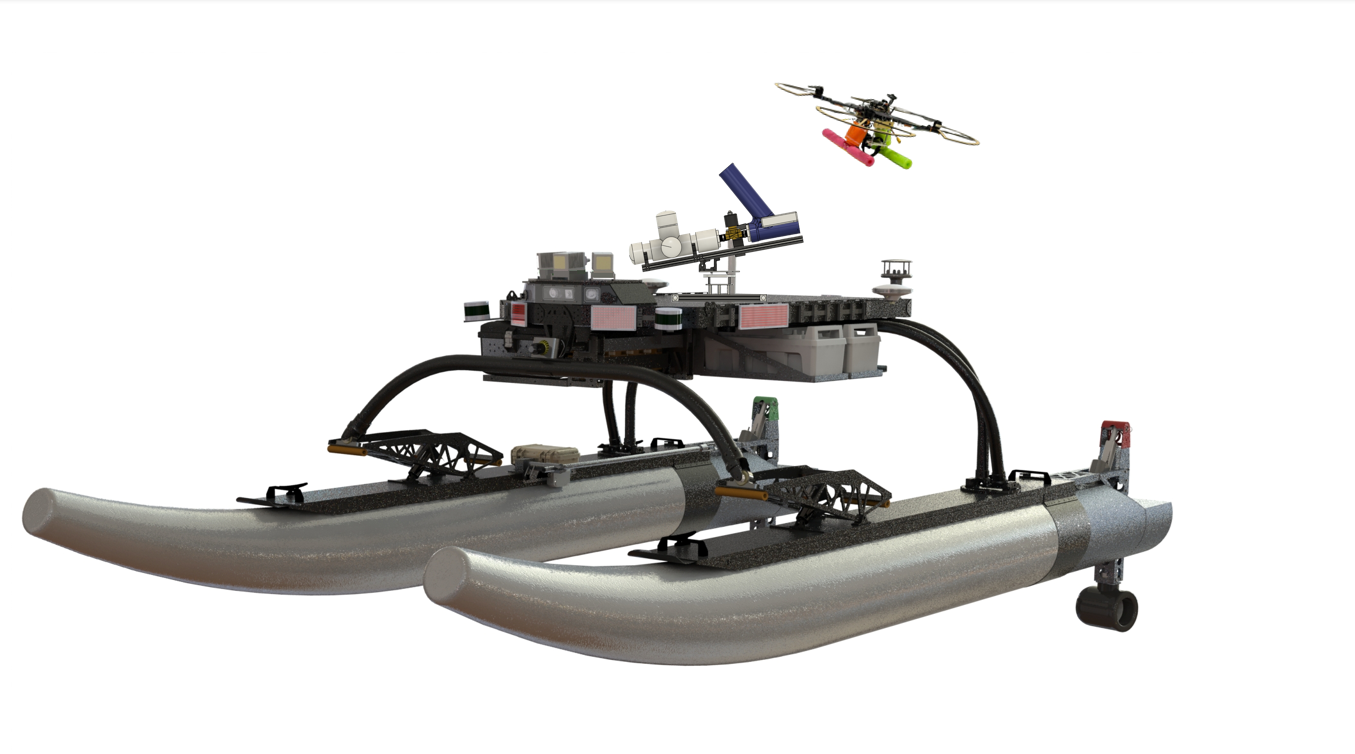
\includegraphics[width=0.8\textwidth]{Images/Minion.png}
\caption{ERAU's \ac{WAMV} Research Vessel Minion as configured for the 2024 Maritime RobotX Challenge.}
\label{fig:minion}
\end{figure}

The sensing configuration used in this research and the 2024 competition is described in Section \ref{perception_geometry}.
% The sensor configuration described in section \ref{perception_geometry} was originally developed by Team Minion for the 2022 and 2024 Maritime RobotX competitions \cite{holland2024, thompson2023}. 
Section~\ref{sensors} presents the technical specifications of Minion's sensor hardware, with particular emphasis on the \ac{LiDAR} and high-definition camera sensors selected for this study.
An overview of the CPU and network infrastructure of the system is provided in section~\ref{sec:Atlas_LAN} as background for the computational requirements of the real-time object detection methods presented in Chapter~\ref{realtime_object_detection}, as well as the challenges relating to the synchronization of sensors in section~\ref{sec:calibration}.
% housed within the forward camera enclosure. Section~\ref{visual_cameras} provides additional discussion regarding visual spectrum sensor selection and characterization. 
Of particular note, the timestamp embedding mechanism described in Section~\ref{time_sync_cam} overcomes network latency issues in the video pipeline to maintain a more precise temporal alignment.
% , essential for rigorous multi-modal sensor fusion analysis.
Finally, section~\ref{sensor_data} discusses the \ac{ROS} software architecture responsible for recording and processing sensor data.

%%%%%%%%%%%%%%%%%%%%%%%%%%%%%%%%%%%%%%%%%%%%%%%%%%%%%%%%%%%%%%%%%%%%
%%%%%%%%%%%%%%%%%%%%%%%%%%%%%%%%%%%%%%%%%%%%%%%%%%%%%%%%%%%%%%%%%%%%
\section{Perception Geometry} \label{perception_geometry}

Minion is equipped with six \ac{LiDAR} sensors as well as six cameras to perceive her surroundings.
Omnidirectional \ac{LiDAR} coverage is provided by three Velodyne VLP-16 units for situational awareness within the \acp{USV} immediate operating environment.
% \ac{LiDAR} coverage and object detection within the vessel's immediate operating environment.
Three additional forward-scanning Livox Horizon \ac{LiDAR} units generate a dense point cloud ahead of the vessel for object detection and classification at greater distances.
The Livox units are directly mounted to a camera enclosure which houses four high-definition visual-spectrum cameras and two \ac{LWIR} cameras.
The combination of forward-scanning LiDAR and cameras provides a significantly higher fidelity of data within a shared 165-degree \ac{FOV}. % in the direction of travel.
% The camera enclosure design emphasizes modularity and research flexibility.
Figure~\ref{fig:camera_enclosure} illustrates the mounting arrangement of the Livox Horizon LiDAR units and the six cameras within the waterproof enclosure.
Together, these sensors define the operational envelope of the perception system, encompassing a horizontal \ac{FOV} of approximately 160~degrees and an effective detection range of up to 60~meters.

\begin{figure}[htbp]
\centering
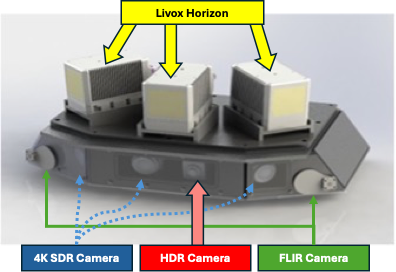
\includegraphics[width=0.6\textwidth]{Images/Camera_enclosure2.png}
\caption{Mounting locations of three Livox Horizon LiDAR units (yellow arrow, top), two LWIR cameras (green, thin, solid arrows), three FLIR 4k cameras (blue, dotted arrows), and a single \ac{HDR} camera  (red arrow, bottom) within the camera enclosure.}
\label{fig:camera_enclosure}
\end{figure}

% While the Velodyne \ac{LiDAR} sensors provide comprehensive 360-degree environmental awareness for navigation and collision avoidance, the three forward-facing Livox Horizon \ac{LiDAR} units mounted to the camera enclosure were selected for their superior point cloud density and ability to facilitate a higher resolution for object detection.
% The three Livox units concentrate sampling density in the forward \ac{FOV}, matching the horizontal coverage of the six cameras.
% Both modalities overlap the \ac{FOV} of their respective individual sensors.
% This sensor arrangement ensures higher density and more uniform point-cloud across the 165-degree forward perception envelope in the case of \ac{LiDAR}, but also makes the system more robust to failure.
% Losing a single sensor will not create a blind spot for either sensing modality in the forward path of motion of the \ac{USV}. 
% Figures~\ref{fig:fov_cam} and ~\ref{fig:fov_LiDAR} show how the horizontal \ac{FOV} for each of these sensors overlaps in the direction of travel.

% Each of these sensors is installed so that the center of their \ac{FOV} is parallel to one of three separate lines of vision.
% The first of these lines is a vector that points down the centerline of the vessel in the forward direction, and sensors in this orientation receive the moniker of \texttt{sensor\_center}.
% The other two lines of vision are rotated 40 degrees counterclockwise and clockwise from the centerline, and sensors in these orientations receive the moniker \texttt{sensor\_port} and \texttt{sensor\_starboard}, respectively.
Each sensor’s optical axis is aligned with one of three predefined sight lines: the vessel's centerline and two axes rotated $\pm 40$ degrees from the center.
% In the case of LiDAR, this sensor arrangement provides a denser point cloud and, in general, means that the loss of signal from any single sensor does not create a blind spot in the forward direction of travel.
For the LiDAR system, this configuration increases point-cloud density in the forward direction and ensures that loss of any single sensor does not produce a blind spot in the forward direction of travel.
% Figure~\ref{fig:fov_combined} shows the camera's \ac{FOV} in \ref{fig:fov_cam}, and the the LiDAR \ac{FOV} in \ref{fig:fov_LiDAR}.
Each of the three Livox Horizon LiDAR units has an 81.7-degree \ac{FOV}, resulting in more than a 40-degree overlap in the \ac{FOV} between \texttt{livox\_center} and both \texttt{livox\_port} and \texttt{livox\_starboard}, and approximately 3 degrees of overlap between \texttt{livox\_port} and \texttt{livox\_starboard} (figure~\ref{fig:fov_LiDAR}).
Three 4K cameras are configured to point in along each of these three sight lines. 
While these cameras are equipped with a Theia-TL410P zoom lens, they are currently set at a fixed zoom level that approximates a 65-degree horizontal \ac{FOV}, which provides a 15-degree overlap in their \ac{FOV} (figure~\ref{fig:fov_cam}).
The two \ac{LWIR} cameras each have a 90-degree \acs{FOV}, and are positioned along the port and starboard vision lines, providing a 10-degree overlap.
Finally, there is a single HDR camera with a 65-degree horizontal \ac{FOV} that points forward.
While the \ac{HDR} camera lacks any of the aforementioned sensor redundancy, its \ac{FOV} aligns with the central 4k camera and was added for research that compared the two center-line mounted cameras \cite{liebergall}.

% related to the dynamic range of the two center-line mounted cameras  and was selected as the primary visual range sensor for this body of work for reasons that are discussed in section~\ref{visual_cameras}.


\begin{figure}[htbp]
\centering
\begin{subfigure}[t]{0.48\textwidth}
    \centering
    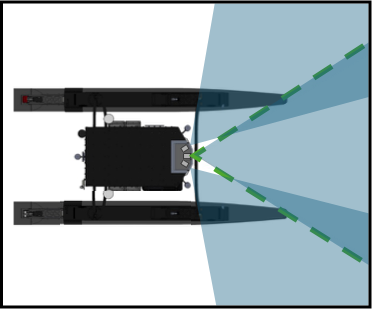
\includegraphics[width=\textwidth]{Images/fov_cam.png}
    \caption{Blue cones represent \ac{FOV} from individual FLIR 4K camera; green dashed lines indicate \ac{FOV} of HDR camera.}
    \label{fig:fov_cam}
\end{subfigure}
\hfill
\begin{subfigure}[t]{0.48\textwidth}
    \centering
    \includegraphics[width=\textwidth]{Images/fov_LiDAR.png}
    \caption{LiDAR horizontal \ac{FOV} overlap.}
    \label{fig:fov_LiDAR}
\end{subfigure}
\caption{Comparative visualization of horizontal \ac{FOV} (FOV) overlap for (a) cameras and (b) LiDAR sensors.}
\label{fig:fov_combined}
\end{figure}

% A Torc Robotics PinPoint \ac{GPS}/\ac{IMU} system is equipped with provides both global time synchronization and platform pose estimation.

% The sensor coordinate frames are organized in a hierarchical transformation tree structure, which is shown in \ref{transform_diagm}.
% The inertial reference frame (\texttt{map}) defines the world-fixed coordinate system.
% The platform reference frame (\texttt{base\_link}) represents the vessel body frame defined by the PinPoint \ac{GPS}/\ac{IMU}.
% The center Livox frame (\texttt{livox\_center}) serves as the primary sensor reference frame, with \texttt{livox\_port} and \texttt{livox\_starboard} both reporting data in the \texttt{livox\_center} reference frame.
% Six camera image frames exist within this tree, and are referenced to the \texttt{livox\_center} frame.
% Intrinsic calibration parameters, including camera-specific matrices and distortion coefficients, along with extrinsic transformation parameters relating sensor frames to each other and to the platform frame, are discussed in \textcolor{red}{Appendix \#}.

% The Livox scan pattern employs a non-repetitive rosette pattern that progressively covers the \ac{FOV} over time rather than repeatedly sampling fixed positions.
% This characteristic enables temporal aggregation to increase effective spatial resolution, particularly beneficial for a moving platform where \ac{GPS}/\ac{IMU} pose data enables motion-compensated point cloud accumulation.

% The dual \ac{LiDAR} architecture serves complementary purposes.
% The Velodyne VLP-16 units provide the omnidirectional awareness required for autonomous navigation, while the Livox Horizon sensors optimize point cloud density specifically within the forward camera \ac{FOV} for fusion research.
% The onboard This configuration enables comparative evaluation of detection performance while maintaining operational navigation capabilities.
% The sensor suite supports the research objectives of comparing detection performance across modalities and evaluating late fusion approaches.
% The following subsections detail individual sensor specifications and selection rationale.

% The primary sensors used for the data collected for this research were from the forward-facing perception module, referred to as the camera enclosure.

%%%%%%%%%%%%%%%%%%%%%%%%%%%%%%%%%%%%%%%%%%%%%%%%%%%%%%%%%%%%%%%%%%%%
%%%%%%%%%%%%%%%%%%%%%%%%%%%%%%%%%%%%%%%%%%%%%%%%%%%%%%%%%%%%%%%%%%%%
\section{Sensors} \label{sensors}

% The Minion platform integrates multiple sensor modalities to support maritime perception research.
% This section details the specifications and characteristics of the visual cameras (Section~\ref{visual_cameras}) \ac{LiDAR} systems (Section~\ref{sensors_LiDAR}), and navigation sensors (Section~\ref{gps_ins}) used in this research.
% , thermal cameras (Section~\ref{thermal_cameras}), and navigation sensors (Section~\ref{gps_ins}) 

%%%%%%%%%%%%%%%%%%%%%%%%%%%%%%%%%%%%%%%%%%%%%%%%%%%%%%%%%%%%%%%%%%%%
\subsection{LiDAR} \label{sensors_LiDAR}

% The Minion platform features six \ac{LiDAR} units providing both omnidirectional environmental awareness and forward-facing high-density perception.
% The \ac{LiDAR} suite is comprised of three Velodyne VLP-16 pucks and three Livox Horizon units.

% Three Velodyne VLP-16 \ac{LiDAR} sensors are positioned at aft-center, with the other two placed at approximately one-third intervals around the vessel at forward-port and forward-starboard, providing complete 360-degree coverage for navigation as well as object detection and avoidance.
% An additional three Livox Horizon solid-state forward-scanning \ac{LiDAR} sensors provide high-density measurements within the forward direction of motion.
Three Velodyne VLP-16 \ac{LiDAR} sensors are installed around the vessel to provide omnidirectional situational awareness. 
One unit is mounted near the aft-center position, and the other two are positioned at approximately one-third intervals around the forward-port and forward-starboard quadrants. 
Together, these sensors deliver nearly continuous 360° coverage for navigation and obstacle avoidance.

Each VLP-16 employs 16 lasers arranged in a vertical array that scans 16 distinct points elevation over its 30-degree vertical \ac{FOV} continuously over the 360-degree azimuth, producing approximately 300,000 \ac{pps} in single-return mode. 
The units are installed with a downward declination of approximately 5 degrees from the plane of the \ac{USV} deck to minimize blind-spots near the vessel's waterline.
As a result, one-half to one-third of their scanning azimuth is well above the horizon or pointing directly into the vessel and is discarded, drastically reducing the number of points each unit can publish.

% Both of these units are capable of approximately 1.4 million measurements per second.
% For an equivalent 80-degree horizontal FOV, the Velodyne’s effective $317,700 \text{ pts/sec}$ represents $\approx 22 \%$ of the overlapping \ac{FOV} of the Livox unit’s output.
% % While each Velodyne VLP-16 unit is capable of producing 300k \ac{pps} compared to the Livox unit's 280k, their 360-degree scanning pattern means that only 
% The principal distinction between them lies in their underlying scanning architectures and sampling density, which directly influences perception fidelity.
% The Velodyne VLP-16 LiDAR scans 16 discrete points spanning a 30-degree vertical \ac{FOV} emanating from the azimuthal plane of the device in a 360-degree horizontal \ac{FOV}that repeats identically with each rotation. 
% The points generated span the 360
% % To minimize blind spots near the base of Minion, each of the Velodyne units is mounted at a 15-degree declination from the vessel's deck plane, resulting in 
% These rings are notF
% % For vessels moving at typical speeds (2-5 m/s), platform displacement between rotations remains small relative to object size, resulting in near-perfect overlap of consecutive scans.
% At typical vessel speeds between $2 \text{to} 5 m/s$, successive Velodyne rotations overlap almost perfectly, causing sparse sampling of small or distant targets.
% % This means that small to medium-sized objects may not even be detected when at large distances from the sensor, as illustrated in Figure \ref{fig:LiDAR_scan_compare}.
% Consequently, small or distant targets may be undersampled or entirely missed in sequential Velodyne frames (Figure \ref{fig:LiDAR_scan_compare}).

In contrast, the three Livox Horizon solid-state \ac{LiDAR} units concentrate their scanning pattern within an $81.7 \times 25.1$ degree \ac{FOV}, generating up to 280,000 \ac{pps}. 
Although the nominal point rates are comparable, the Livox pattern can return $100 \%$ of its concentrated \ac{FOV} data. 
This higher spatial sampling density enables detection and classification of objects that may be smaller or further from the sensor.
A direct comparison of the discrepancy between the Velodyne and Livox scan patterns and point density is provided in Figure \ref{fig:LiDAR_scan_compare}.
The top-right image shows the dense point cloud of the Livox devices.
The light tower in the foreground and the large dock structure in the background can be seen in the camera view (left) and are both well defined in the red point cloud.
Two small buoys are also distinctly visible between the two structures.
In comparison, the point cloud returned by the Velodyne devices is shown in the bottom-right. 
The general form of the light tower can be seen; however, there are very few points returned from the large dock structure in the background, and the round buoys are undetected.

% The forward-scanning Livox devices operate differently, tracing a non-repetitive pattern across the \ac{FOV}.
% Two orthogonal mirrors oscillate at slightly different frequencies to cause the laser beam to trace a path that progressively fills the \ac{FOV} without repetition as shown in Figure ~\ref{fig:livox_scan_pattern}.

\begin{figure}[htbp]
\centering
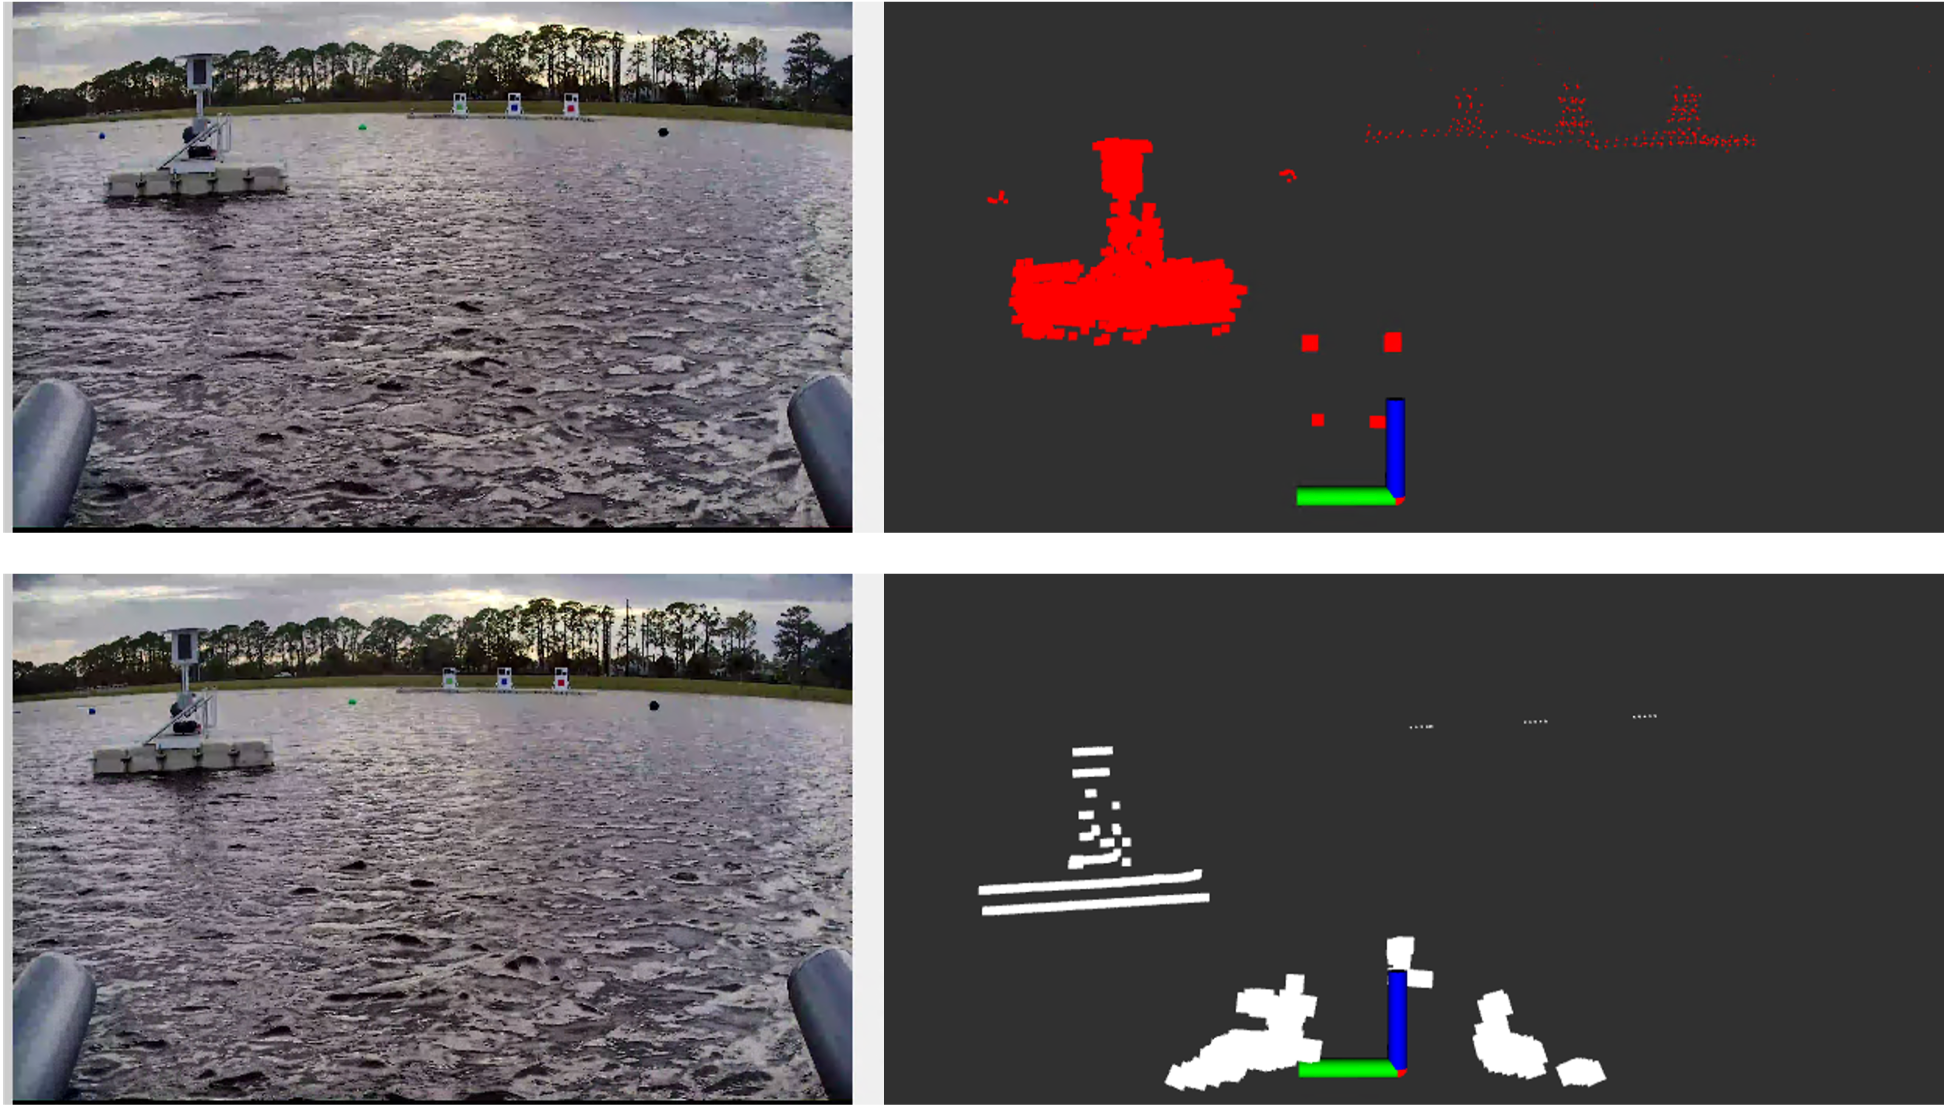
\includegraphics[width=0.8\textwidth]{Images/LiDAR_compare.png}
\caption{A comparison of LiDAR returns from the Livox units (top-right, red) and Velodyne units (bottom-right, white) to the respective HDR camera view (top-left and bottom-left). LiDAR points are viewed from third-person point of view in RVIZ. Green and Blue axes (top-right, top-bottom) represent the origin of the USV frame of reference.}
\label{fig:LiDAR_scan_compare}
\end{figure}

% The superior point density of the overlapping forward-scanning  LiDAR is critical for the real-time object detection method that is discussed in \textcolor{red}{Section \#}.
% The overlapping forward-scanning LiDAR provides the spatial density required for the real-time object-detection framework described in Section \ref{gbcache}.
% For this reason, the research presented in this work exclusively utilizes LiDAR data from the Livox Horizon sensors.

Consequently, the research presented in this work relies exclusively on LiDAR data from the forward-scanning Livox Horizon sensors, whose concentrated and non-repetitive coverage provides the spatial resolution required for the real-time object-detection framework described in Section \ref{gbcache}.
        %%%%%%%%%%%%%%%%%%%%%%%%%%%%%%%%%%%%%%%%%%%%%%%%%%%%%%%%%%%%
\subsubsection{Livox Horizon} \label{sensors_livox}

% Each Livox Horizon employs two orthogonal mirrors operating at different frequencies to trace a complex Lissajous-like path that progressively fills the $81.7 \times 25.1$-degree (horizontal × vertical) \ac{FOV}, as illustrated in Figure~\ref{fig:livox_scan_pattern}. 
% The three Livox units are mounted with 40 degrees of horizontal separation, overlapping each other \ac{FOV} by $\approx 50\%$, making the system robust to failure of any single unit, as well as effectively doubling the rate of sampled points and distributing them more evenly across the center device's \ac{FOV}. 
Each Livox Horizon uses dual orthogonal mirrors oscillating at slightly different frequencies to generate a non-repetitive Lissajous-like scan pattern over its $81.7 \times 25.1$ degree \ac{FOV}. 
Overlapping these sensors by roughly $50 \%$ effectively doubles the point density along the center-line path under nominal operation, and maintains coverage under single-unit failure.
Table~\ref{table:livox_horizon_specs} presents detailed hardware specifications for the Livox Horizon.

% The rosette scan pattern is provided in \ref{fig:livox_scan_pattern}, and table \ref{table:livox_horizon_specs} presents the Livox Horizon specifications.

\begin{figure}[htbp]
\centering
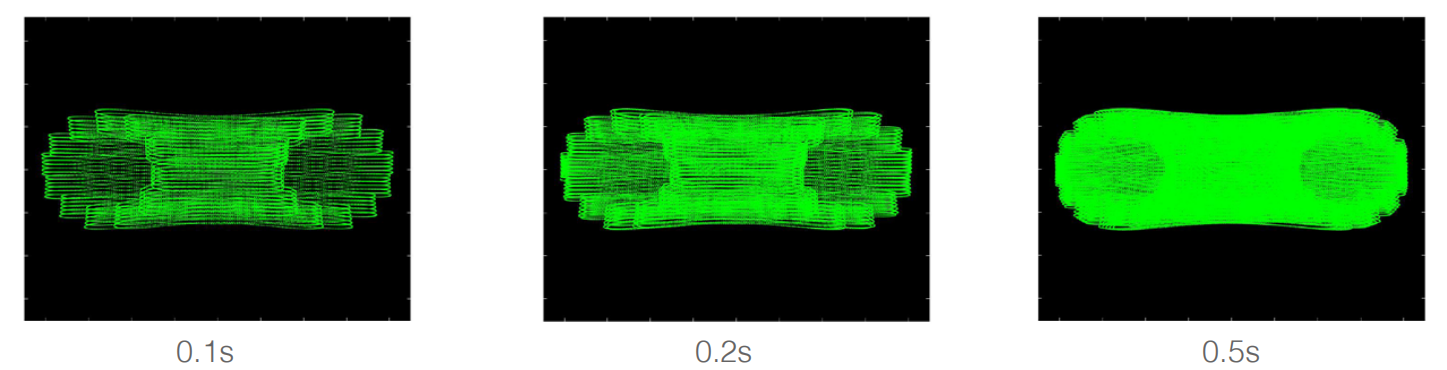
\includegraphics[width=0.8\textwidth]{Images/Livox_1.png}
\caption{Accumulation of points with the Livox Horizon's non-repetitive scan pattern, from 0.1 to 0.5 seconds  \cite{livox_manual}.}
\label{fig:livox_scan_pattern}
\end{figure}

Each device is capable of returning up to $4.8 \times 10^5$ \ac{pps} in dual return mode, with each return consisting of position coordinates (x, y, z), target reflectivity, and timestamp.
This operational mode returns two data points for each laser emission and is useful for situations where the sensor scans semi-permeable objects such as windows, thick tree canopies, or water.
% Instead, each device is operated in single-return mode for two reasons.
% The first is a consideration of available network bandwidth.
Each sensor operates in single-return mode, primarily to reduce network load.
A conservative estimate of 16 bytes per point results in $\approx 23 \text{ Mbps}$ which would quickly overwhelm the \ac{USV}'s network.
% Luckily, the 905 nm near-infrared wavelength of the emitted laser experiences strong absorption by water. 
However, The $905 nm$ near-infrared emission is strongly absorbed by water, effectively suppressing subsurface returns.
This means that only points which are reflected by the water surface are returned with an intensity greater than zero, making it straight forward to filter out points in the ground plane.

\begin{table}[htpb]
\centering
\begin{tabular}{ll}
\hline
\multicolumn{2}{c}{Livox Horizon}\\
\hline
% \textbf{Parameter} & \textbf{Value} \\
\hline
Model & Livox Horizon \\
Horizontal Field of View & 81.7 degree \\
Vertical Field of View & 25.1 degree \\
Range & 260 m @ 80\% reflectivity \\
Point Rate (Single Return) & 240,000 pts/sec \\
Point Rate (Dual Return) & 480,000 pts/sec \\
Range Precision & ±2 cm \\
Wavelength & 905 nm \\
Scan Pattern & Non-repetitive rosette \\
Interface & Ethernet \\
Operating Frequency & 100 Hz \\
\hline
\end{tabular}
\caption{LiDAR Specifications}
\label{table:livox_horizon_specs}
\end{table}


%%%%%%% move to sensor calibration %%%%%%%%%%%
% Accurate fusion of data from multiple \ac{LiDAR} units requires precise knowledge of sensor geometric relationships.
% The Livox Horizon units feature onboard storage for extrinsic calibration parameters, enabling each sensor to transform its measurements to a common reference frame before transmission.
% These parameters are written to non-volatile memory on each Livox unit and applied before data transmission so that all LiDAR returns are received in the center \ac{LiDAR}'s reference frame, reducing the necessary calculation further down the data pipeline.
% \textcolor{red}{cite Livox documentation?}.
% enhancing their real-time operational advantage by reducing additional computation later in the pipeline.
% The calibration methodology to determine these extrinsic values is detailed in Section~\ref{LiDAR_extrinsic}.
%%%%%%%%%%%%%%%%%%%%%%%%%%%%%%%%%%%%%%%%%%%%%%%

% The 905 nm near-infrared wavelength experiences strong absorption by water, resulting in minimal returns from water surfaces.
% This characteristic benefits maritime object detection by reducing clutter from waves that would otherwise trigger false positives in clustering algorithms.

% The fundamental distinction between the Livox Horizon and traditional spinning \ac{LiDAR} lies in the scan pattern.
% A mechanically spinning sensor with N lasers produces N discrete horizontal rings that repeat identically each rotation.
% For vessels moving at typical speeds (2-5 m/s), platform displacement between rotations remains small relative to object size, resulting in near-perfect overlap of consecutive scans.
% The Livox operates differently, employing a two-dimensional scanning mechanism that traces a non-repetitive rosette pattern across the \ac{FOV}.
% Two orthogonal mirrors operating at slightly different frequencies cause the laser beam to trace a complex Lissajous-like path that progressively fills the \ac{FOV} without repetition \cite{thompson2023}.

% Scan pattern coverage accumulates over time, with longer integration periods yielding denser spatial sampling.
% At the standard 100 Hz output rate, each \ac{UDP} message contains approximately 10 milliseconds of returns.
% Over a one-second aggregation period, the rosette pattern provides substantially higher spatial coverage than a spinning sensor's fixed ring geometry.

% The non-repetitive forward-scanning nature of the Livox units means that point cloud density is not uniform across the \ac{FOV}.
% The 81.7-degree horizontal \ac{FOV} allows for overlap between the three units, achieving more uniform density across the 165-degree \ac{FOV}, matching the 4K FLIR camera coverage.

% Insert figure showing Livox scan pattern here
% \begin{figure}[htbp]
% \centering
% 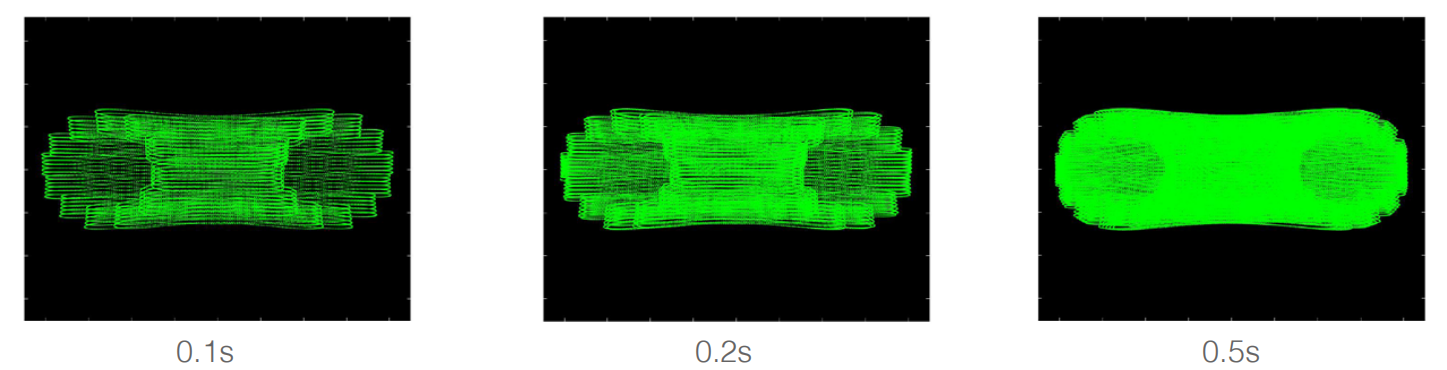
\includegraphics[width=0.8\textwidth]{Images/Livox_1.png}
% \caption{Livox Horizon non-repetitive rosette scan pattern demonstrating point cloud density distribution from 0.1 to 0.5 seconds.}
% \label{fig:livox_scan_pattern}
% \end{figure}




% A Velodyne VLP-16 in dual-return mode produces approximately 1.4 million \ac{pps} distributed across the full 360-degree plane.
% The camera \ac{FOV} encompasses approximately 165 degrees, yielding an effective point rate in the region of interest of:

% $$\text{Effective HDL-32E rate} = 1.4 \times 10^6 \times \frac{165 degree}{360 degree} \approx 641,000 \text{ pts/sec}$$

% Three Livox Horizon units in dual-return mode together produce:

% $$\text{Combined Livox rate} = 3 \times 480,000 = 1.44 \times 10^6 \text{ pts/sec}$$

% This represents a 2.25× increase in point returns within the camera view, excluding additional benefits from superior vertical sampling achieved through the non-repetitive pattern compared to fixed 32-ring geometry \cite{thompson2023}.

%%%%%%%%%%%%%%%%%%%%%%%%%%%%%%%%%%%%%%%%%%%%%%%%%%%%%%%%%%%%%%%%%%%%
\subsection{Visible Spectrum Cameras} \label{visual_cameras}

% \textcolor{red}{Expand this entire discussion}
% The visible spectrum camera suite on the Minion platform is designed to balance two factors that are particularly important for maritime perception: imaging resolution and dynamic range.

For computer vision and perception tasks, system performance is directly influenced by the quality of the visual input.
The fidelity of an image is determined by a camera's hardware and integrated software; therefore, camera selection is a critical design consideration in any vision-based system. 
Sensor size and lens characteristics determine the spatial detail captured, while shutter speed, exposure, and onboard processing influence brightness, contrast, and color balance. 
The visible-spectrum cameras housed within the camera enclosure were selected to balance image resolution and dynamic range, two essential factors for reliable maritime perception.
A brief discussion of both of these metrics is presented here to justify utilizing data acquired from the \ac{HDR} camera for this research.

\subsubsection{Image Resolution}
Camera resolution determines the ability to resolve small targets at a distance.
% , and appropriate imaging sensors and lenses can be selected by determining the maximum distance and minimum size at which objects need to be resolved.
% Camera resolution dictates the minimum discernible target size at range; lens and sensor parameters are therefore chosen to meet specified detection distances.
% Camera resolution governs the minimum resolvable target size; lens and sensor parameters are thus selected to ensure detection at required ranges.
To ensure adequate perception across the operational envelope, cameras must resolve objects to a required minimum resolution when the object is at the maximum detection range.
% The resolution of an object in the image frame can be determined if the object's width $\mathit{l}$ and distance from the camera $d$ are knownwith
The relationship between an object's physical width $\mathit{w}_{obj}$ and pixel width within an image $\mathit{w}_{\text{px}}$ is given by
% Provided a maximum detection range $d$ and the width of the smallest object to be detected $W$, the camera's focal length and resolution requirements can be determined by assuming a pinhole-camera model \cite{matlab_calibration}, can be derived as:
% we can determine the necessary optical focal length and resolution for the sensor.
% For an object of physical width $W$ at distance $d$, its width in the image frame $w_{\text{px}}$ is approximated by

\begin{equation}
\mathit{w}_{\text{px}} = f \; \frac{N_x}{S_w}\frac{\mathit{w}_{obj}}{d}
\end{equation}

% where $\mathit{l}_{\text{px}}$ is the pixel width of an object in the image frame, 
where $f$ is the \ac{EFL} of the camera and lens, $N_x$ is the horizontal image resolution in pixels, and $S_w$ is the width of the image sensor.
% This equation is used for sensor selection by determining the minimum resolution required for the smallest object to be detected at the maximum detection range.
This equation can be used to determine camera requirements if the true size of the imaged objects is known, or to determine a reasonable expectation of object resolution if the camera values are known.
This relationship is also critical for determining the distortion present in each camera/lens system, detailed further in section~\ref{spatial_calibration}.

Defining the requirement for the minimum resolution of an object in the image frame requires an understanding of the object detection method used with visual cameras, as well as the objects being detected. both of which will be discussed in greater detail in sections ~\ref{dataset} and ~\ref{yolo}, respectively.
% For now, it is sufficient to know that the smallest object we wish to detect is $0.3683$ meters wide at a distance of 60 meters.
% , and that we have optical and digital resolution requirements to consider.
This image detection architecture is discussed in section ~\ref{yolo}.
For camera selection, it is sufficient to know that this method scales down each input image to a resolution of $640 \times 640$ pixels for processing efficiency.
This should be considered when defining the minimum pixel density of a camera's sensor, as it alters our prior equation slightly.

\begin{equation}
\mathit{w}'_{\text{px}} = f \; \frac{640 \text{px}}{S_w}\frac{\mathit{w}_{obj}}{d}
\end{equation}
% This means that an image captured at $4000 \times 3000$ pixels is reduced to $650 \times 487$ pixels, which is $16.25\%$ of its original size.
% As an example, if the text on waterway signage 60 meters away is legible at a resolution of 100 pixels wide in a 1,000 $\times$ 1,000 pixel image, it would need a resolution of 162 pixels to meet the additional requirements imposed by the image detection algorithm.
Each camera within the enclosure was selected using these metrics, and object information based on the obstacles commonly associated with the RobotX Maritime Challenge. %, in addition to other contemporaneous research \cite{thompson2023} \textcolor{red}{(check scholarly commons)}.

% \textcolor{red}{add back: ?}
Given that the smallest object we wish to detect is $0.3683$ meters wide at a distance of 60 meters.
The two visual spectrum camera models within the camera enclosure have a similar focal length, and resolutions of $4000 \times 3000$ px and $2880 \times 1860$ px. Examining the camera with the smaller horizontal resolution of 1880 px (which has a sensor width of $S_{w} = 8.64$ mm), we obtain the width of our object in the image frame as
% meet this requirement; the object detection method used will impose a secondary constraint.
\begin{equation*}
\begin{split}
    \mathit{w}_{\text{px}} & = 8\;\text{mm} \cdot \frac{2880\;\text{px}}{8.64\;\text{mm}} \cdot \frac{0.3683\;\text{m}}{60\;\text{m}}\\
     & = 16.36 \approx 16 \;\text{px}
\end{split}
\end{equation*}

With the additional scaling required by the visual object detection method, the minimum width of our object becomes 
\begin{equation*}
\begin{split}
    \mathit{w}'_{\text{px}} & = 16\;\text{px} \cdot \frac{640\;\text{px}}{2880\;\text{px}} \\
     & = 3.\overline{55} \approx 3 \;\text{px}
\end{split}
\end{equation*}

Figure \ref{fig:A2_multi_res} shows our smallest object, Polyform A2 round buoy, at a selection of resolutions, and is still recognizable at a resolution of 16 pixels wide. %, and becomes less defined at lower resolutions. 
This operation is repeated to predict the width of the object in the image frame at a range of distances up to our maximum of 60 meters, and the results are provided in Table \ref{table:buoy_res}.
From this information, the buoy will be easily recognizable at any range by visual inspection, but will become much less defined when the image is scaled down for the visual object detection method.
As we will discuss in section \ref{yolo}, this method may struggle to detect this size buoy at distances greater than 20 meters.

\begin{table}[htpb]
\centering
\begin{tabular}{c|c|c}
\hline
\multicolumn{3}{c}{Polyform A2 Buoy Resolution at Range}\\
\hline
% \textbf{Parameter} & \textbf{Value} \\
\hline
Object Distance & Image Frame Width & With Detection \\
\hline
10 m & 98 px & 21 px \\
20 m & 49 px & 10 px \\
30 m & 32 px & 7 px \\
40 m & 24 px & 5 px \\
50 m & 19 px & 4 px \\
60 m & 16 px & 3 px \\
\hline
\end{tabular}
\caption{The predicted resolution of a $\mathit{l} = 0.3683$ meter wide object within the Loepard Imaging HDR camera's image frame at multiple distances.}
\label{table:buoy_res}
\end{table}

\begin{figure}[htbp]
\centering
\begin{subfigure}[t]{0.245\textwidth}
    \centering
    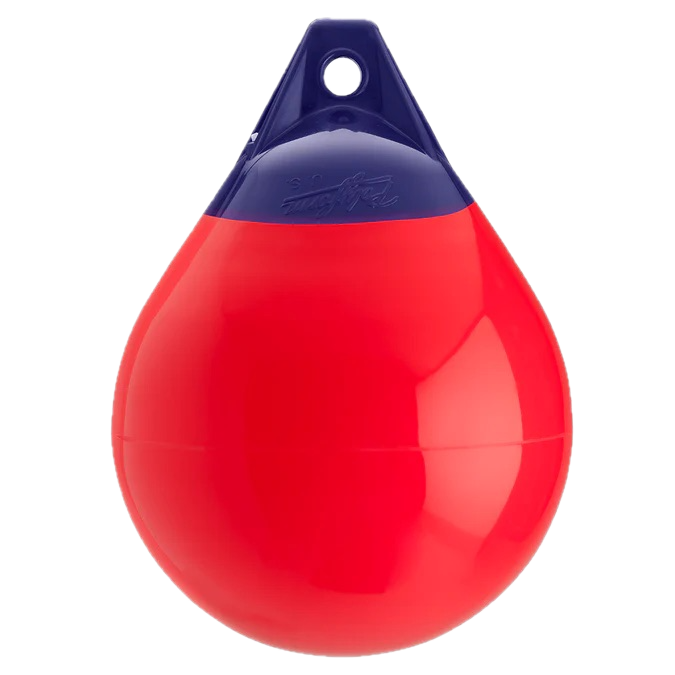
\includegraphics[width=\textwidth]{Images/A2.png}
    \caption{\raggedright{Polyform A2 Buoy}}
    \label{fig:A2}
\end{subfigure}
\hfill
\begin{subfigure}[t]{0.245\textwidth}
    \centering
    
\includegraphics[width=\textwidth]{Images/A2_16px.png}
    \caption{
    16 pixel width,\\  
    % $\approx$ 60 m with HDR
    }
    \label{fig:A2_16px}
\end{subfigure}
\hfill
\begin{subfigure}[t]{0.245\textwidth}
    \centering
    
\includegraphics[width=\textwidth]{Images/A2_6px.png}
    \caption{
    6 pixel width,\\  
    % $\approx$ 40 m with HDR \\ 
    % \& object detection.
    }
    \label{fig:A2_6px}
\end{subfigure}
\hfill
\begin{subfigure}[t]{0.245\textwidth}
    \centering
    
\includegraphics[width=\textwidth]{Images/A2_3px.png}
    \caption{
    3 pixel width,\\  
    % $\approx$ 60 m with HDR \\ 
    % \& object detection.
    }
    \label{fig:A2_3px}
\end{subfigure}
\caption{Polyform A2 Buoy (a), visualized at 16 pixels (b), 6 pixels (c), and 3 pixels wide (d).}
\label{fig:A2_multi_res}
\end{figure}


% Insert equation to get the horizontal focal length / horizontal resolution ratio needed for camera selection based upon the equation and information provided above
% Assuming our camera will have a landscape aspect ratio, our equation becomes 
% Since the detection network downsamples each input frame to a maximum dimension of 640 pixels while preserving aspect ratio, a landscape-oriented image with native resolution $N_x \times N_y$ (where $N_x > N_y$) is scaled such that the horizontal dimension becomes 640 pixels.
% For an object that must occupy at least $w_{\text{net}}$ pixels horizontally in the network input to be reliably detected, the camera system must satisfy
%   \begin{equation}
%   \frac{f}{S_w} = \frac{w_{\text{net}} \, d}{640 \, W}
%   \end{equation}
% \begin{equation}
%  w_{\text{px}} \left(\frac{650}{N_x}\right) = f \; \frac{N_x}{S_w}\frac{W}{d}
% \end{equation}

% where the ratio $f/S_w$ represents the normalized focal length of the camera-lens system.
% Substituting the minimum object dimensions ($W = 0.3683$ m, $d = 60$ m) and assuming a minimum network resolution requirement of $w_{\text{net}}$ pixels, this relationship defines the optical design space for camera selection.
% This makes our equation

% \begin{equation}
% w_{\text{px}} = \frac{f \, N_x^2 \, W}{(680)S_w \, d}
% \end{equation}



% The dynamic range of an imaging sensor refers to the range of signal intensities it can detect, and can be as critical as image resolution when selecting camera sensors.
\subsubsection{Dynamic Range}
Dynamic range describes the ratio between the brightest and darkest signal levels a camera sensor can record.
Light levels that exceed the camera sensor's range cause the image to appear white or "blown-out", while light levels that are too low will appear darker, with detail being indistinguishable from noise.
% Dynamic range—the span of detectable signal intensities—is equally critical to sensor selection as spatial resolution.
\acp{USV} and \acp{AGS} routinely operate in environments where bright sky reflections and deep shadows are common, often within the same scene.
Therefore, selecting a camera with insufficient dynamic range may lead to washed-out highlights or lost detail in shadows.

Dynamic range, expressed in dB, is given by
\begin{equation}
 \text{Dynamic Range (dB)} = 20 \log{\left( \frac{N_{sat}}{N_{noise}}\right) }
\end{equation}
where $N_{sat}/N_{noise}$ is the ratio of the saturation to the minimum signal a camera sensor can detect above background noise.
% Higher dynamic range can be achieved through software by combining sequential multi-exposure images, or through a digital overlap \ac{HDR} (DOL-HDR) architecture with in-pixel dual conversion gain.
% Sequential multi-exposure \ac{HDR}, which stacks separate frames and is prone to ghosting or blurring, therefore 
% DOL-\ac{HDR} is preferred when precise synchronization of the imagery is required, such as sensor fusion.
% Because maritime environments routinely present both bright sky reflections and deep shadows in the same scene, dynamic range is as critical as resolution when selecting cameras for perception tasks. 
High-dynamic-range (HDR) imaging can be achieved in two primary ways. 
The first is sequential multi-exposure \ac{HDR}, in which multiple frames captured at different exposure settings are combined to extend the tonal range \cite{Reinhard2010}. An example is provided in Figure \ref{fig:hdr_example}.



While effective for static scenes, this approach introduces motion-related artifacts such as ghosting and motion-blur as the relative velocity increases between the sensor and objects within the frame.
The second method uses an in-sensor technique called dual-conversion gain (DCG) that combines multiple light exposure levels within a single frame of exposure. 
% \textcolor{red}{Coyle: It isn't short and long exposure, but changing the size of the exposure pixel to capture more/less light from my understanding. This is why it doesn't motion blur} By capturing short and long exposure data within a single frame, this method avoids the distortion of multi-exposure \ac{HDR}.
The two visible sensing technologies considered for this research are described below.

\begin{figure}[htbp]
    \centering
    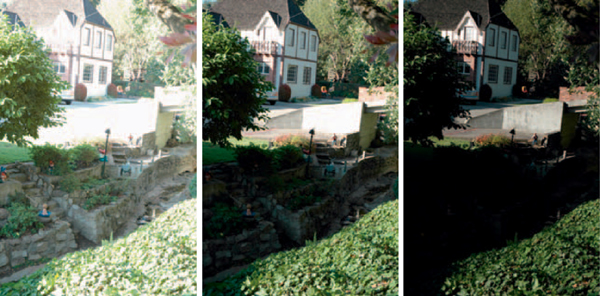
\includegraphics[width=0.65\linewidth]{Images/hdr_example.png}
    \caption{An example of multi-exposure HDR frame-stacking \cite{Reinhard2010}.}
    \label{fig:hdr_example}
\end{figure}
%%%%%%%%%%%%%%%%%%%%%%%%%%%%%%%%%%%%%%%%%%%%%%%%%%%%%%%%%%%%%%%%%%%%
\subsubsection{FLIR Blackfly S 4K Cameras} \label{sensors_FLIR}

% Three FLIR Blackfly S 4K visible-light cameras, arranged to provide a combined 165 degrees of forward-facing coverage through overlapping 65-degree lenses.  
Three FLIR Blackfly S 4K cameras are aligned to the port, center, and starboard sight-lines described in section \ref{perception_geometry} to provide a combined 165-degree horizontal \ac{FOV}.
In addition to redundancy, this configuration avoids additional spherical distortion within the image that would be required to cover the same \ac{FOV} with fewer cameras.
% Each camera is paired with a Theia TL410P zoom lens with an \ac{EFL} of \textcolor{red}{???} and an image resolution of $4096 \times 4096$, ensuring that objects remain adequately resolved across the vessel's perception envelope.  
Each FLIR Blackfly has a resolution of 4096 $\times$ 4096 pixel resolution and is paired with a Theia TL410P zoom lens at a fixed \ac{EFL} $\approx$ 8 mm.
% This sensor dimension and \ac{EFL} exceeds the pixel density required to ensure object resolution across the operational envelope.


\begin{table}[htbp]
\centering
\begin{tabular}{ll}
\hline
\multicolumn{2}{c}{FLIR 4K SDR Camera}\\
% HDR & Camera\\
\hline
% \textbf{Parameter} & \textbf{Value} \\
\hline
\multicolumn{2}{c}{Camera Sensor}\\
\hline
FLIR & Blackfly S 120S4C \\
% Image Sensor & Sony IMX490 \\
% Pixel Size & $3.0 \times 3.0 \mu m$ \\
Horizontal Resolution & 4000 pixels \\
Vertical Resolution & 3000 pixels \\
Aspect Ratio & 1.33:1 \\
Maximum Frame Rate & 31 fps \\
Dynamic Range & 69.4 dB \\
\multicolumn{2}{c}{Camera Lens}\\
\hline
Theia & TL410P\\
% Aperture F/\# & $2.0$ \\
Horizontal \Ac{FOV} & 65-degrees\\
Lens \Ac{EFL} & approx. 8 mm\\
% Vertical Field of View & 37 degrees \\
\hline
\end{tabular}
\caption{FLIR 4K SDR Camera Specifications}
\label{table:SDR_camera_specs}
\end{table}

The Blackfly S sensor captures video at 31 \ac{fps} and achieves a dynamic range of 69.4 dB, which is within the \ac{SDR}.
% This corresponds to a span of a few thousand-to-one between the darkest detectable signal and the brightest non-saturating signal.  
% The cameras capture 31 \ac{FPS} at a resolution of 4096 $\times$ 2160 pixels.
% \textcolor{red}{Add discussion of pixel density sensor selection in the context of the requirement to resolve specific objects at a minimum resolution at a maximum specific distance. This will require equations.}

%%%%%%%%%%%%%%%%%%%%%%%%%%%%%%%%%%%%%%%%%%%%%%%%%%%%%%%%%%%%%%%%%%%%
\subsubsection{Leopard Imaging HDR Camera} \label{sensors_HDR}

% A Leopard Imaging LI-USB30-IMX490-GW5400-GMSL2-065H camera, based on Sony’s IMX490 automotive-grade \ac{HDR} sensor, provides 65-degree of forward \ac{FOV}.  
The Leopard Imaging camera provides a 65-degree forward \ac{FOV} using Sony’s automotive-grade IMX490 sensor with 120 dB of dynamic range.
The \ac{HDR} is achieved via Sony’s \ac{DOL-HDR} architecture, which combines large and small photodiodes within each pixel on the sensor.
Each size of sub-pixels experience a different photon flux during each frame of exposure, and each output is read at both high and low conversion gains.
This method yields 4 measurements of light intensity within each captured frame, eliminating motion artifacts and enabling precise temporal alignment for sensor fusion.
Table \ref{table:hdr_camera_specs} provides detailed specifications for the HDR camera, which delivers a resolution of $2880 \times 1860$ pixels at 25 frames per second with a dynamic range of 120~dB
% Sony’s \ac{DOL-HDR} architecture exposes both sub-pixels (SP1 and SP2) simultaneously but reads them sequentially at different conversion gains to capture multiple brightness levels within a single frame.
% It utilizes two sizes of sensing pixels, one large and one small, which receive different flux of of photons per exposure,  within a single frame period. \textcolor{red}{Coyle: use same terminology as where you described this earlier.}
.%, extending the span of detectable light intensity to nearly one million-to-one.  

% The IMX490 accomplishes this \ac{HDR} using a digital overlap \ac{HDR} (DOL-HDR) architecture with in-pixel dual conversion gain.  

% This method captures multiple effective exposures within a single frame period, producing simultaneous multi-gain readouts from the same scene.  
% This architecture produces simultaneous multi-gain readouts without sequential stacking, 

\begin{table}[htpb]
\centering
\begin{tabular}{ll}
\hline
\multicolumn{2}{c}{Leopard Imaging HDR Camera}\\
% HDR & Camera\\
\hline
% \textbf{Parameter} & \textbf{Value} \\
\hline
% Make & Leopard Imaging \\
Leopard Imaging & LI-IMX490-GW5400-GMSL2-065H \\
Image Sensor & Sony IMX490 \\
Pixel Size & 3.0 $\times$ 3.0 $\mu$m \\
Horizontal Resolution & 2880 pixels \\
Vertical Resolution & 1860 pixels \\
Aspect Ratio & 1.55:1 \\
Maximum Frame Rate & 25 fps \\
Dynamic Range & 120 dB \\
Aperture F/\# & $2.0$ \\
Horizontal \Ac{FOV} & 65-degrees \\ %(H), 37-degrees (V) \\
% Vertical Field of View & 37 degrees \\
Lens \Ac{EFL} & 7.9 mm\\
\hline
\end{tabular}
\caption{Leopard Imaging HDR Camera Specifications}
\label{table:hdr_camera_specs}
\end{table}


% This performance is enabled by a digital overlap \ac{HDR} (DOL-HDR) architecture with in-pixel dual conversion gain.  
% By capturing multiple gain levels within a single frame period, the sensor produces simultaneous multi-gain readouts without relying on sequential multi-exposure stacking.  
% This design eliminates ghosting and motion artifacts, which are common when either the platform or surrounding targets move between exposures.  

% \subsubsection{Leopard Imaging HDR Camera}

% To overcome these limitations, a \ac{HDR} camera from Leopard Imaging was integrated, based on Sony’s IMX490 automotive-grade \ac{HDR} sensor.  
% This camera provides 65 degrees of forward coverage and achieves approximately 120~dB of dynamic range, enabling preservation of fine image details across extreme lighting conditions, including bright sky, reflective water, and shaded objects.  



% This substantial increase in dynamic range, combined with robust performance under challenging illumination, made the IMX490-based \ac{HDR} camera the primary visual spectrum sensor for \ac{LiDAR}-camera fusion research in this dissertation.  
% Preliminary results from a comparative study by Liebergall et al.~\cite{liebergall} further supported this decision, showing improved detection consistency with the \ac{HDR} sensor compared to the FLIR 4K cameras.  
% Although later published results did not fully corroborate the preliminary findings, those results became available only after the dataset for this research had been collected.  
% Accordingly, the IMX490 \ac{HDR} camera served as the main forward-facing visual spectrum sensor throughout this study.  



% The 2880×1860 resolution provides sufficient spatial detail for detecting objects at relevant ranges in autonomous vessel navigation, while the 25 fps frame rate adequately supports typical vessel speeds and maneuvering.

% The IMX490's native \ac{HDR} combines multiple exposures in a single frame period, achieving 120 dB dynamic range without sequential multi-exposure capture.
% This simultaneous approach eliminates motion artifacts associated with temporal bracketing, which is critical when both the platform and targets are in motion.
% Image quality validation and intrinsic calibration are addressed in Section 3.2.1.1, including lens distortion characterization and camera matrix estimation.
% The combination of wide dynamic range, moderate resolution, and calibrated geometry provides the image quality necessary for training and evaluating vision-based detection models in Chapter 5.

% Thompson et al. \cite{thompson2023} originally developed this camera hardware and integration approach, establishing a foundation for maritime perception research.
% The primary enhancement introduced in this work comprises in-band timestamp embedding and temporal drift correction, detailed in Section 3.2.2, which are essential for rigorous multi-modal sensor fusion analysis.

%%%%%%%%%%%%%%%%%%%%%%%%%%%%%%%%%%%%%%%%%%%%%%%%%%%%%%%%%%%%%%%%%%%%
\subsubsection{Camera Selection} \label{camera_selection}

The combination of image resolution and \ac{EFL} of both cameras exceeds the pixel density required to ensure object resolution across the operational envelope.
\textcolor{red}{Coyle: which you never told me}
FLIR Blackfly S 4K cameras exceed the resolution requirements, but their limited dynamic range of 69.4~dB makes them prone to over-exposure and reduced contrast under extreme lighting conditions. 
% They support an effective dynamic range of 69.4~dB, which corresponds to a span of just a few thousand-to-one between the darkest detectable signal and the brightest non-saturating signal. 
% As a result, the cameras are prone to over-exposure in high-brightness maritime conditions, particularly when imaging reflective water surfaces or bright sky backgrounds, leading to loss of highlight detail and reduced contrast. 

\begin{figure}[htbp]
\centering
\makebox[\textwidth][c]{%
    \begin{subfigure}[t]{0.35\textwidth}
        \centering
        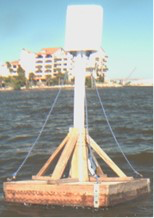
\includegraphics[width=\textwidth]{Images/SDR_bright.png}
        \caption{SDR visual camera (5 MP)}
        \label{fig:SDR_bright}
    \end{subfigure}
    \hspace{2em} % horizontal spacing between them
    \begin{subfigure}[t]{0.378\textwidth}
        \centering
        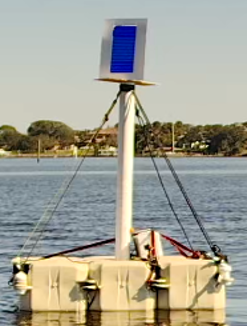
\includegraphics[width=\textwidth]{Images/HDR_bright.png}
        \caption{HDR visual camera (5 MP)}
        \label{fig:HDR_bright}
    \end{subfigure}%
}
\caption{\textcolor{red}{place-holder image – A visual comparison of the \ac{SDR} FLIR 4k camera (left) and the \ac{HDR} Leopard Imaging camera (right) in low-light conditions.}}
\label{fig:HDR_compare}
\end{figure}

In contrast, the Leopard Imaging \ac{HDR} camera offers slightly lower image resolution at a comparable effective focal length but provides substantially greater dynamic range.
% enabling detail preservation across bright and shaded regions within the same frame.  
This wider dynamic range enables more consistent color fidelity and image contrast under suboptimal lighting conditions, as illustrated in Figure~\ref{fig:HDR_compare}.

% Many tasks in the 2024 Maritime RobotX Challenge required \acp{USV} to accurately distinguish object colors as part of their operational decision-making.
This capability motivated the selection of the \ac{HDR} camera as Minion's primary visual camera sensor for the 2024 Maritime RobotX Challenge, which included several tasks that required \acp{USV} to accurately identify object colors in order to make operational decisions.
\textcolor{blue}{Check these results again}\textcolor{blue}{A comparative study by Liebergall et al.~\cite{liebergall} further supported this decision, as preliminary results indicated improved object detection results with data from the \ac{HDR} over the FLIR \ac{SDR} camera.}
Because the data collected during that competition formed the foundation of this dissertation, the Leopard Imaging \ac{HDR} camera, the primary visual spectrum sensor, was selected for all research presented in this paper.

% For these reasons, the \ac{HDR} camera was designated as the primary forward-facing visual spectrum sensor for the \ac{LiDAR}-camera fusion research presented in this paper.  




%%%%%%%%%%%%%%%%%%%%%%%%%%%%%%%%%%%%%%%%%%%%%%%%%%%%%%%%%%%%%%%%%%%%
%%%%%%%%%%%%%%%%%%%%%%%%%%%%%%%%%%%%%%%%%%%%%%%%%%%%%%%%%%%%%%%%%%%%

\subsection{PinPoint GPS/INS} \label{sensors_GPS}

% The Minion platform features a PinPoint \ac{GPS}/\ac{INS} equipped with dual-antennae for orientation and differential corrections for millimeter precision geolocation.
% The sensor performs two critical functions for the \ac{USV}: tracking vessel position and orientation, and precise global time for sensor synchronization.
% The \ac{GPS} receiver functions as the master clock for the entire synchronization hierarchy described in ~\ref{time_sync}, while the integrated \ac{IMU} enables high-rate pose updates between \ac{GPS} fixes.

The Minion \ac{USV} employs a Torc Robotics Pinpoint \ac{GPS}/\ac{INS} unit for both global positioning and inertial navigation capabilities.
This device integrates a differential-corrected \ac{GPS} receiver with a multi-axis \ac{IMU} and dual antenna, providing precise position, velocity, and orientation data for the autonomous platform.
The \ac{GPS} receiver is configured to operate at an update rate of five Hz, while the integrated \ac{IMU} provides high-frequency inertial measurements at 105.4 Hz.
The Pinpoint unit delivers timing accuracy on the order of 10-100 nanoseconds for \ac{GPS}-disciplined time signals, which is a critical function for multi-sensor synchronization discussed in Section~\ref{time_sync}.
% The device interfaces with the vessel's compute infrastructure via Ethernet, configured at IP address 201.7.90.30 on the local network.
% Beyond navigation, the Pinpoint unit serves dual roles: providing a high-accuracy time reference for sensor synchronization and delivering six-degree-of-freedom pose estimates through onboard sensor fusion algorithms.
% The specific methodologies for temporal calibration and synchronization using this device are detailed in Section 3.2.2.1, while the spatial calibration procedures appear in Section 3.2.3.


% Global Navigation Satellite System signals inherently carry highly accurate timing information, as satellite positioning operates through precise measurement of signal delay from multiple satellites with synchronized atomic clocks.
% The PinPoint receiver extracts this timing information and distributes it over the vessel's network using Network Time Protocol.
% The \ac{GPS} unit was assigned a static IP address of 201.7.90.30 on the Minion network and configured to broadcast \ac{GPS}-disciplined time via Network Time Protocol.
% The Atlas PC main computer synchronizes its clock to this \ac{GPS} source with typical accuracy in the tens to hundreds of nanoseconds, limited primarily by network latency rather than \ac{GPS} accuracy.

% This \ac{GPS} time reference propagates through the synchronization hierarchy to every computing resource on the platform.
% Atlas functions as a Network Time Protocol server for the NVIDIA Jetson Xavier camera computer, which subsequently operates as a Precision Time Protocol master for the Livox Horizon \ac{LiDAR} sensors.
% This cascaded approach ensures timestamps from all sensors—cameras, \ac{LiDAR}, and \ac{GPS}/\ac{IMU}—share a common time reference traceable to \ac{GPS} time.

% Beyond timekeeping, the \ac{GPS}/\ac{IMU} system continuously tracks platform position and orientation, which is required for \ac{LiDAR} temporal aggregation.
% As described in Section 3.1.1.3, accumulating \ac{LiDAR} points over several seconds necessitates compensation for vessel motion during that period.
% The PinPoint system fuses \ac{GPS} position measurements with \ac{IMU} acceleration and rotation data through an Extended Kalman Filter to produce pose estimates at rates substantially higher than \ac{GPS} alone could provide.
% \ac{GPS} fixes arrive at 1-10 Hz depending on satellite visibility, while the \ac{IMU} operates at hundreds of hertz.
% The fusion algorithm propagates pose estimates forward using \ac{IMU} integration between \ac{GPS} updates, subsequently correcting accumulated drift when new \ac{GPS} measurements arrive.

% The resulting pose solution provides six-degree-of-freedom state estimates—three-dimensional position and three-dimensional orientation—at sufficient temporal resolution to interpolate platform pose to the exact timestamp of each \ac{LiDAR} point.
% This capability supports the transformation methodology presented in Chapter 5, where \ac{LiDAR} points acquired at different times during motion are transformed to a common reference frame before projection onto camera images.

% The PinPoint \ac{GPS}/\ac{IMU} connects to the Minion computing infrastructure via Ethernet, utilizing both Network Time Protocol for time distribution and User Datagram Protocol for pose data transmission.
% \ac{ROS} driver nodes on the Atlas PC receive and parse the binary \ac{GPS}/\ac{IMU} messages, publishing pose estimates as standard \ac{ROS} geometry messages.
% These messages incorporate position (latitude, longitude, altitude), orientation (roll, pitch, yaw), uncertainty estimates, and \ac{GPS} fix quality flags.
% The \ac{ROS} tf2 library consumes these pose estimates to maintain the time-varying transformation tree relating sensor frames to platform and world frames, enabling automated coordinate transformation for sensor fusion.

% The \ac{GPS}/\ac{IMU} defines the local reference frame for the platform \texttt{base\_link}, with position expressed in geographic coordinates (WGS84 datum) and orientation relative to true north and local gravity.
% This world-referenced system serves as the common reference for transforming observations from multiple sensors acquired at different times during motion.
% Transformation from sensor-local frames to the \ac{GPS}/\ac{IMU} world frame requires knowledge of sensor-to-platform extrinsic calibration parameters.
% These parameters are determined through calibration procedures described in Section 3.2.1.2 for cameras and Section 3.2.1.3 for \ac{LiDAR} sensors.
% With extrinsic parameters established, the \ac{GPS}/\ac{IMU} pose solution enables transformation of any sensor observation to world coordinates or to any other sensor's reference frame.

% Maritime environments present challenges for \ac{GPS}/\ac{IMU} systems that differ from land vehicle applications.
% Water surface reflections induce multipath interference in \ac{GPS} signals, while vessel pitch and roll motion exercises the full range of the \ac{IMU}.
% The PinPoint system was designed for marine applications and incorporates algorithms to address these factors while maintaining accuracy during vessel maneuvering.
% \ac{GPS} accuracy degrades in areas with limited satellite visibility, such as proximity to tall structures, bridges, or fjord-like coastal terrain.
% The \ac{IMU} provides short-term pose continuity during \ac{GPS} outages, though accumulated drift limits the duration for which pure inertial navigation remains accurate.
% Data collection operations were conducted in open water with favorable satellite visibility, ensuring consistent \ac{GPS} fix quality throughout recording sessions.

% The \ac{GPS}/\ac{IMU} system enables two functions essential for multi-modal sensor fusion research.
% First, \ac{GPS}-disciplined time distributed to all sensors ensures timestamps from cameras, \ac{LiDAR}, and \ac{GPS} itself reference the same time base, providing frame-accurate temporal association across modalities.
% Second, continuous pose estimates enable transformation of temporally distributed observations to common reference frames, supporting \ac{LiDAR} aggregation during motion and registration of sensor fields of view for fusion operations.
% Combined with the synchronization verification and drift correction procedures described in Section 3.2.2, these capabilities establish the temporal and spatial foundation for rigorous object detection performance evaluation across sensing modalities.
% The \ac{GPS}/\ac{IMU} thus functions not merely as a navigation sensor but as critical infrastructure enabling the multi-modal perception analysis central to this research.

%%%%%%%%%%%%%%%%%%%%%%%%%%%%%%%%%%%%%%%%%%%%%%%%%%%%%%%%%%%%%%%%%%%%
%%%%%%%%%%%%%%%%%%%%%%%%%%%%%%%%%%%%%%%%%%%%%%%%%%%%%%%%%%%%%%%%%%%%
\section{Compute Hardware and Network} \label{sec:Atlas_LAN}

Minion distributes processing tasks across multiple computing nodes to achieve real-time performance and robust system operation.
The computing infrastructure consists an embedded computer integrated with the camera sensors for video encoding and streaming, and twin computers serving as the primary processing platforms, with a \ac{GbE} \ac{LAN} connecting all systems and sensors. 
% This architecture distributes computational workloads according to sensor proximity and processing requirements while maintaining centralized coordination through the Robot Operating System middleware. 
The following subsections detail the hardware specifications, system architecture, and network infrastructure that enable real-time multi-modal perception for maritime object detection and sensor fusion.

%%%%%%%%%%%%%%%%%%%%%%%%%%%%%%%%%%%%%%%%%%%%%%%%%%%%%%%%%%%%%%%%%%%%
\subsection{Camera Enclosure} \label{comp:camera_enclosure}

% # Camera Enclosure Computing Platform

% for the RobotX competition in 2022, as well as the PhD research of D. Thompson \cite{thompson2023}.
% Specialized computing hardware is required to manage up to six video streams from the cameras within the enclosure.
% The camera enclosure assembly integrates six camera sensors with dedicated computing hardware housed in a weatherproof enclosure mounted on the vessel's superstructure. 


% real-time H.264/H.265 video encoding, manages timestamp embedding for temporal synchronization, and serves critical time distribution functions within the hierarchical clock architecture. This distributed computing approach places video processing at the camera location rather than transmitting raw uncompressed video over the network, substantially reducing bandwidth requirements while enabling sophisticated in-stream timestamp embedding.

% The camera enclosure houses six cameras and serves as the mount for the three forward Livox LiDAR units, and was designed to be a self-contained perception platform for any maritime vessel or ground vehicle. 
The camera enclosure serves as the integrated perception module for the vessel, and was designed as a self-contained sensor and computing subsystem that can operate independently on any maritime or ground vehicle. 
Integrated into this subsystem is a NVIDIA Jetson AGX Xavier, a compact and capable PC designed for video processing, as well as other computer vision applications.
% The system-on-module (SOM) design combines ARM-based CPU cores with a powerful GPU architecture optimized for media encoding and AI tasks. 
% The system-on-module (SOM) design integrates a processor, GPU, and memory in a compact form factor designed for speed and power efficiency.
Key hardware specifications are provided in table \ref{table:Xavier_hardware}.
% The Jetson AGX Xavier serves as the dedicated processing unit within the camera enclosure, managing video acquisition, compression, and transmission from all six cameras.  

Its 8-core ARM processor provides ample computational capacity for handling multiple video pipelines, network protocols, and system-level services, while the integrated 512-core Volta GPU performs hardware-accelerated video encoding required for concurrent high-resolution streams.  
A unified memory architecture shares 32 GB between the CPU and GPU and supports a memory bandwidth of 136.5 GBps, which minimizes latency and improves overall pipeline efficiency.

Each video feed follows a two-branch processing pipeline.  
% Raw frames are captured over USB~3.0 and parsed by custom software before being distributed to parallel encoding tasks. 
Raw video frames are received via USB 3.0, parsed by custom software, and then split into two processing branches. 
One branch is encoded in H.265 and saved locally to the Jetson's internal storage, while the other branch is down-sampled to a reduced frame rate before being streamed over the \ac{LAN} to one of the Minion PCs in Atlas.



% ## NVIDIA Jetson Xavier Platform
% The Jetson Xavier’s 8-core ARM processor provides ample computational capacity for managing multiple video pipelines, network protocols, and system services, while the integrated 512-core Volta GPU enables hardware-accelerated video encoding required for concurrent high-resolution stream processing.  
% A shared 32~GB pool of unified memory between the CPU and GPU supports high-throughput data exchange, ensuring efficient media handling and minimizing latency within the video processing pipeline.

% % \subsubsection{Video Processing Architecture}
% The primary computational responsibility of the Jetson Xavier is video encoding and transmission of video from the six cameras.
% % three 4K cameras, two FLIR, and a single HDR camera feeds. 
% The pipeline for each video follows a similar structure: raw video frames are received via USB 3.0, parsed by custom software, and then split into two processing branches. 
% One branch is encoded in H.265 and saved locally to the Jetson's internal storage, while the other branch is down-sampled to a reduced frame rate before being streamed over the \ac{LAN} to one of the Minion PCs in Atlas.

\begin{table}[htpb]
\centering
\begin{tabular}{ll}
\hline
\multicolumn{2}{c}{NVIDIA Jetson AGX Xavier} \\
\hline
% \textbf{Component} & \textbf{Specification} \\
\hline
Processor (CPU) & 64-bit 8-core NVIDIA Carmel \\
Graphics (Integrated) & 512-core NVIDIA Volta \\
Memory (RAM) & 32 GB LPDDR4 \\
Memory Bandwidth & 135 GBps \\
Storage (Primary) & 32 GB eMMC 5.1 \\
Storage (Secondary) & 500 GB NVMe \\
Network Interface & Gigabit Ethernet \\
Operating System & Ubuntu 18.04 \\
\hline
\end{tabular}
\caption{NVIDIA Jetson Xavier - Hardware and Operating System Specifications}
\label{table:Xavier_hardware}
\end{table}

This reduction in frame rate is essential to maintain reliable network performance given limited bandwidth, as discussed in Section \ref{comp:network}. 
The maximum bitrate $R_{\text{max}}$ of each stream is computed at runtime as a function of the target frame rate, frame resolution, and compression ratio, defined by

\begin{equation}
    R_{\text{max}} = N_x N_y b f
\end{equation}

where $N_x$ and $N_y$ are the image width and height in pixels, $f$ is the desired frame rate, and $b$ is the effective bits per pixel after compression.
For the HDR camera, the image resolution is $2880 \times 1860$ pixels, encoded in YUV 4:2:0 format using H.264 compression.
An empirically derived constant of $b = 0.14$ bits per pixel captures the combined effects of color subsampling and compression efficiency under typical scene conditions.
These values yield a bitrate for the HDR camera of
\begin{equation*}
    \begin{split}
        R_{\text{max}} & = (2880 \times 1860\; \text{px}) (0.14 \;\text{bits/px})(5\;\text{s}^{-1})  \\
        & \approx 3.75\; \text{Mbps}
    \end{split}
\end{equation*}

and scales linearly with frame rate.
This adaptive bitrate approach ensures that each video stream remains within the available network bandwidth while maintaining adequate visual fidelity for perception and data logging.
By default, each camera operates at 5 \ac{fps}, aligning with the data rate of other perception sensors, but this rate can be adjusted as needed. % to accommodate specific mission or testing requirements.


% Each camera stream defaults to 5 \ac{fps} to match the data rate of other perception data, but can be modified based upon need.
% This  us a default maintaining each stream below 25–30 Mbps to prevent network saturation.
% This ensures bandwidth allocation per stream remains within network limits while preserving visual fidelity.

While compressed video is streamed to Atlas, the Jetson simultaneously records each feed at its native frame rate to the onboard 500 GB solid-state NVMe drive as redundant backups. 
Each recording is saved in 120-second segments along with a corresponding \ac{CSV} file pairing every image frame with a timestamp from the system clock. 
The same system clock provides the \ac{PTP} signal used by the Livox LiDAR units. ensuring consistent temporal alignment across all sensors within the perception suite. 
Consequently, the timestamps in the recorded \ac{CSV} files are also essential for validating the synchronization of the camera and LiDAR, as discussed in Section \ref{time_sync_cam}.

% Local recording also serves diagnostic purposes, enabling comparison of locally-saved video files with network-transmitted ROS bag data to validate timestamp accuracy and detect any frame dropping or duplication during network transmission. The temporal drift analysis methodology described in Section \ref{time_sync_cam} exploits this local recording capability by comparing locally-saved video frames with network-transmitted ROS messages to quantify systematic timing offsets introduced by the encoding-transmission-decoding pipeline.


% The video encoding workflow exploits the Jetson's dedicated hardware encoding engines to achieve real-time compression of three simultaneous 2880×1860 pixel video streams. Hardware encoding offloads the computationally intensive compression operations from the CPU, enabling sustainable operation without thermal throttling during extended recording sessions. The RTSP bitrate is [INSERT bitrate formula here] dependent upon the requested stream frame rate (typically 5-15 fps).

% The compressed video streams are transmitted to the Atlas PC main computing platform via RTSP over UDP, where they are decoded and published as ROS image messages for consumption by object detection algorithms. This architecture distributes the encoding burden to the camera enclosure while centralizing detection processing on the more powerful Atlas hardware.

% A critical function performed by the Jetson Xavier is the embedding of precise system timestamps directly into the encoded video bitstream. Custom GStreamer pipeline elements inject SEI (Supplemental Enhancement Information) NAL units containing synchronized timestamps alongside encoded video frames. This in-band metadata approach ensures that timing information persists with the video data through network transmission, recording, and playback. The temporal synchronization procedures and timestamp validation methodology are detailed in Section \ref{time_sync_cam}.

% \subsubsection{Network Infrastructure Role}

% Within Minion's distributed computing architecture, the Jetson Xavier subscribes to the precise GPS clock provided by the Pinpoint.

% erves several network infrastructure functions. As described in Section \ref{time_sync_lan}, the system participates 

% in the hierarchical time distribution network that provides temporal synchronization for all platform sensors. The Jetson operates as both a client for receiving GPS-disciplined time and a server for providing high-precision timing to the LiDAR sensors.

% The Gigabit Ethernet interface connects the camera enclosure to the vessel local area network at IP address 201.7.90.147. This single network connection carries bidirectional traffic including compressed video streams, time synchronization protocols, remote administration access, and platform status monitoring. The camera enclosure may also include a secondary Ethernet switch to provide local network connectivity for the three Livox Horizon LiDAR units mounted on or near the camera mast, as detailed in Section \ref{comp:camera_enclosure}.

% \subsubsection{Local Recording Capability}


%%%%%%%%%%%%%%%%%%%%%%%%%%%%%%%%%%%%%%%%%%%%%%%%%%%%%%%%%%%%%%%%%%%%
\subsection{Atlas} \label{atlas}

The primary computing infrastructure consists of two identical high-performance workstation computers, designated Minion A and Minion B.  
Built with enterprise-grade components, these systems provide the computational resources required for real-time sensor processing, object detection, and autonomous navigation.
Table~\ref{table:Minion_hardware} summarizes the key system specifications.
The dual-computer configuration enables parallel software development and operational redundancy, with one system dedicated to production tasks while the other supports software testing or serves as a backup.
 
Minion A was configured with Ubuntu 22.04 for the development and migration of Minion's software to ROS 2 Humble, while 
Minion B served as the only device used for data-recording and object-detection processing performed for the research of this dissertation, and ran Ubuntu 20.04 with ROS 1 Noetic.

% While ROS manages sensor data and transforms between reference frames, the focus in this section relates to the underlying hardware responsible for real-time, multi-modal perception.  
% The object-detection methods described in Chapter \ref{realtime_object_detection} are optimized for the computational characteristics of the CPU and GPU.  
% This distribution of processing responsibilities balances throughput, latency, and efficiency across the perception pipeline.  
% The following subsections describe how LiDAR and vision workloads are allocated between the CPU and GPU on the Atlas platform.

% While the ROS middleware manages communication and synchronization between sensor nodes, the emphasis here is on the computational workload executed by the Atlas hardware. 

% Perception processing is divided between CPU and GPU resources according to the characteristics of each object detection method.  
% LiDAR-based object detection, is performed on the CPU due to its reliance on irregular memory access patterns and control flow.  
% Conversely, vision-based detection utilizes parallel tensor operations that the GPU hardware is optimized for.  
% This allocation of workloads balances computational throughput and latency, ensuring reliable multi-modal perception and sensor fusion for autonomous operation.

% primarily between the CPU and GPU according to algorithm characteristics and hardware acceleration capabilities.

% have different workload requirements, and therefore operate primarily on separate processing units.
% Perception workloads are 
% This 
% While \ac{ROS} manages coordination and communication across processes, the following overview focuses on the hardware-level execution of LiDAR and vision tasks.

% \subsubsection{CPU and Memory}
% Each Atlas PC is equipped with computing hardware selected to meet the demanding real-time requirements of multimodal perception and autonomous operation.  
% % Table~\ref{table:Minion_hardware} summarizes the key system specifications.
% The Intel Xeon processor provides six cores and a total of twelve parallel threads for concurrent perception and navigation processes.
% Tasks that require low-latency responses—such as LiDAR point cloud filtering and sensor updates benefit from the processor’s strong single-thread performance.
% % , which minimizes delay between sensor input and system response.  
% At the same time, the multi-core architecture supports parallel execution of computationally intensive workloads.
% % , including feature extraction and classification across multiple LiDAR streams.  
% Hardware vector acceleration further enhances numerical operations common to point cloud transformations and coordinate frame calculations.

% The system’s 16~GB of high-bandwidth memory provides sufficient capacity to buffer LiDAR point clouds, video imagery, and other sensor data during real-time processing.  
% This configuration allows multiple perception modules to access and update shared data concurrently without slowing overall system performance.

% \subsubsection{CPU and Memory}
Each Atlas PC is equipped with computing hardware selected to meet the real-time requirements of multimodal perception and autonomous operation.  
The Intel Xeon processor features six cores and twelve parallel threads that support concurrent execution of perception and navigation processes.  
Tasks requiring low-latency response, such as LiDAR point-cloud filtering and sensor updates, benefit from the processor’s strong single-thread performance, while the multi-core architecture efficiently handles computationally intensive workloads.  
Hardware vector acceleration further enhances numerical operations common to point-cloud transformations and coordinate-frame calculations.

The system’s 16 GB of high-bandwidth DDR4 memory provides sufficient capacity to buffer LiDAR point clouds, video imagery, and navigation data, while offering the throughput necessary for their continuous exchange between processing threads.  
This configuration ensures that shared data structures remain accessible without introducing latency, maintaining consistent performance during extended autonomous operation. 
% This configuration ensures that shared data structures remain accessible across multiple processing threads without introducing latency, maintaining consistent timing performance during extended autonomous operation.

\begin{table}[htpb]
\centering
\begin{tabular}{ll}
\hline
\multicolumn{2}{c}{Minion PC - Hardware Specification} \\
\hline
\hline
Processor (CPU) & Intel Xeon E5-1650 v3 \\
CPU Cores & 6-core / 12-thread, 3.50 GHz \\
Graphics (GPU) & NVIDIA GeForce GTX 1080 \\
GPU Memory & 8 GB GDDR5X, 2560 CUDA cores \\
Memory (RAM) & (4x) 4 GB DDR4 \\
Storage (Primary) & 500 GB NVMe SSD \\
Network Interface & (6x) Gigabit Ethernet \\% + 802.11ac WiFi \\
\hline
\end{tabular}
\caption{Minion A/B PC Hardware Specifications}
\label{table:Minion_hardware}
\end{table}

% \subsubsection{GPU}

% The NVIDIA GTX~1080 GPU accelerates the vision-based object detection pipeline by handling tasks that benefit from highly parallel computation.  
% Its primary responsibilities include decoding the incoming video streams from the camera enclosure and performing the image convolution operations required for vision-based detection.  
% The GPUs have hardware-accelerated video encoders and decoders for processing multiple video streams, and an object-detection algorithm was written to leverage the 2,560 CUDA cores for fast tensor and matrix computations and image convolution.
% This also offloads H.264 decompression from the CPU, allowing the system to process multiple high-resolution camera streams simultaneously while preserving CPU resources for LiDAR and sensor-fusion tasks.

  
% These operations are executed directly in GPU memory, leveraging  cores  the repetitive tensor and matrix computations common to neural network inference.  
% This hardware acceleration enables real-time image processing and object detection performance that would otherwise be infeasible on CPU resources alone.

% Each GTX 1080 GPU features 2560 CUDA cores based on NVIDIA's Pascal architecture with 8 GB of GDDR5X memory, accelerating both machine learning inference for object detection video decoding tasks.
% The Pascal architecture provides CUDA compute capability 6.1, enabling efficient execution of YOLOv8 convolutional neural networks and GPU-accelerated image preprocessing described in Chapter \ref{realtime_object_detection}.
% Hardware video decode engines offload H.264 video decompression from the CPU, enabling the Atlas PC to receive and process multiple camera streams simultaneously while maintaining CPU resources for perception algorithms.

% \subsubsection{GPU}

The GPU is Atlas's primary processor for the system’s vision pipeline, handling both video decoding and neural network inference for object detection.
Each GTX~1080 features 2,560 CUDA cores built on NVIDIA’s Pascal architecture with 8~GB of GDDR5X memory, providing the computational throughput required for highly parallel image-based workloads.  
  
Incoming video streams from the camera enclosure are first decoded using hardware-accelerated video codecs, enabling efficient processing of multiple high-resolution feeds.
The resulting frames are again passed to the GPU for accelerated tensor calculations and neural network based algorithms described in Chapter \ref{realtime_object_detection} for object detection.
% NVIDIA's CUDA architecture has long been the industry standard for efficient execution of convolutional neural networks such as YOLOv8.

Executing both video decoding and inference workloads on the GPU frees up valuable system resources for LiDAR processing and sensor fusion tasks.

% \subsubsection{Workload Allocation}

% The CPU-GPU task distribution reflects algorithm characteristics and hardware capabilities.
% LiDAR processing with irregular spatial queries and dynamic data structures exploits CPU cache hierarchies and branch prediction, while vision processing with regular tensor operations and data parallelism leverages GPU throughput.
% The 6-core CPU handles approximately 3× simultaneous LiDAR processing streams plus sensor fusion logic without saturating computational resources, while the 2560-core GPU processes vision workloads that would overwhelm CPU execution.

% This balanced allocation maintains real-time performance with sub-100 millisecond end-to-end latency from sensor observation to fused detection output, meeting the temporal requirements for autonomous navigation decision-making.
% Load monitoring during typical operations indicates approximately 60-70\% CPU utilization across all cores and 70-80\% GPU utilization during simultaneous LiDAR and vision processing, providing margin for computational bursts during high-complexity scenes.

% % \paragraph{CPU-Based Processing}

% LiDAR point cloud processing and LiDAR-based object detection are executed on the system’s multi-core CPU.
% These algorithms involve spatial clustering, coordinate transformations, and probabilistic data association—operations that rely on irregular memory access patterns and branching logic.
% Such workloads benefit from the CPU’s high single-threaded performance, cache hierarchy, and flexible memory management.
% The CPU also performs sensor fusion between LiDAR and vision detections, as well as general system coordination tasks such as recording data. %, network management, and operator interface control.

% % \paragraph{GPU-Based Processing}

% The GPU accelerates two perception tasks that exhibit a high degree of data parallelism: video decoding and deep learning inference.
% Its first responsibility is processing video streams received from the camera enclosure. 
% Video decoding and image preprocessing are performed directly in GPU memory, minimizing data transfer overhead and reducing end-to-end latency.
% The second responsibility is image-based object detection using the \ac{YOLO} framework. 
% This algorithm relies on convolutional and tensor operations within neural networks and is implemented to leverage the parallel processing capabilities of NVIDIA’s CUDA architecture.

% \subsubsection{Storage Media}

High-speed solid-state storage provides the throughput required to record multiple sensor streams during data collection operations.
Each recording session captures raw \ac{LiDAR} point cloud data, uncompressed video imagery, GPS/INS pose information, and mapped object-detection results, producing aggregate data rates that can easily exceed 200 \ac{MBps}.
A solid-state NVMe hard drive is used on each Minion system to provide the data throughput that these operations require, and is much more robust to the motion experienced in choppy surf and vibrations experienced while in transport on the \ac{USV}'s trailer.
% and 5–15MBps per camera for H.265-compressed video at 10~fps, with additional low-bandwidth streams for GPS/INS and detection results.
% The NVMe solid-state drives provide sufficient sequential throughput and IOPS to maintain these rates for extended sessions without frame loss or buffer overflow.

% \textcolor{red}{If time allows, it may be worth mentioning the cooling system.}



%%%%%%%%%%%%%%%%%%%%%%%%%%%%%%%%%%%%%%%%%%%%%%%%%%%%%%%%%%%%%%%%%%%%
\subsection{Network Structure} \label{comp:network}

Each device on the network is assigned a static IP address on the network, allowing deterministic communication between endpoints.
Camera streams from the Jetson Xavier, point cloud data from each LiDAR sensor, and other telemetry are transmitted over the LAN to Atlas, where sensor data are processed locally.
Data of mapped and detected objects and other system commands, such as motor control commands, are published along with the raw data as \ac{ROS} message topics for system monitoring and data recording.

Under normal operation, the combined network traffic only utilizes about 15\% of the Gigabit Ethernet capacity, 
leaving sufficient headroom for motor control, system services, and remote access for administrative functions.
However, when \ac{ROS} data topics are broadcast across the network for visualization or debugging, bandwidth utilization can temporarily spike and saturate the network.
For this reason, ROS data is recorded locally, and admin visualization tools such as RVIZ are typically restricted to smaller topics related to object mapping and system controls.
A high-level overview of network utilization is provided in Table \ref{table:network_bandwidth}.

\begin{figure}[htbp]
\centering
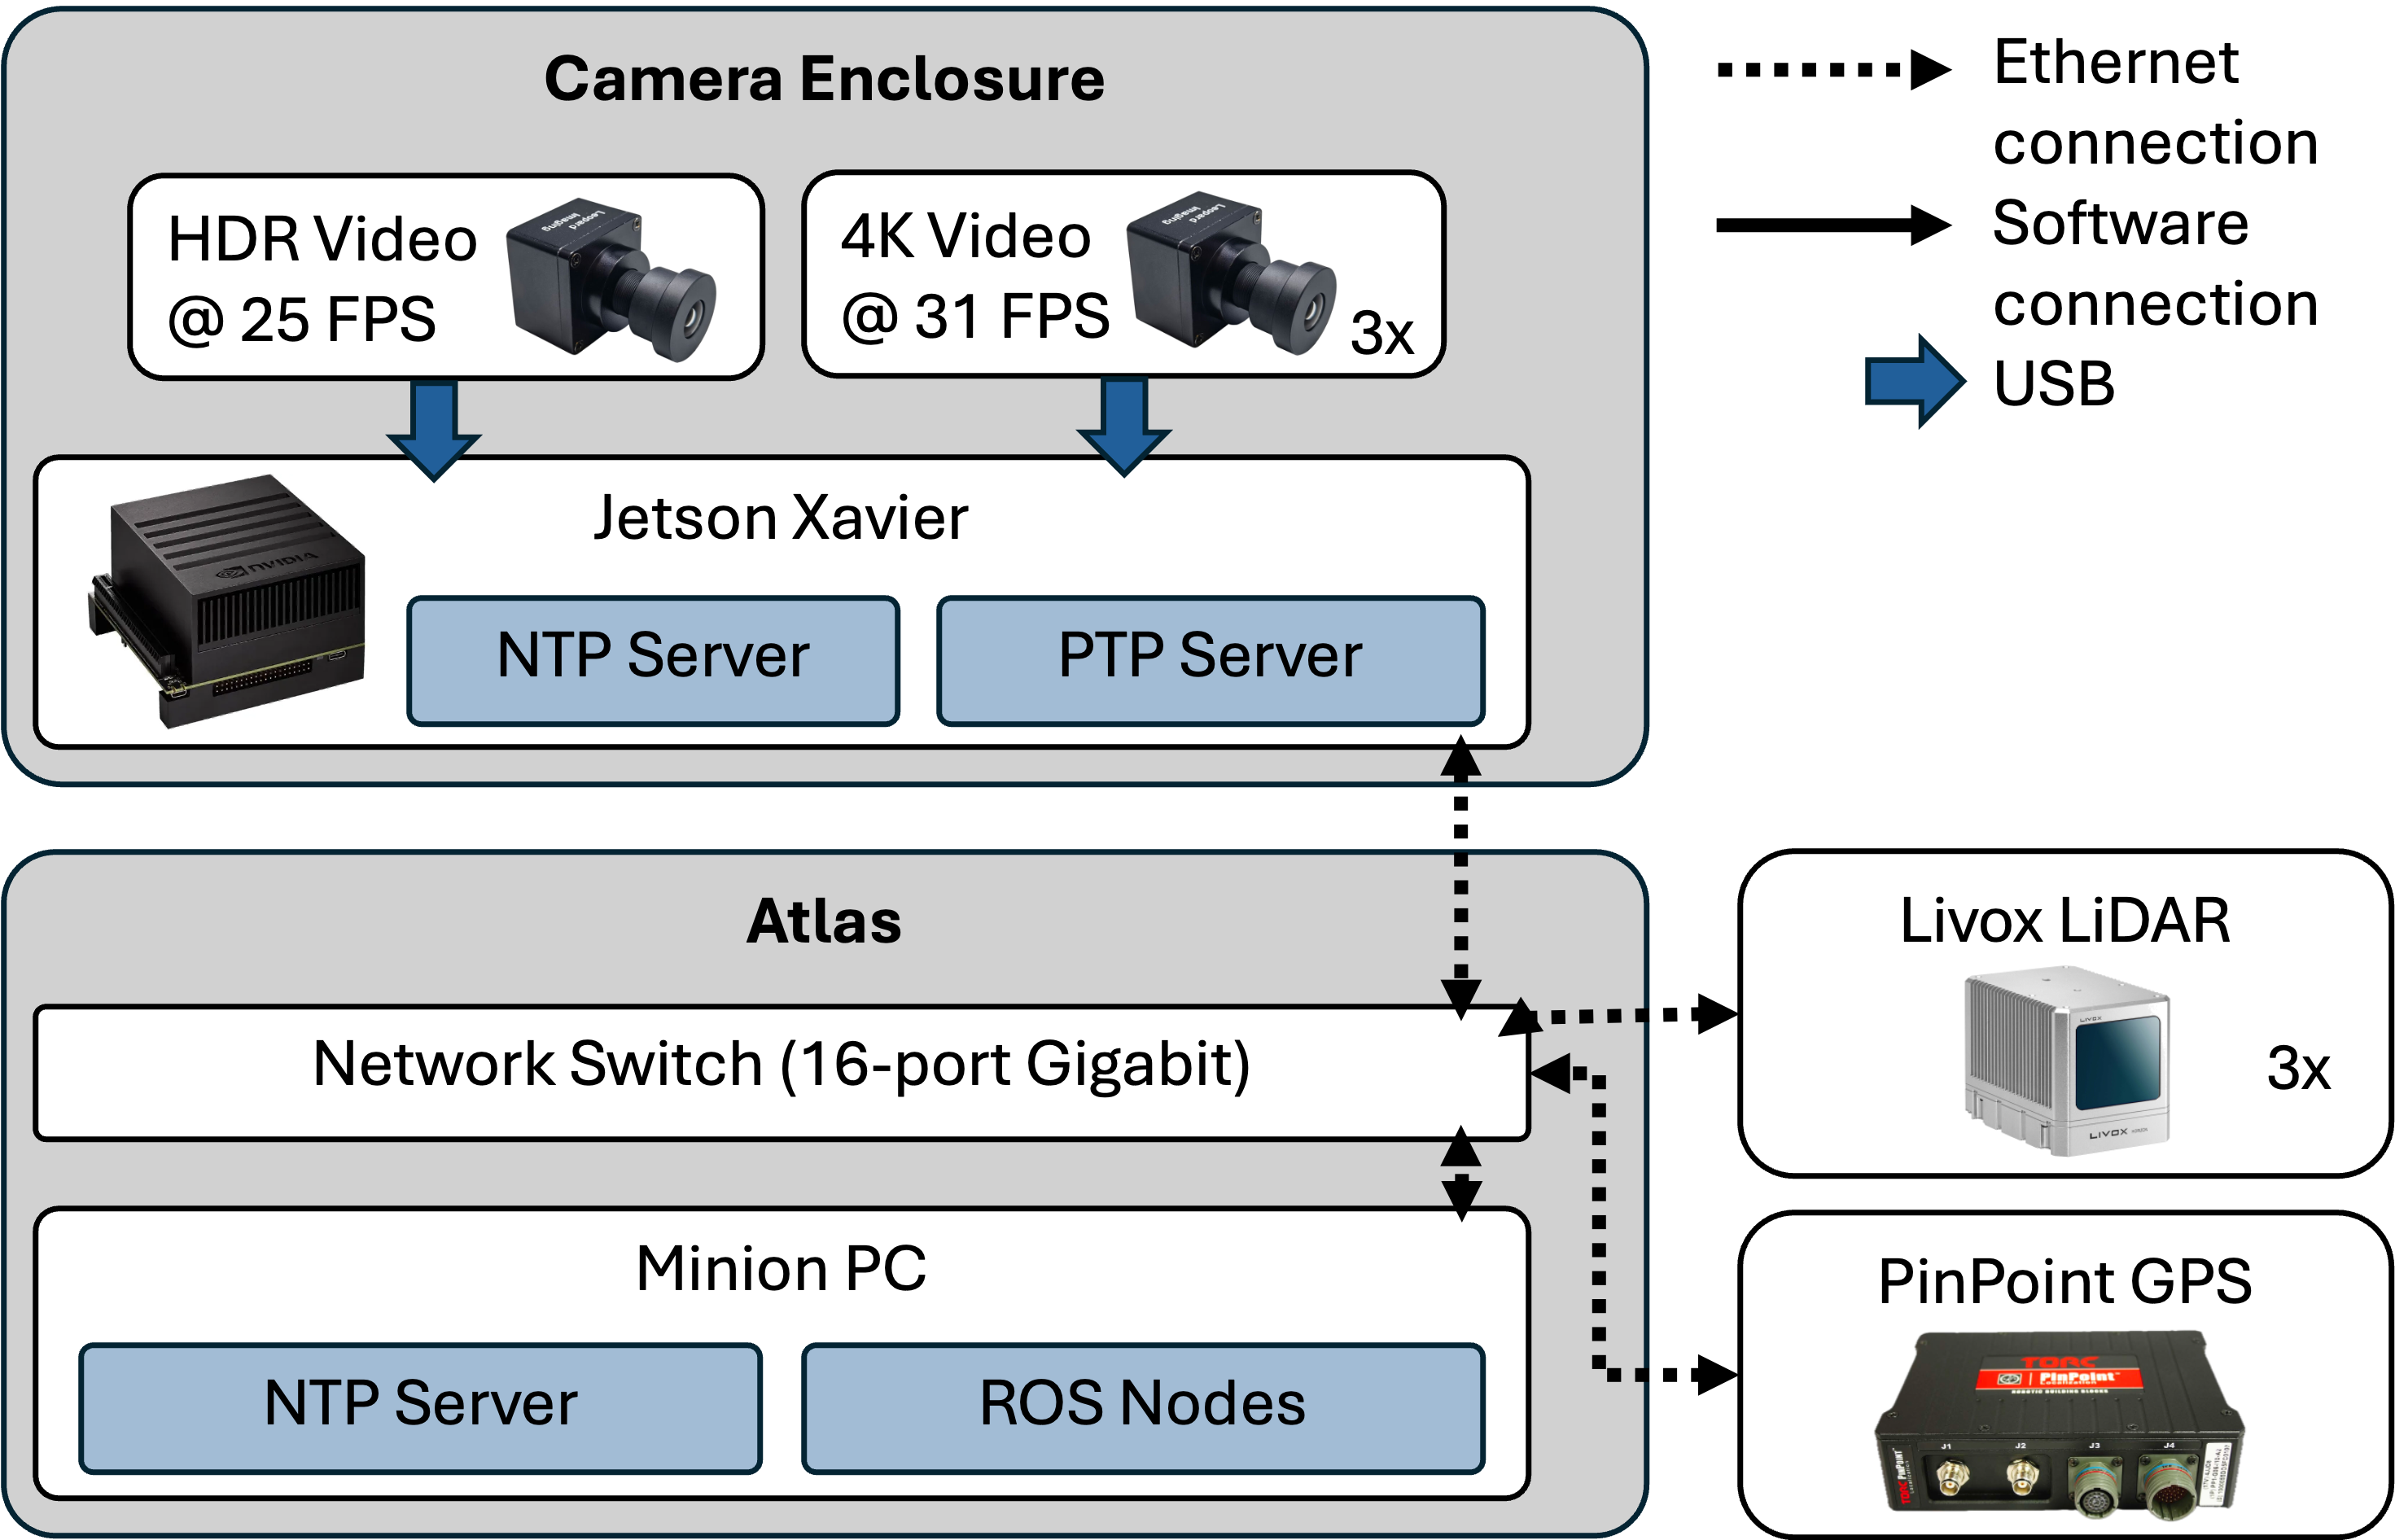
\includegraphics[width=0.8\textwidth]{Images/network_diagram2.png}
\caption{LAN diagram for Minion USV}
\label{fig:network_diagram}
\end{figure}

Although the LAN is primarily dedicated to perception and data logging, it also supports administrative access for configuration, diagnostics, and remote operation.
The Jetson Xavier is configured as a headless device and is accessed remotely via Secure Shell (SSH) for camera configuration, operation, and monitoring.
Each Minion PC can be accessed through SSH for terminal access for development tasks or troubleshooting, or Virtual Network Computing (VNC), and Remote Desktop Protocol (RDP) for a full desktop environment for system administration.
% Network security is intentionally lightweight for field deployment, relying on standard \texttt{sudo}/root authentication and a secured wireless link protected by a strong \ac{WAN} password.
Long-range connectivity between the vessel and ground station is provided by a Ubiquiti Bullet omnidirectional antenna on the \ac{USV}, paired with a directional antenna and a Ubiquiti Dream Machine at the ground station for remote system access and monitoring.

\begin{table}[htbp]
\centering
\begin{tabular}{lcc}
\hline
Data Source & Typical Bandwidth (Mbps) & \% Total Bandwidth \\
\hline
HDR Camera Stream & $3.7$--$11.2$ & $0.4$--$1.2$ \\
FLIR Camera Streams (2×) & $7.0$--$20.0$ & $0.7$--$2.1$ \\
Velodyne LiDAR Units (3x) & $43.2$--$57.6$ & $4.3$--$5.8$ \\
Livox LiDAR Units (3x) & $40.3$--$53.8$ & $4.0$--$5.4$ \\
GPS / INS Telemetry & $<0.1$ & $<0.01$ \\
Admin / SSH / Control Traffic & $0.5$--$2.0$ & $0.05$--$0.2$ \\
\hline
\textbf{Total Estimated Utilization} & \textbf{95--145 Mbps} & \textbf{9.5--14.5 \%} \\
\hline
\end{tabular}
\caption{Approximate network bandwidth utilization from direct sensor and control data sources relative to a 1 Gbps link ($\sim940$ Mbps usable).}
\label{table:network_bandwidth}
\end{table}



% The Minion autonomous surface vessel employs a dedicated Gigabit Ethernet local area network to interconnect computing platforms, sensors, and navigation equipment. 
% This network serves multiple critical functions: sensor data transmission, \ac{NTP} for system clock synchronization, and remote administration access for communication to the \ac{ROS} middleware. 
% Figure \ref{fig:network_diagram} presents a block diagram of the connected network endpoints required for sensor fusion.

% All computing platforms and sensors maintain fixed addresses throughout system operation, enabling deterministic routing and simplified network administration.




% The local network architecture connects all major perception and processing nodes within the vessel and provides a unified temporal reference across systems.
% Time synchronization is managed hierarchically through GPS, Chrony, and PTP, ensuring consistent timestamps for all recorded data streams.

% At the top of the synchronization hierarchy, the Pinpoint GPS/INS unit provides a GPS-disciplined Network Time Protocol (NTP) reference to both the Atlas PC and the Jetson Xavier via the onboard router. Each device runs the Chrony service (Ubuntu 18.04), which continuously aligns the local system clock to the GPS reference with sub-millisecond accuracy.

% \begin{figure}[htbp]
% \centering
% 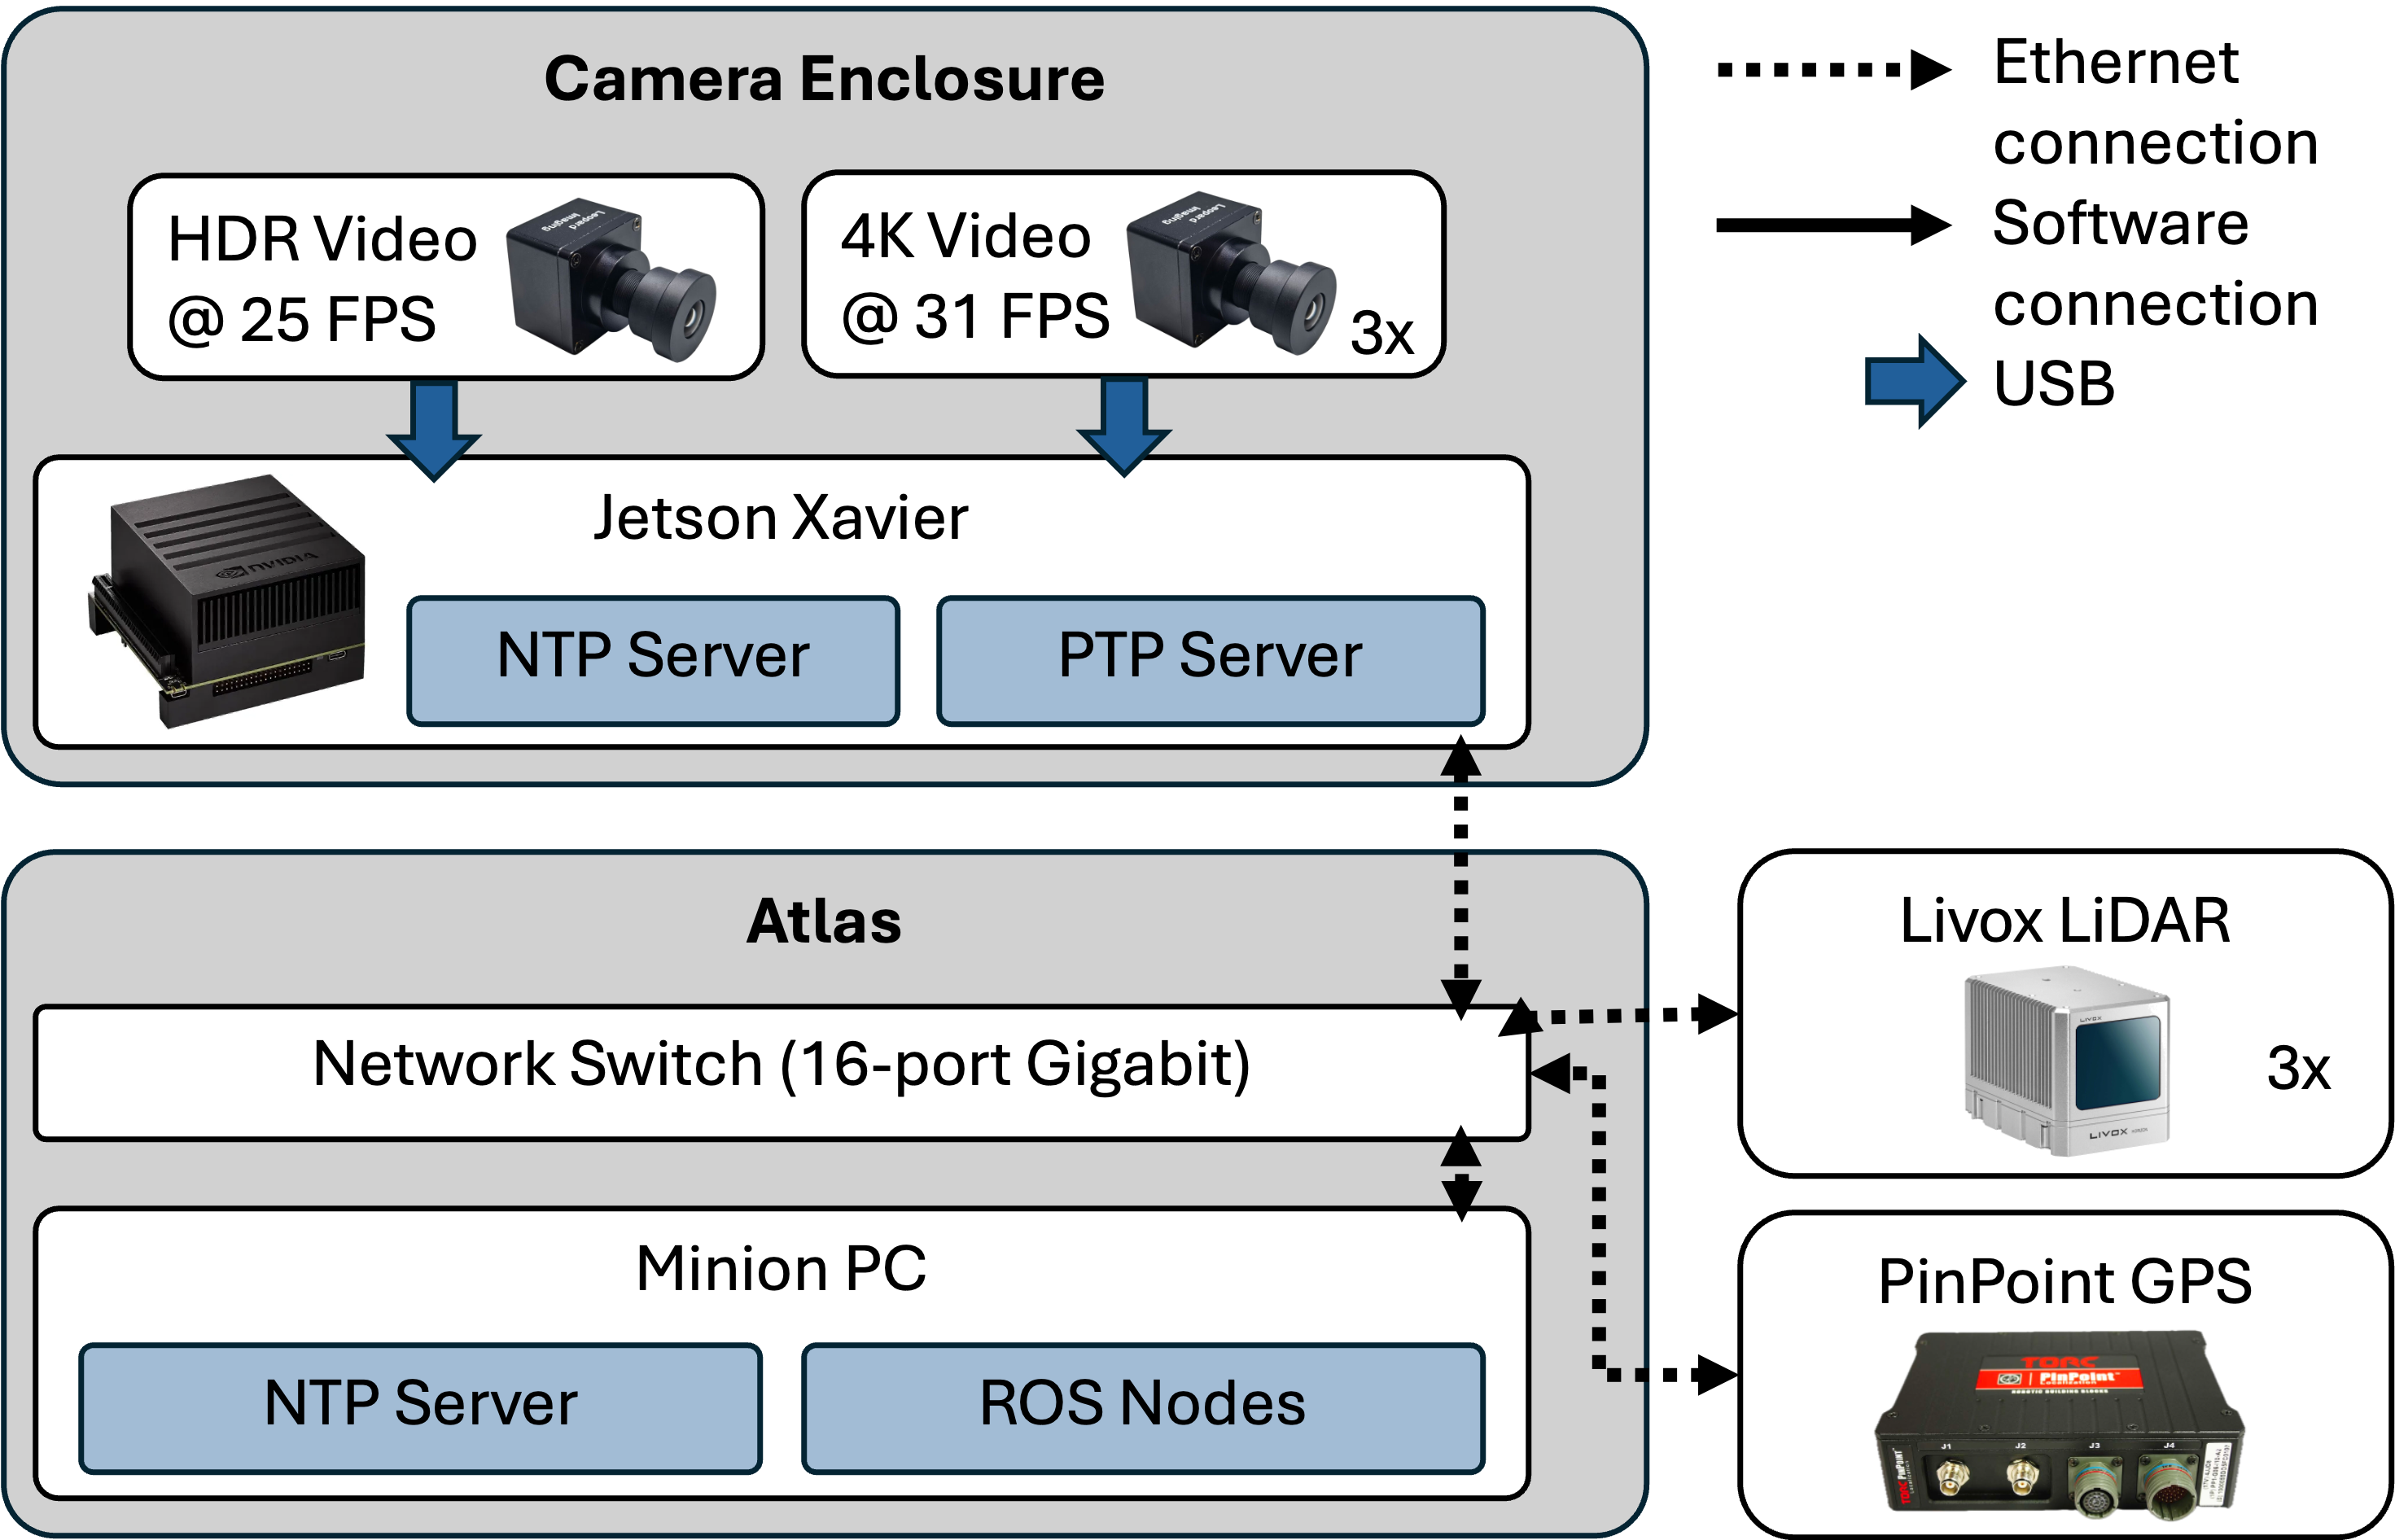
\includegraphics[width=0.8\textwidth]{Images/network_diagram2.png}
% \caption{Minion's LAN for network end-points related to real-time object detection}
% \label{fig:network_sync}
% \end{figure}

% The Jetson Xavier, serving as the core perception node, then acts as the PTP master for the Livox LiDAR units. Through the Precision Time Protocol (IEEE 1588), the Jetson broadcasts high-precision timestamps to all connected LiDAR clients, achieving microsecond-level synchronization between video and LiDAR data streams. This configuration ensures that every sensor measurement—image frame, LiDAR scan, or GPS fix—is temporally aligned to a common reference frame, enabling accurate data fusion and calibration as described in Section \ref{time_sync_cam}.

% Network bandwidth allocation is carefully managed to prevent congestion during real-time operation.
% Each Jetson video stream dynamically adjusts its bitrate based on the active frame rate, while LiDAR and telemetry traffic maintain constant low-latency channels.
% Table \ref{table:network_bandwidth} summarizes the approximate bandwidth usage across major network components.

% \begin{table}[htbp]
% \centering
% \begin{tabular}{lcc}
% \hline
% \textbf{Data Source} & \textbf{Protocol / Port} & \textbf{Typical Bandwidth (Mbps)} \\
% \hline
% HDR Camera Stream (Jetson $\rightarrow$ Atlas) & RTP / UDP & 3.7–11.2 \\
% FLIR Camera Streams (2x) & RTP / UDP & 7.0–20.0 (total) \\
% Livox LiDAR Units (3x) & UDP / PTP Client & 15.0–18.0 (total) \\
% GPS / INS Telemetry & NMEA / TCP & $< 0.1$ \\
% PTP Synchronization Packets & IEEE 1588 / UDP & $< 0.01 $\\
% \hline
% \textbf{Total Estimated Utilization} & — & \textbf{25–50 Mbp/s} \\
% \hline
% \end{tabular}
% \caption{Approximate Network Bandwidth Utilization}
% \label{table:network_bandwidth}
% \end{table}

% Security considerations for remote access include firewall configuration to restrict inbound connections, authentication requirements for SSH administrative access, and potential disconnection of external network access during sensitive operations to prevent unauthorized interference. The remote access infrastructure facilitates collaboration between multiple researchers working on different system components, as well as monitoring by shore-based personnel during extended autonomous operations.

% \subsubsection{Integration with Distributed Computing Architecture}

% The network infrastructure provides the physical medium for the distributed computing architecture that spans multiple platforms. The Jetson Xavier camera enclosure performs video encoding at the sensor location, transmitting compressed streams to the Atlas PC for object detection processing. This distribution optimizes bandwidth utilization by avoiding transmission of raw uncompressed video while maintaining centralized processing for computationally intensive algorithms.



% \subsubsection{Network Performance Validation}

% Network performance validation procedures employed during system commissioning verify that the infrastructure meets requirements for real-time perception and control. These procedures include bandwidth testing using iperf3 or similar tools to verify Gigabit link speeds between key endpoints, latency measurement via ping utilities to measure round-trip latency for time-critical paths, packet loss assessment through extended ping tests or UDP stream analysis to verify zero packet loss under load, and time synchronization quality monitoring to confirm clock accuracy meets requirements as detailed in Section \ref{time_sync_lan}.

% These validation procedures ensure that the network infrastructure meets the performance requirements necessary for real-time multi-modal perception and accurate temporal alignment of sensor data. Baseline performance metrics established during commissioning provide reference values for ongoing network health monitoring during field operations.

%%%%%%%%%%%%%%%%%%%%%%%%%%%%%%%%%%%%%%%%%%%%%%%%%%%%%%%%%%%%%%%%%%%%
%%%%%%%%%%%%%%%%%%%%%%%%%%%%%%%%%%%%%%%%%%%%%%%%%%%%%%%%%%%%%%%%%%%%
% \section{Sensor Calibration} \label{sec:calibration}

% The multi-sensor perception suite described in the previous section integrates complementary sensing modalities: \ac{LiDAR} for spatial structure and cameras for visual context.
% Each of these sensors measures the environment within its own reference frame and according to its own internal clock.
% To combine their observations into a consistent world model, the system must first be calibrated both spatially and temporally.

% Spatial calibration establishes the geometric relationships among all sensing elements.
% It quantifies each sensor’s intrinsic parameters—those governing the internal projection or ranging model—and the extrinsic transformations that define their relative positions and orientations within the overall platform.
% In the context of this work, the global chain of spatial relationships is implemented in the \ac{ROS} \texttt{tf\_tree}, linking coordinate frames from the \ac{GPS} and inertial reference through each \ac{LiDAR} unit to the visible-spectrum cameras.
% Accurate spatial calibration ensures that a point detected in a \ac{LiDAR} scan can be correctly projected onto the image plane, enabling correspondence between geometric and visual detections for downstream fusion.

% Temporal calibration aligns sensor data streams in time, ensuring that observations correspond to the same physical instant.
% Because each device maintains its own internal clock and sampling rate—\ac{LiDAR} operating at 100Hz with microsecond timestamps and cameras capturing 10Hz video with millisecond precision—even small timing offsets can lead to significant spatial error.
% % For a vessel traveling at 5 m/s, a 100ms misalignment translates to roughly 0.5~m of positional discrepancy between sensor modalities.
% To mitigate this, a sensor and system clocks are synchronized to the master GPS-disciplined time signature using \ac{NTP} and \ac{PTP} methods.
% Video timestamps allow temporal drift to be measured and corrected for high-precision multi-modal object detection.

% Spatial calibration methods, including camera intrinsic and extrinsic estimation and multi-\ac{LiDAR} registration, are presented in Section \ref{spatial_calibration}, followed by the temporal synchronization framework in Section~\ref{time_sync}.
% Each section details both the methods employed and the resulting calibration accuracy achieved.
% % brief overview of TF_tree

% %%%%%%%%%%%%%%%%%%%%%%%%%%%%%%%%%%%%%%%%%%%%%%%%%%%%%%%%%%%%%%%%%%%%
% %%%%%%%%%%%%%%%%%%%%%%%%%%%%%%%%%%%%%%%%%%%%%%%%%%%%%%%%%%%%%%%%%%%%

% %%%%%%%%%%%%%%%%%%%%%%%%%%%%%%%%%%%%%%%%%%%%%%%%%%%%%%%%%%%%%%%%%%%%
% \subsection{Spatial Calibration} \label{spatial_calibration}

% % # Spatial Calibration

% Before the data from the camera and \ac{LiDAR} sensors can be combined, each device needs to be spatially calibrated through extrinsic and intrinsic transforms.
% Every sensor measures the environment relative to its own local coordinate frame.
% Minion uses a forward-left-up (FLU) reference frame to express its position and orientation within the inertial map frame, and the data from each sensor must undergo a rotation and translation to create a unified perception model.

% Intrinsic calibration characterizes the internal geometric and optical properties of each camera, quantifying lens distortion, focal length, principal point location, and sensor pixel geometry.
% Extrinsic calibration determines the six-degree-of-freedom transformation required to translate one reference frame into another.

% The sensor transforms required to move between the sensors specific to Minion are presented as a transform tree in Figure \ref{fig:tf_tree}. 
% The port and starboard Livox points undergo extrinsic transforms into the center Livox frame before being combined into a unified point cloud.
% To project LiDAR points from the center Livox into the HDR camera frame, these three-dimensional X-Y-Z points are transformed through the extrinsic transform between the two sensors, followed by transformation according to the camera's intrinsic transform into the two-dimensional X-Y pixel values required to place them in the image frame.
% All sensor data undergoes two transforms to be placed onto the map frame, first through the GPS frame, which defines Minion's origin and orientation, and finally to the inertial Map frame.

% Combined, these calibrations enable observations between sensor coordinate systems, projection of \ac{LiDAR} points onto camera images, and registration of multi-modal sensor data for fusion applications.

% \begin{figure}
%     \centering
%     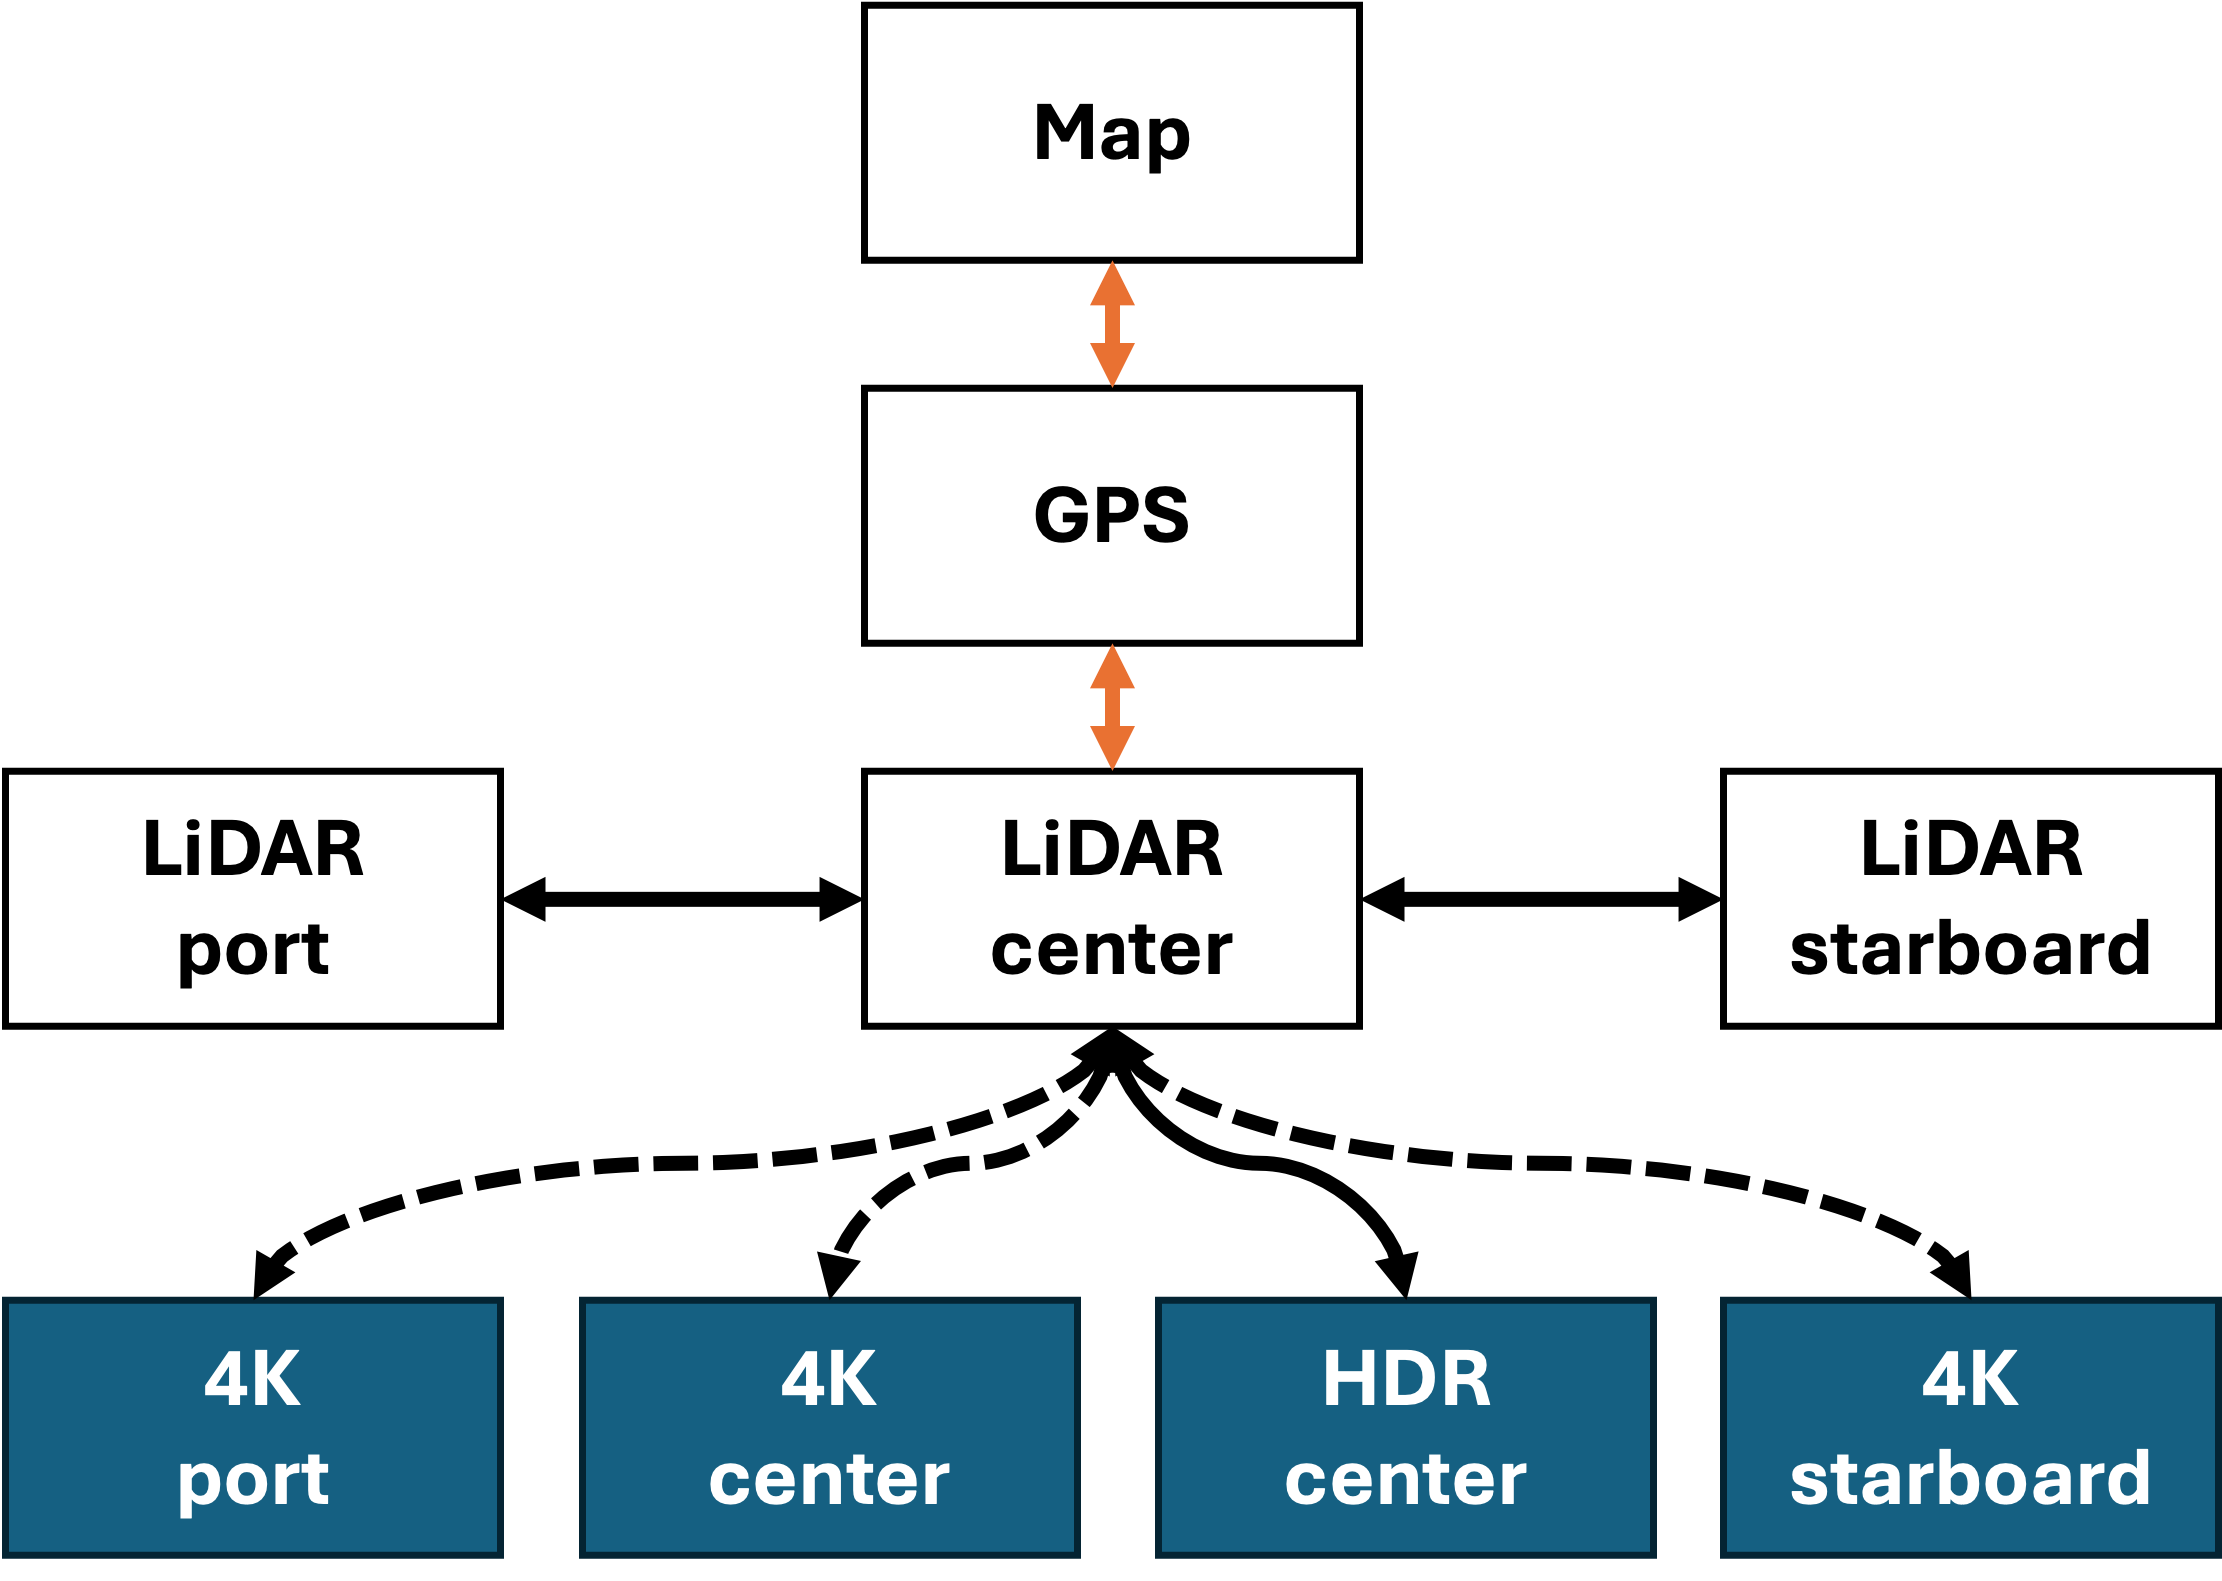
\includegraphics[width=0.7\linewidth]{Images/tf_tree.png}
%     \caption{Spatial transform tree between sensor reference frames onboard Minion.}
%     \label{fig:tf_tree}
% \end{figure}

% Because these transforms stack upon each other, they require calibration to achieve a level of precision to minimize compounding errors through the tree.
% Additionally, each sensor must maintain precise relative timing to one another to align the data from each sensor temporally.

% This section discusses the methods used to define these spatial transformations in \ref{spatial_calibration}, as well as temporal synchronization in \ref{time_sync}.

% \subsubsection{Camera Intrinsic Calibration} \label{HDR_intrinsic}

% Camera intrinsic parameters describe the internal geometry of a camera and define the mapping between three-dimensional coordinates in the camera frame and two-dimensional pixel locations in the image plane.  

\section{Sensor Calibration} \label{sec:calibration}

The multi-sensor perception suite described in the previous section integrates complementary sensing modalities: \ac{LiDAR} for spatial structure and cameras for visual context.
Each of these sensors measures the environment within its own local reference frame and according to its own internal clock.
To combine their observations into a consistent world model, the system must first be calibrated both spatially and temporally.

% Spatial calibration defines the transformations required to express all sensor measurements within a unified coordinate framework.
For the Minion platform, each sensor is rigidly mounted and assigned a reference frame within the overall transform hierarchy. 
The extrinsic calibration process involves estimating the rotation and translation between each sensor, and is represented by an arrow in Figure~\ref{fig:tf_tree}.
An additional intrinsic calibration must be performed for the camera sensors represented in blue.
Intrinsic calibration determines the optical characteristics of each camera, including focal length, principal point location, and lens distortion coefficients, as described in Section~\ref{spatial_calibration}.

For the Minion platform, all sensors are rigidly mounted and assigned reference frames within a unified transform hierarchy.
Spatial calibration establishes the geometric relationships among these frames by estimating the rotation and translation between sensor frames, represented by the arrows in Figure~\ref{fig:tf_tree}.  
Intrinsic calibration is also required for the visible-spectrum cameras (shown in blue), determining the internal optical parameters such as focal length, principal point location, and lens distortion. %, as detailed in Section~\ref{sec:HDR_calib}.
Time synchronization is similarly structured, with a master clock distributed over the network to subsystems and sensors to ensure that data acquired across sensor modalities remain temporally aligned.

Within this framework, the port and starboard Livox units are first registered to the center Livox reference frame before their point clouds are merged into a single unified point cloud.  
This consolidated LiDAR frame is then related to the HDR camera frame through an additional extrinsic transform, allowing three-dimensional LiDAR points $(x, y, z)$ to be projected onto the two-dimensional image plane $(u, v)$ using the camera’s intrinsic parameters.  
Finally, all perception data are kept in sync and expressed in the global map frame defined through the time, location, and orientation provided by the \ac{GPS}.

Section \ref{spatial_calibration} provides the methods used for intrinsic camera calibration, extrinsic calibration between the camera and LiDAR sensors, and between the individual LiDAR units. 
This is followed by a discussion of the time synchronization methods implemented across the network, with special detail provided to the timestamps applied to video frames in section \ref{time_sync}
Finally, the resulting spatial calibration accuracy and temporal alignment obtained are discussed in section \ref{time_sync}.

% % focuses on three primary calibration tasks.
% % First, the intrinsic parameters of the HDR camera are estimated, followed by the extrinsic alignment between the HDR camera and the center Livox reference frame.
% % Finally, the three Livox sensors are registered to one another to produce a unified LiDAR coordinate frame.
% % The calibration methods and corresponding results for each step are presented in the following subsections.

% % A rigid-body transformation $\mathbf{T}_{A}^{B}$ is used to move from reference frame $A$ to $B$

% % \begin{equation}
% %     \begin{bmatrix}
% %         \mathbf{R}_{A}^{B} & \mathbf{t}_{A}^{B} \\
% %             0 & 1
% %     \end{bmatrix},
% % \end{equation}
% % where $\mathbf{R}_{A}^{B}$ is a $3\times3$ rotation matrix and $\mathbf{t}_{A}^{B}$ is a translation vector defining the pose of frame $B$ relative to frame $A$.
% % Therefore, a set of points in reference frame $A$ ($_{A}\mathbf{P}$) can be expressed in reference frame $B$ ($_{B}\mathbf{P}$) through 
% % \begin{equation}
% %     _{B}\mathbf{P} =
% %     \mathbf{R}_{A}^{B}_{A}\mathbf{P} + \mathbf{t}_{A}^{B}.
% % \end{equation}




% Spatial calibration establishes the geometric relationships among all sensing elements.
% It quantifies each sensor’s intrinsic parameters—those governing its internal projection or ranging model—and the extrinsic transformations that define the relative positions and orientations among all sensors within the platform.
% In this system, the global chain of spatial relationships is maintained through \ac{ROS}, linking coordinate frames from the inertial map frame through the \ac{GPS} to the center Livox unit, and finally to each camera, shown in Figure \ref{fig:tf_tree}.
% Accurate spatial calibration ensures that a point detected in a \ac{LiDAR} scan can be correctly projected onto the image plane or the map frame, enabling correspondence between geometric and visual detections for downstream fusion.
% % Section \ref{spatial_calibration} details the methods used to calibrate the system, as well as the results achieved.

% Temporal calibration aligns sensor data streams in time so that observations correspond to the same physical instant.
% Because each device maintains its own internal clock and sampling rate, even small offsets can introduce spatial error.
% % The steps taken to achieve temporal synchronization and the results achieved are provided in section \ref{time_sync}.

% Spatial calibration methods, including camera intrinsic and extrinsic estimation and multi-\ac{LiDAR} registration, are presented in Section~\ref{spatial_calibration}, followed by the temporal synchronization framework in Section~\ref{time_sync}.
% Each section details both the methods employed and the resulting calibration accuracy achieved.

\begin{figure}[htbp]
    \centering
    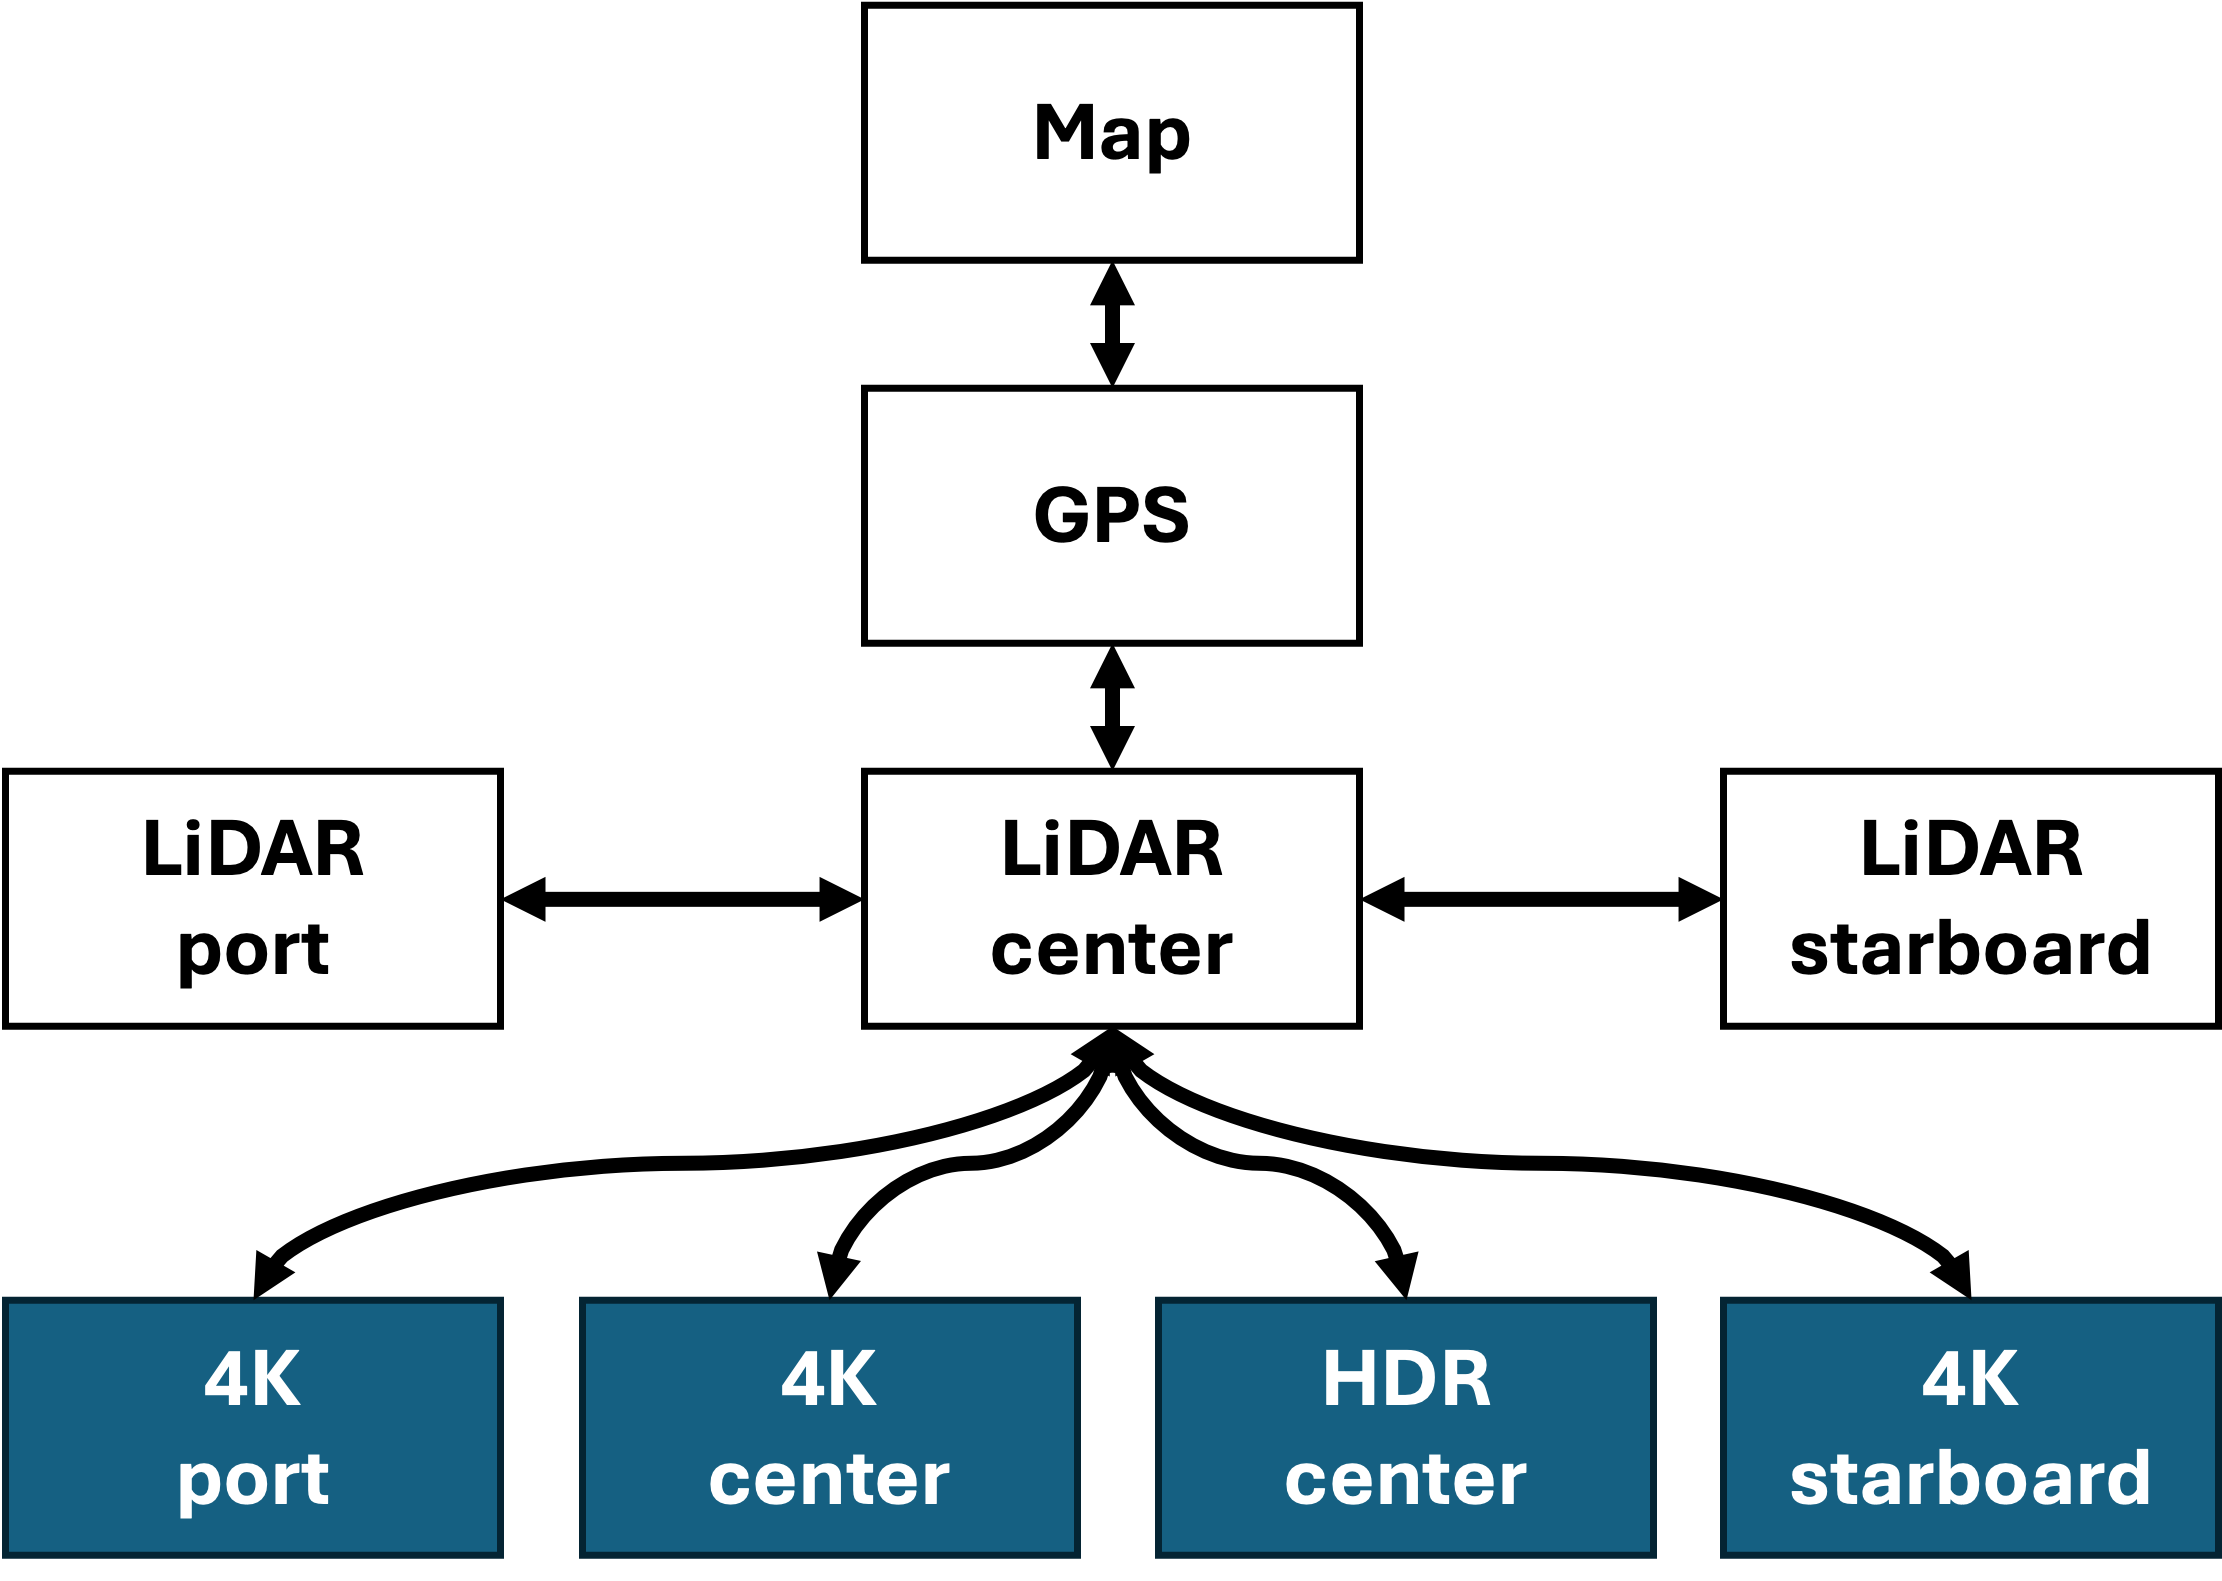
\includegraphics[width=0.7\linewidth]{Images/tf_tree_1.png}
    \caption{Spatial transform hierarchy for the perception system sensors onboard Minion.}
    \label{fig:tf_tree}
\end{figure}

%%%%%%%%%%%%%%%%%%%%%%%%%%%%%%%%%%%%%%%%%%%%%%%%%%%%%%%%%%%%%%%%%%%%
\subsection{Spatial Calibration} \label{spatial_calibration}

Before the data from the camera and \ac{LiDAR} sensors can be combined, each device needs to be spatially calibrated through extrinsic and intrinsic transforms.
Calibration between the two sensors begins by determining the camera's intrinsic parameters so that the LiDAR data can be accurately projected onto the image plane.

\subsubsection{Camera Intrinsics} \label{camera_intrinsics}

Camera intrinsic parameters define the internal geometry of the camera and describe how three-dimensional points in the camera coordinate frame are projected onto two-dimensional pixel locations in the image plane.  
They are governed by the optical path of light through the lens and onto the image sensor, and together they determine how spatial measurements are mapped into image coordinates.  
For modeling purposes, the intrinsic geometry can be separated into an idealized projection model and a lens distortion model.

Under the pinhole camera model, the projection of a world point onto the image plane is defined by the intrinsic matrix %$\mathbf{K}$:

\begin{equation}
    \mathbf{K} = 
    \begin{bmatrix}
        f_x & s & c_x \\
        0 & f_y & c_y \\
        0 & 0 & 1
    \end{bmatrix},
\end{equation}

where $(f_x, f_y)$ are the focal lengths along the primary axes expressed in pixels, $(c_x, c_y)$ is the pixel location where the optical axis intersects the image sensor (the principal point), and $s$ is the skew factor between the image’s horizontal and vertical axes (typically $s = 0$ for modern sensors with square pixels).

Real cameras deviate from this ideal projection model due to optical distortion from their lens.  
Light passing through the outer regions of the lens experiences more diffraction than light near the optical axis, resulting in a radial distortion.
This causes straight lines in the scene to appear curved within the image frame, an effect that becomes more pronounced with wide-angle or “fish-eye” lenses.  
This distortion assumes rotational symmetry about the optical axis, and is modeled using a polynomial expansion with coefficients $k_1$, $k_2$, and $k_3$ as
\begin{equation}
    \begin{split}
        x' &= x_n(1 + k_1 r^2 + k_2 r^4 + k_3 r^6), \\
        y' &= y_n(1 + k_1 r^2 + k_2 r^4 + k_3 r^6),
    \end{split}
\end{equation}

where $(x', y')$ are the distorted image coordinates of pin-hole camera model coordinates $(x_n, y_n)$, and $r$ is the radial distance from the optical center (principal point), given by $r = \sqrt{x_n^2 + y_n^2}$. 

Although this simplified radial model does not account for asymmetric or off-axis distortions arising from optical misalignment, such effects are typically negligible in high-quality camera systems.
However, even when the manufacturer provides intrinsic parameters, calibration remains necessary to achieve sub-pixel accuracy when projecting LiDAR points onto the image frame.

\subsubsection{Intrinsic Calibration} \label{intrinsic_calib}

To estimate a camera's intrinsic parameters, a calibration target with known geometric dimensions must be imaged from multiple positions and orientations within the camera’s field of view.  
A planar checkerboard pattern is widely adopted for this purpose due to its regular pattern of high-contrast corners, which can be reliably located using gradient-based corner detection algorithms such as the Harris method.  
These intersections provide multiple, evenly distributed feature points that enable calibration software to compute statistically optimal intrinsic parameters across a set of calibration images.

For effective calibration, the sequence of captured images should include dozens of images with the target placed at varying depths, orientations (roll, pitch, and yaw), and positions that cover the full field of view at distances representative of operational conditions.
Additionally, the checkerboard should have physical dimensions comparable to the scale of objects expected in the environment. This ensures that the selected camera has the pixel density necessary (as described in Section~\ref{camera_selection}) to resolve the checkerboard corners.
These practices ensure that the estimated intrinsic parameters are well-constrained and remain valid across the camera’s operational envelope.


\subsubsection{Extrinsic Calibration} \label{extrinsic_tform}
% \subsubsection{Camera–LiDAR Extrinsic Calibration} \label{extrinsic_calib}

% the LiDAR and camera reference frames, consisting of a rotation matrix $\mathbf{R}_{C}^{L}$ and translation vector $\mathbf{t}_{C}^{L}$ that together form the homogeneous transformation $_{C}^{L}\mathbf{T}$.  

Extrinsic calibration defines the rigid-body transformation between two reference frames.
The transformation from frame $A$ to frame $B$ is represented as
\begin{equation}
    _{B}^{A}\mathbf{T} =
    \begin{bmatrix}
        _{B}^{A}\mathbf{R} & _{B}^{A}\mathbf{t} \\
        \mathbf{0}^\mathrm{T} & 1
    \end{bmatrix},
\end{equation}

where $\mathbf{R}_{B}^{A} \in \mathbb{R}^{3\times3}$ is the rotation matrix describing the orientation of frame $A$ relative to frame $B$, and $_{B}^{A}\mathbf{t} \in \mathbb{R}^{3}$ is the translation vector locating the origin of frame $A$ with respect to frame $B$.  
The notation convention used here follows that the subscript denotes the destination frame, and the superscript denotes the source frame.

A point $_{A}\mathbf{P}$ expressed in frame $A$ can therefore be transformed into frame $B$ as

\begin{equation}
    _{B}\mathbf{P} =
    _{B}^{A}\mathbf{R} _{A}\mathbf{P} + _{B}^{A}\mathbf{t}.
\end{equation}

This formulation provides a unified framework for expressing all spatial relationships among the platform’s sensors, allowing transformations to be composed sequentially through the transform tree illustrated in Figure~\ref{fig:tf_tree}.

% This transformation provides the geometric foundation for projecting three-dimensional LiDAR points into the two-dimensional camera image frame using the intrinsic parameters defined in Section~\ref{camera_intrinsics}.

This transformation enables points measured in the LiDAR frame to be accurately projected into the camera image, allowing geometric features to be aligned with their visual counterparts.

\subsubsection{Camera–LiDAR Extrinsic Calibration} \label{camLidar_calib}

The calibration process begins by co-locating a planar checkerboard target within the LiDAR point cloud and the camera image.  
The physical extents of the checkerboard observed in the LiDAR frame ($X_L, Y_L, Z_L$) are matched to the corresponding pixel locations in the image frame ($u,v$), yielding an approximate estimate of the relative orientation and position between the two sensors.  
This initial alignment provides a coarse estimate of $_{C}^{L}\mathbf{T}$ sufficient for projecting LiDAR points into the image plane with moderate accuracy.

\begin{figure}[htbp]
\centering
\makebox[\textwidth][c]{
    \begin{subfigure}[t]{0.44\textwidth}
        \centering
        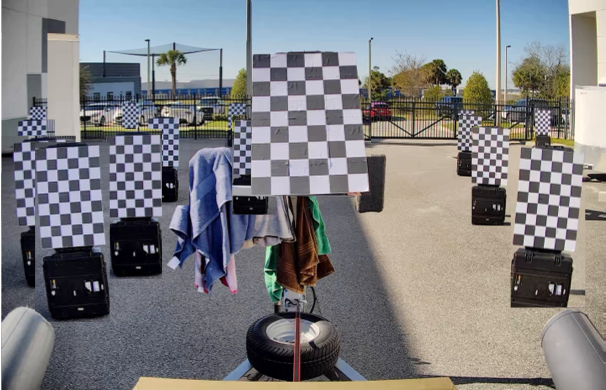
\includegraphics[width=\textwidth]{Images/checkerboard.png}
        \caption{Composite image of multiple target checkerboard locations.}
        \label{fig:checkerboard}
    \end{subfigure}
    \hspace{2em} % horizontal spacing between them
    \begin{subfigure}[t]{0.44\textwidth}
        \centering
        \includegraphics[width=\textwidth]{Images/LiDAR_calib.png}
        \caption{Composite location of checkerboards within the LiDAR reference frame.}
        \label{fig:LiDAR_calib}
    \end{subfigure}
}
\caption{Composite images showing the location of the target checkerboard in multiple locations as a representative sample of the intrinsic calibration for the HDR camera (left) and a composite of the same calibration checkerboards spatially located within the LiDAR reference frame (right). Red dots represent the corner points of the checkerboard transformed into the LiDAR reference frame with initial extrinsic calibration values.}
\label{fig:camLidar_calib}
\end{figure}

% \begin{equation}
%     \begin{bmatrix}
%         \mathbf{R}_{A}^{B} & \mathbf{t}_{A}^{B} \\
%             0 & 1
%     \end{bmatrix},
% \end{equation}
% where $\mathbf{R}_{A}^{B}$ is a $3\times3$ rotation matrix and $\mathbf{t}_{A}^{B}$ is a translation vector defining the pose of frame $B$ relative to frame $A$.
% Therefore, a set of points in reference frame $A$ ($_{A}\mathbf{P}$) can be expressed in reference frame $B$ ($_{B}\mathbf{P}$) through 
% \begin{equation}
%     _{B}\mathbf{P} =
%     \mathbf{R}_{A}^{B}_{A}\mathbf{P} + \mathbf{t}_{A}^{B}.
% \end{equation}
A mapping of three-dimensional points to pixel coordinates in the distorted image frame is provided in Appendix \ref{img_tform}.

This initial calibration is easily performed in packages designed for LiDAR calibration, such as the MATLAB LiDAR Calibration tool \cite{matlab_calibration}.
Further refinement is achieved through manual inspection of iterative changes to the extrinsic values, or through an \ac{ICP} method.

The \ac{ICP} algorithm adjusts the transformation parameters in small increments to minimize the distance between corresponding features observed by both sensors when projected into a shared reference frame.
In this application, ICP minimizes the point-to-plane error between the checkerboard corners projected from the camera and the planar points corresponding to the checkerboard surface in the LiDAR point cloud.

Alternatively, manual refinement can be conducted by visually matching large-scale environmental features—such as walls, trees, fences, or other clearly defined structures—present in both modalities.  
This final adjustment ensures that the extrinsic transformation achieves sub-degree rotational accuracy and centimeter-level translation precision, suitable for sensor fusion and object-detection applications.

% \subsubsection{HDR Calibration} \label{sec:HDR_calib}

% A three-dimensional point $\mathbf{P}_c = [X_c, Y_c, Z_c]^T$ expressed in the camera reference frame is projected onto the image plane using the intrinsic matrix $\mathbf{K}$ and the normalized coordinates $(x', y')$ obtained from the distortion model:

% \begin{equation}
% \begin{bmatrix}
% u \\ v \\ 1
% \end{bmatrix}
% =
% \mathbf{K}
% \begin{bmatrix}
% x' \\ y' \\ 1
% \end{bmatrix}
% =
% \begin{bmatrix}
% f_x & s & c_x \\
% 0   & f_y & c_y \\
% 0   & 0   & 1
% \end{bmatrix}
% \begin{bmatrix}
% \dfrac{X_c}{Z_c}(1 + k_1 r^2 + k_2 r^4 + k_3 r^6) \\[1.0em]
% \dfrac{Y_c}{Z_c}(1 + k_1 r^2 + k_2 r^4 + k_3 r^6) \\[1.0em]
% 1
% \end{bmatrix},
% \label{eq:projection_model}
% \end{equation}

% where $(u, v)$ are the distorted pixel coordinates in the image plane and $(X_c, Y_c, Z_c)$ are the point coordinates in the camera frame.  
% This formulation explicitly combines the pinhole projection with the radial distortion model, allowing spatial points captured by a \ac{LiDAR} or other 3D sensor to be accurately projected onto the camera image for correspondence and fusion analysis.

% --



% \[
% \mathbf{T}_{A}^{B} =
% \begin{bmatrix}
% \mathbf{R}_{A}^{B} & \mathbf{t}_{A}^{B} \\
% 0 & 1
% \end{bmatrix},
% \]
% where $\mathbf{R}_{A}^{B}$ is a $3\times3$ rotation matrix and $\mathbf{t}_{A}^{B}$ is a translation vector defining the pose of frame $B$ relative to frame $A$.

% where $(f_x, f_y)$ are the focal lengths expressed in pixels, $(c_x, c_y)$ is the \textit{principal point}, the pixel location where the optical axis intersects the image sensor, and $s$ is the skew factor between the image’s horizontal and vertical axes (typically $s = 0$ for modern sensors with square pixels).

% Lenses introduce optical distortion that deviates from the pinhole camera model.  
% Radial distortion, caused by lens curvature, bends straight lines in the scene and results in a barrel- or bubble-like appearance in the captured image.  
% Lenses with ultra-wide fields of view, known as fish-eye lenses, exhibit this effect most prominently.  
% The distortion is modeled by a polynomial function with coefficients $k_1$, $k_2$, and $k_3$:

% \begin{equation}
%     \begin{split}
%         x_d &= x_n(1 + k_1 r^2 + k_2 r^4 + k_3 r^6), \\
%         y_d &= y_n(1 + k_1 r^2 + k_2 r^4 + k_3 r^6),
%     \end{split}
% \end{equation}

% where $(x_d, y_d)$ are the distorted coordinates and $r$ is the radial distance from the principal point, defined as $r = \sqrt{x_n^2 + y_n^2}$.  
% The normalized image coordinates $(x_n, y_n)$ are obtained by removing the effects of focal length and principal point from the pixel coordinates $(x_p, y_p)$:

% \begin{equation}
%     x_n = \frac{x_p - c_x}{f_x}, \qquad
%     y_n = \frac{y_p - c_y}{f_y}.
% \end{equation}

% These normalized coordinates describe a unitless position on the idealized image plane, centered on the optical axis and expressed in focal-length units rather than pixels.  
% Accurate modeling and correction of this distortion are essential for projecting three-dimensional LiDAR points into the camera frame or for rectifying images onto a flat plane prior to sensor fusion.  
% Although some manufacturers publish nominal intrinsic parameters, in-situ calibration is required to compensate for manufacturing tolerances, lens alignment, and mounting variations, enabling the sub-pixel accuracy necessary for precision multi-sensor perception.

% % \subsubsection{Calibration Methodology}

% Camera intrinsic calibration employs the standard checkerboard pattern approach, widely adopted in computer vision due to the availability of mature implementations in OpenCV and MATLAB.
% A planar checkerboard pattern with known physical dimensions serves as the calibration target.
% The pattern consists of alternating black and white squares arranged in a grid, with corner points providing precisely-defined feature locations for correspondence establishment.
% For the Minion platform, I constructed a calibration target with an $8 \times 5$ checkerboard grid with 100 mm square spacing, resulting in total board dimensions of 700 mm $\times$ 400 mm.
% The squares were hand-marked using calipers and compass for accuracy, then painted with high-contrast black and white marine paint suitable for outdoor use.

% Calibration images are captured with the checkerboard pattern positioned at multiple locations and orientations throughout the camera field of view.
% Images must include the calibration pattern at varying depths, angles (varying roll, pitch, and yaw), and positions within the frame (center, edges, and corners).
% For maritime perception applications where objects may appear from 0.5 to 60 meters, the calibration dataset should span a similarly wide distance range to ensure intrinsic parameters are well-constrained across operational conditions.
% I collected 40 calibration images per camera, providing sufficient geometric diversity for robust parameter estimation.
% The camera focus was locked at the operational setting used during data collection, and exposure was adjusted to ensure clear visibility of checkerboard corners.
% Calibration was performed indoors with controlled lighting to avoid shadows and glare that would degrade corner detection.

% MATLAB's Camera Calibration application was used to estimate intrinsic parameters \cite{matlab_calibration} \cite{matlab_vision}.
% The tool implements Zhang's method, which identifies the intersecting corner points formed by the checkerboard squares and measures their distances in pixels.
% This information is cross-referenced with the physical dimensions of the checkerboard pattern.
% The algorithm estimates the camera's intrinsic properties by minimizing the reprojection error between the observed checkerboard patterns and projected points through a pinhole camera model with distortion correction.

% % \subsubsection{Calibration Results} \label{HDR_intrinsic_result}

% The intrinsic calibration of the Leopard Imaging IMX490 \ac{HDR} camera (2880 $\times$ 1860 pixels, 65° field of view) demonstrated excellent quality with a mean reprojection error of 0.158 pixels and \ac{RMS} error of 0.200 pixels.
% The calibration dataset consisted of 40 images containing a total of 1,600 checkerboard corner keypoints spanning distances from 3.1 to 42.8 meters—more than an order of magnitude in range.
% This wide distribution ensures the intrinsic parameters are well-constrained across operational conditions typical of maritime perception scenarios.

% The calibrated focal lengths were $f_x = 2611.16 \pm 34.51$ pixels and $f_y = 2604.73 \pm 31.65$ pixels, exhibiting near-identical values with a difference of only 6.43 pixels (0.25%).
% This similarity indicates minimal aspect ratio distortion and is well within the uncertainty bounds.
% The low relative errors (1.32\% and 1.21\%, respectively) indicate well-constrained estimates.
% The principal point was located at $(c_x, c_y) = (1359.09 \pm 14.59, 966.39 \pm 18.93)$ pixels, offset from the geometric image center by approximately 81 pixels horizontally and 36 pixels vertically.
% This offset is typical for real cameras due to manufacturing tolerances, and the uncertainty of less than 20 pixels represents less than 0.7\% of the image width.
% The skew parameter was measured as $s = 5.02 \pm 1.18$, near-zero as expected for modern sensors with nearly perpendicular pixel array axes.

% The radial distortion coefficients were $k_1 = -0.349155 \pm 0.007614$ and $k_2 = +0.141328 \pm 0.008625$.
% The negative $k_1$ indicates strong barrel distortion characteristic of wide-angle lenses, while the positive $k_2$ provides compensatory pincushion correction.
% This combination is typical for the 65° field of view lens employed by the IMX490 camera, with $k_1$ dominating the distortion profile near image edges.
% Tangential distortion coefficients were minimal ($p_1 = -0.000906 \pm 0.000950$, $p_2 = +0.003116 \pm 0.000679$), indicating good optical alignment with slight horizontal lens decentering suggested by the larger $p_2$ value.

% The sub-pixel reprojection accuracy represents approximately 0.005\% of the image width, demonstrating excellent calibration quality.
% The low standard deviation of 0.123 pixels indicates uniform quality across all calibration images, and the maximum error of 0.717 pixels is acceptably below the 1-pixel threshold.
% The tight error distribution suggests the Brown-Conrady distortion model with two radial coefficients and two tangential coefficients adequately captures the lens characteristics.
% Using the calibrated focal length, the angular resolution is 0.0219 degrees per pixel horizontally and 0.0220 degrees per pixel vertically.
% The reprojection errors translate to metric uncertainties that scale with distance: at 5 meters, the mean positional error is $\pm$1.5 mm; at 10 meters, $\pm$3.0 mm; at 20 meters, $\pm$6.1 mm; and at 40 meters, $\pm$12.1 mm.
% These accuracies meet or exceed requirements for maritime object detection and sensor fusion research applications, where buoy detection at 5-20 meters requires positional errors below 5 cm.

% % \subsubsection{Camera Extrinsic Calibration}

% Extrinsic calibration determines the six-degree-of-freedom transformation (three-dimensional translation and three-dimensional rotation) relating each camera's coordinate system to a common platform reference frame.
% The transformation from camera coordinates to platform coordinates combines rotation and translation:

% \begin{equation*}
%     \mathbf{p}_{\text{platform}} = \mathbf{R}_{\text{cam}}^{\text{plat}} \mathbf{p}_{\text{camera}} + \mathbf{t}_{\text{cam}}^{\text{plat}}
% \end{equation*}

% where $\mathbf{R}_{\text{cam}}^{\text{plat}}$ is the $3 \times 3$ rotation matrix, $\mathbf{t}_{\text{cam}}^{\text{plat}}$ is the $3 \times 1$ translation vector, $\mathbf{p}_{\text{camera}}$ is a point in camera coordinates, and $\mathbf{p}_{\text{platform}}$ is the same point in platform coordinates.

% % \subsubsection{Coordinate Frame Definitions}

% The multi-sensor platform employs several coordinate frames that must be precisely related.
% The camera frame has its origin at the camera's optical center, with the Z-axis pointing along the optical axis into the scene, X-axis pointing right, and Y-axis pointing down, following the standard computer vision convention.
% The \ac{LiDAR} frame has its origin at the primary \ac{LiDAR} sensor location, with coordinate axes defined by the sensor manufacturer's specification (Z-up, X-forward for Livox Horizon sensors).
% The platform frame is a vessel-fixed reference frame with origin at a convenient mechanical datum and axes aligned with vessel principal directions (forward, starboard, down).
% The world frame is an inertial reference frame defined by the \ac{GPS}/\ac{INS} system, with position in WGS84 geographic coordinates and orientation relative to true north and local gravity.

% % \subsubsection{Calibration Approach}

% Camera-to-platform extrinsic calibration employs a target-based approach where the same checkerboard pattern used for intrinsic calibration serves as the extrinsic calibration target.
% The checkerboard is placed at a known, measurable location in the platform frame, and the camera captures an image of the pattern.
% Using the intrinsically-calibrated parameters to detect corner locations, OpenCV's \texttt{solvePnP} algorithm estimates the camera pose relative to the checkerboard pattern.
% The known checkerboard-to-platform transformation is combined with the estimated camera-to-checkerboard transformation to obtain camera-to-platform extrinsics:

% \begin{equation*}
%     \mathbf{T}_{\text{cam}}^{\text{plat}} = \mathbf{T}_{\text{target}}^{\text{plat}} \cdot \mathbf{T}_{\text{cam}}^{\text{target}}
% \end{equation*}


% where $\mathbf{T}$ denotes $4 \times 4$ homogeneous transformation matrices combining rotation and translation.

% An alternative and complementary approach directly calibrates the camera-to-\ac{LiDAR} transformation by leveraging the fact that \ac{LiDAR} provides precise distance measurements to target features.
% A calibration board with retroreflective markers or distinctive geometric features clearly visible in both camera images and \ac{LiDAR} point clouds enables identification of corresponding feature points in camera images (pixel coordinates) and \ac{LiDAR} point clouds (3D coordinates).
% The optimization solves for rotation and translation that minimize reprojection error when \ac{LiDAR} points are transformed to the camera frame and projected via the intrinsic model:

% \begin{equation*}
%     E = \sum_{i=1}^{N} \left\| \mathbf{u}_i - \pi(\mathbf{K}, \mathbf{R}, \mathbf{t}, \mathbf{X}_i) \right\|^2
% \end{equation*}

% where $\mathbf{u}_i$ are observed 2D feature locations in the image, $\mathbf{X}_i$ are corresponding 3D points in the \ac{LiDAR} frame, $\pi()$ is the projection function applying rotation $\mathbf{R}$, translation $\mathbf{t}$, and camera matrix $\mathbf{K}$, and $N$ is the number of correspondences.

% For the Minion platform calibration, I employed a combined approach.
% Multiple checkerboard locations were captured in both camera images and \ac{LiDAR} scans.
% From camera images, 3D checkerboard corners were extracted using the intrinsic calibration parameters.
% For each checkerboard location, a 5-second aggregated \ac{LiDAR} scan provided sufficient point density to clearly resolve the planar target surface.
% All camera corners were aggregated into a single point cloud, and all \ac{LiDAR} scans from different board locations were combined.
% Manual point-pair selection in CloudCompare software enabled registration between the camera-derived corner point cloud and the \ac{LiDAR}-derived surface observations.

% One critical observation during camera-to-\ac{LiDAR} calibration was that checkerboard dimensions appeared to increase with distance in image space, suggesting residual intrinsic calibration errors.
% To correct for this, an affine transformation (incorporating translation, rotation, scale, and shear) was used instead of a purely rigid transformation (translation and rotation only).
% This affine approach compensates for minor intrinsic calibration errors and improves alignment, particularly for far-target observations.
% Following the methodology established by \cite{thompson2023}, this affine calibration approach ensures geometric consistency across the operational range of the sensors.

% During the calibration process, I discovered that the \ac{HDR} camera is angled down at 8 degrees from the level plane of the camera enclosure, matching the pitch angle of the center Livox \ac{LiDAR} unit.
% This geometric alignment simplifies the extrinsic transformation by ensuring both sensors have similar downward-looking orientations, reducing the magnitude of rotational corrections needed in the camera-to-\ac{LiDAR} transform.

% % \subsubsection{Calibration Validation}

% Extrinsic calibration quality is validated through multiple criteria.
% Reprojection error analysis projects 3D calibration points through the estimated extrinsics and intrinsics, computing pixel-space error:

% \begin{equation*}
%     \text{RMS reprojection error} = \sqrt{\frac{1}{N}\sum_{i=1}^{N} \left\| \mathbf{u}_i - \hat{\mathbf{u}}_i \right\|^2}
% \end{equation*}

% Acceptable error for well-calibrated systems is less than 1-2 pixels.
% Visual overlay inspection confirms calibration quality by overlaying \ac{LiDAR} point clouds on camera images using the estimated extrinsics and intrinsics.
% Visual inspection verifies that \ac{LiDAR} returns on vertical structures such as poles and building edges align with image features, that distances from camera to \ac{LiDAR}-observed objects match expected geometry, and that systematic offsets or rotational misalignments are absent.

% % \subsubsection{LiDAR Extrinsic Calibration}

% The Minion platform employs three Livox Horizon \ac{LiDAR} units positioned to provide overlapping forward-facing coverage.
% Extrinsic calibration establishes the geometric relationships between these three sensors and between the unified \ac{LiDAR} reference frame and the platform coordinate system, enabling aggregation of point clouds from multiple sensors and projection of \ac{LiDAR} observations onto camera images.

% % \subsubsection{Calibration Architecture}

% The multi-\ac{LiDAR} configuration requires two levels of extrinsic calibration.
% First, \ac{LiDAR}-to-\ac{LiDAR} calibration determines the six-degree-of-freedom transformations relating each of the three Livox Horizon units to a common \ac{LiDAR} reference frame, enabling merging of point clouds from all three sensors into a unified coordinate system.
% Second, \ac{LiDAR}-to-platform calibration establishes the transformation from the unified \ac{LiDAR} reference frame to the vessel platform reference frame, enabling integration with other sensors and transformation to world coordinates during vehicle motion.

% The three Livox Horizon units are designated as left, center, and right based on their positions in the forward-facing array.
% The center sensor is selected as the reference, with left and right sensors calibrated relative to center.
% The Livox Horizon sensors provide a significant calibration advantage: extrinsic parameters can be written to onboard non-volatile memory, configuring the sensors to automatically apply coordinate transformations before broadcasting point cloud data.
% This factory-configured capability simplifies downstream processing by presenting pre-registered point clouds to the perception pipeline, eliminating the need for software-based point cloud registration at runtime.

% % \subsubsection{LiDAR-to-LiDAR Calibration Methodology}

% A planar calibration target with high \ac{LiDAR} reflectivity serves as the reference geometry.
% The target is positioned such that all three sensors observe it simultaneously, enabling correspondence-based calibration.
% For the Minion platform, the walls and right-angle corners of the research laboratory provided large flat surfaces suitable for plane-based calibration and cross-checking of alignment quality.

% Livox provides proprietary calibration software that automates the plane-based calibration procedure.
% The tool captures point clouds from all three sensors simultaneously, performs automatic plane segmentation, estimates rotation and translation parameters, validates calibration quality via residual error metrics, and uploads calibration parameters to sensor onboard memory.
% Dense point clouds acquired during calibration assist the alignment process, with the Livox software allowing real-time editing of extrinsic values and making alignment of large flat surfaces straightforward.
% The Minion platform calibration, originally performed by \cite{thompson2023}, utilized the Livox calibration tool following manufacturer procedures.

% The calibration methodology follows an \ac{ICP} approach.
% For data collection, 10-second scans from each \ac{LiDAR} sensor are captured while the platform is stationary, creating a single large aggregated scan per sensor in a cluttered static environment.
% The \ac{ICP} algorithm aligns the port and starboard sensor scans to the center sensor scan by iteratively calculating the closest points between two point clouds, calculating the registration (rotation $\mathbf{R}$ and translation $\mathbf{T}$), applying the registration, evaluating the mean-square error $E = \sum \|\mathbf{p}_{\text{target}} - \mathbf{p}_{\text{source}} \cdot \mathbf{R} - \mathbf{T}\|^2$, and repeating until $E$ is below a threshold.
% The resulting corrections are applied to geometric mount assumptions.
% For example, the port \ac{LiDAR} calibration yielded rotation corrections of [0.006, 0.035, 0.060] radians (yaw, pitch, roll) and translation corrections of [0.051, 0.004, 0.001] meters.

% Calibration quality is validated through plane alignment residuals.
% After applying estimated transformations, points from all three sensors observing the same plane should lie in a common plane with minimal scatter:

% \begin{equation*}
%     \sigma_{\text{residual}} = \sqrt{\frac{1}{N}\sum_{i=1}^{N} (n^T \mathbf{p}_i + d)^2}
% \end{equation*}

% where $n$ is the plane normal, $d$ is the plane offset, and $\mathbf{p}_i$ are the transformed points.
% Acceptable residual standard deviation is less than 5 mm for well-calibrated sensors at 5-10 meter range.
% Additional validation includes inspecting overlap regions where sensor fields of view overlap—the same physical features should produce closely aligned points from multiple sensors—and examining vertical edges such as poles and building corners, which should produce continuous linear features when point clouds from all three sensors are merged.
% Discontinuities or offsets at overlap boundaries indicate calibration errors.

% % \subsubsection{LiDAR-to-Platform Calibration}

% After establishing unified \ac{LiDAR} coordinates via sensor-to-sensor calibration, the \ac{LiDAR} reference frame must be related to the platform frame.
% The transformation from the center \ac{LiDAR} sensor to the platform origin can be determined via direct geometric measurement.
% A mechanical datum establishes the platform coordinate origin (for example, the vessel center of gravity or \ac{GPS} antenna mounting point).
% Physical measurement of the XYZ offset from platform origin to \ac{LiDAR} sensor origin using precision measurement tools such as calipers, laser distance meters, or coordinate measurement machines provides translation estimates.
% Angular orientation (roll, pitch, yaw) of the \ac{LiDAR} sensor relative to platform axes is determined using inclinometers or alignment jigs.
% This approach provides transformation estimates accurate to $\pm$10 mm in translation and $\pm$1° in rotation, typically sufficient for maritime perception applications where object dimensions are tens of centimeters to meters.

% The calibrated \ac{LiDAR}-to-platform extrinsics established by \cite{thompson2023} required no recalibration for the current research, as the sensor mounting remained mechanically stable between studies.
% However, camera extrinsic parameters are sensitive to mechanical changes and require recalibration if camera mounting hardware is adjusted or replaced, if vessel structural changes affect camera mounting location, after significant mechanical shock such as collision or hard grounding, or periodically for long-term deployments (for example, annually).

% % \subsubsection{Integration with ROS tf2 Framework}

% The Robot Operating System's \texttt{tf2} library maintains time-varying transformation trees between coordinate frames.
% Extrinsic calibration parameters are published as static transforms that relate sensor frames to the platform frame.
% The \texttt{tf2} framework automatically composes transformation chains, enabling queries such as "transform this \ac{LiDAR} point from \texttt{LiDAR\_frame} to \texttt{camera\_optical\_frame} at timestamp T" without manual transformation matrix multiplication.
% This capability is essential for the temporal aggregation methodology, which transforms \ac{LiDAR} points from sensor frame to platform frame using extrinsic calibration, then from platform frame to inertial world frame using \ac{GPS}/\ac{INS} pose at point acquisition time, accumulates points from multiple time steps in world frame, transforms aggregated points from world frame through platform frame to camera frame at image capture time, and finally projects to image pixels using camera intrinsics.

% Errors in \ac{LiDAR} extrinsics propagate through this transformation chain, causing spatial misalignment proportional to range and angular error.
% For example, a 1° rotation error produces approximately 17 mm lateral offset per meter of range—negligible at close range but significant for observations beyond 10 meters.
% The Livox Horizon's onboard calibration storage ensures that sensor-to-sensor transformations persist across power cycles and firmware updates, eliminating calibration drift that would occur with software-only transformation.

% % \subsubsection{Summary}

% The spatial calibration framework provides the complete geometric foundation necessary for accurate multi-modal sensor fusion.
% Camera intrinsic calibration achieves sub-pixel reprojection accuracy (0.158 $\pm$ 0.123 pixels) with well-constrained focal length, principal point, and distortion parameters across a wide operational range (3-43 meters).
% Camera extrinsic calibration establishes the six-degree-of-freedom transformation from camera frames to platform reference, validated through reprojection error analysis and visual overlay inspection.
% \ac{LiDAR} extrinsic calibration unifies three Livox Horizon point clouds into a common reference frame with sub-centimeter alignment at typical operating ranges and relates the \ac{LiDAR} reference frame to the platform coordinate system.
% The integration of these calibrations with the ROS \texttt{tf2} framework enables automated coordinate frame transformations essential for temporal aggregation and \ac{LiDAR}-camera projection, providing the spatial precision required for the object detection performance comparison analysis.

%%%%%%%%%%%%%%%%%%%%%%%%%%%%%%%%%%%%%%%%%%%%%%%%%%%%%%%%%%%%%%%%%%%%
\subsection{Temporal Calibration}\label{time_sync}

Multi-modal sensor fusion for object detection fundamentally requires accurate temporal alignment of observations from sensors operating with independent clocks and sampling at different rates.
The Minion platform employs a hierarchical temporal calibration architecture that distributes GPS-disciplined time from a single authoritative source through multiple computing platforms to all perception sensors, ensuring millisecond-level synchronization for camera observations and microsecond-level precision for LiDAR spatial measurements.
This three-tier synchronization system, employing GPS as the time authority, Network Time Protocol for coarse distribution, and IEEE 1588 Precision Time Protocol for fine synchronization, provides the temporal reference frame essential for rigorous cross-modal detection performance analysis.

The temporal calibration methodology addresses timing challenges specific to distributed embedded systems operating in maritime environments where internet connectivity is unavailable and GPS represents the sole external time reference.
Cameras and LiDAR sensors timestamp observations independently using local clocks, yet valid sensor fusion demands that all observations share a common temporal reference.
Without accurate time synchronization, a vessel traveling at 5 meters per second accumulates 5 millimeters of spatial misalignment for every millisecond of timing error, rendering temporal associations between camera frames and LiDAR scans unreliable for detection performance comparison.

The GPS-NTP-PTP cascaded synchronization architecture addresses accuracy requirements varying by sensor type.
Millisecond precision suffices for 10 Hz camera frame timestamps, while individual LiDAR laser returns require sub-millisecond accuracy to avoid spatial smearing during vehicle motion.
The hierarchical architecture exploits protocol characteristics matched to sensor needs: NTP provides simplicity and wide device compatibility for distributing time to computing platforms, while PTP achieves the microsecond-level precision demanded by spatial measurement sensors through hardware-timestamped network packets and symmetric delay compensation.

The synchronization infrastructure must accommodate operational constraints including dual redundant computing platforms requiring coordination to prevent conflicting time sources, automated startup verification to ensure synchronization establishment before data recording begins, and diagnostic capabilities enabling remote monitoring of synchronization quality during offshore operations.
Additionally, the video processing pipeline introduces systematic timing offsets between frames recorded locally on the camera enclosure computer and frames transmitted over the network to the primary computing platform, necessitating comprehensive temporal drift analysis and correction procedures to achieve frame-accurate temporal alignment.

%%%%%%%%%%%%%%%%%%%%%%%%%%%%%%%%%%%%%%%%%%%%%%%%%%%%%%%%%%%%%%%%%%%%
\subsubsection{Network Synchronization} \label{time_sync_lan}


\begin{figure}[htbp]
\centering
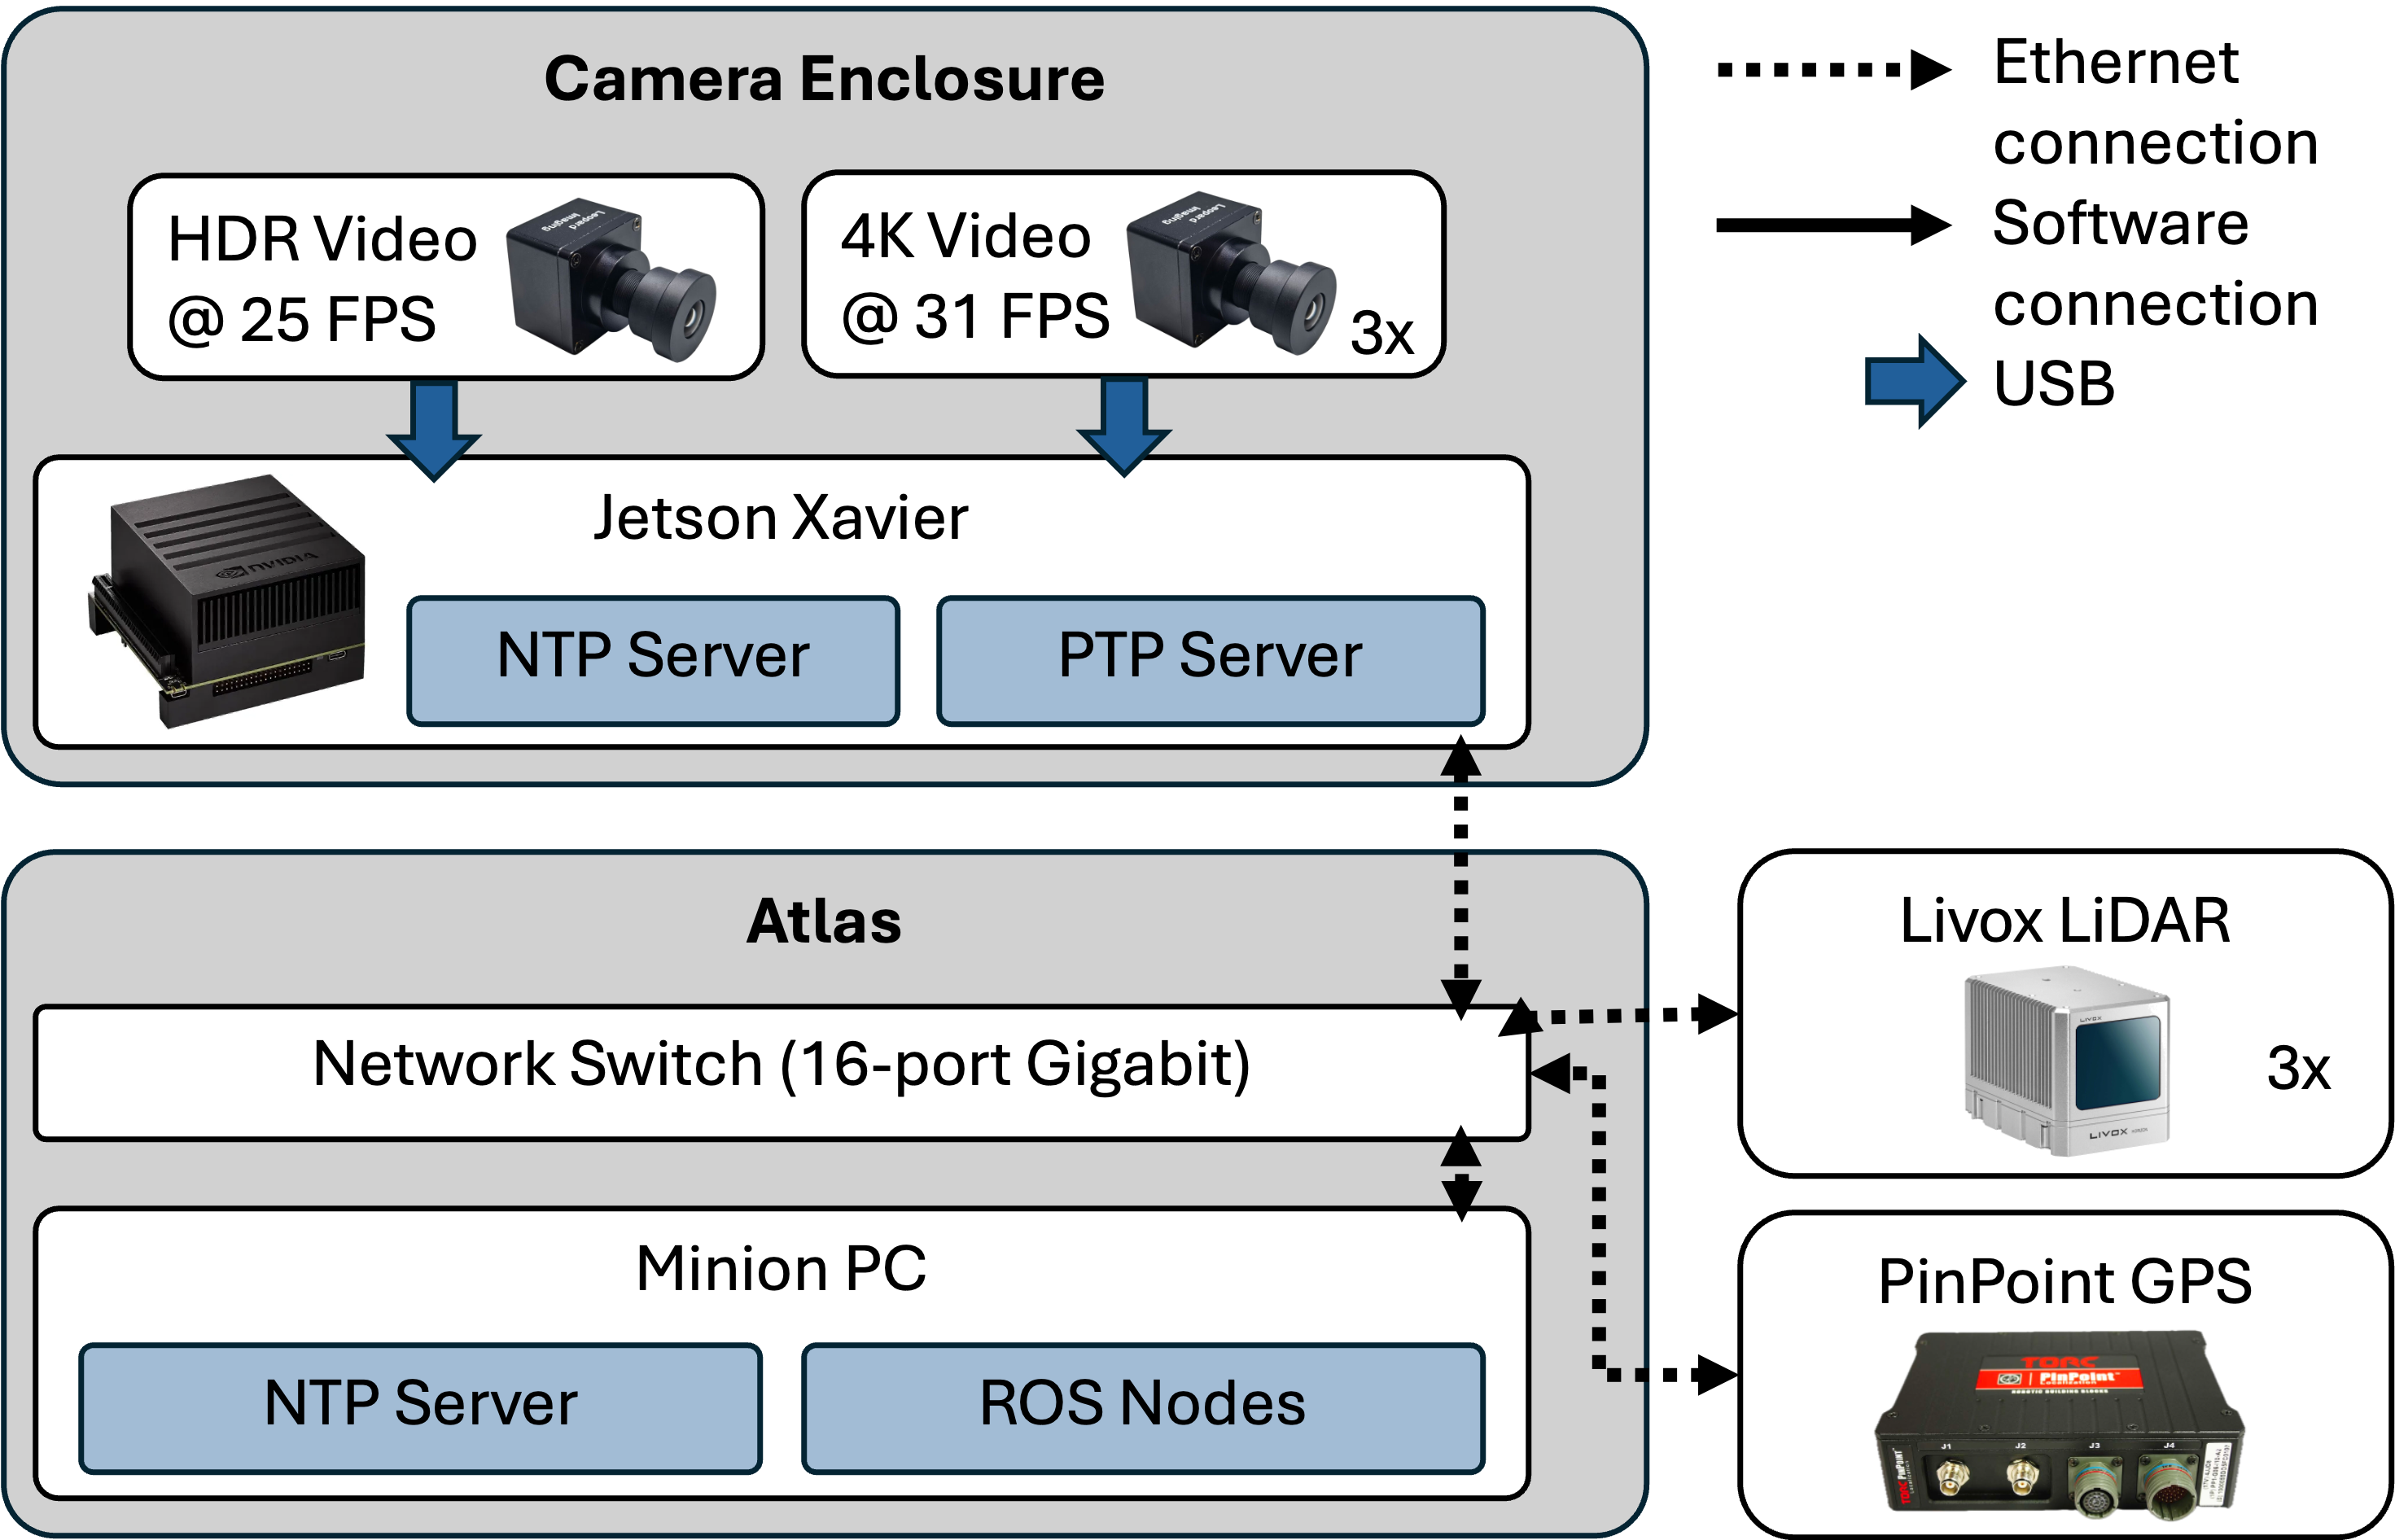
\includegraphics[width=0.8\textwidth]{Images/network_diagram2.png}
\caption{LAN diagram for Minion USV}
\label{fig:network_sync}
\end{figure}

%%%%%%%%%%%%%%%%%%%%%%%%%%%%%%%%%%%%%%%%%%%%%%%%%%%%%%%%%%%%%%%%%%%%
\subsubsection{Camera Synchronization} \label{time_sync_cam}

\begin{figure}[htbp]
\centering
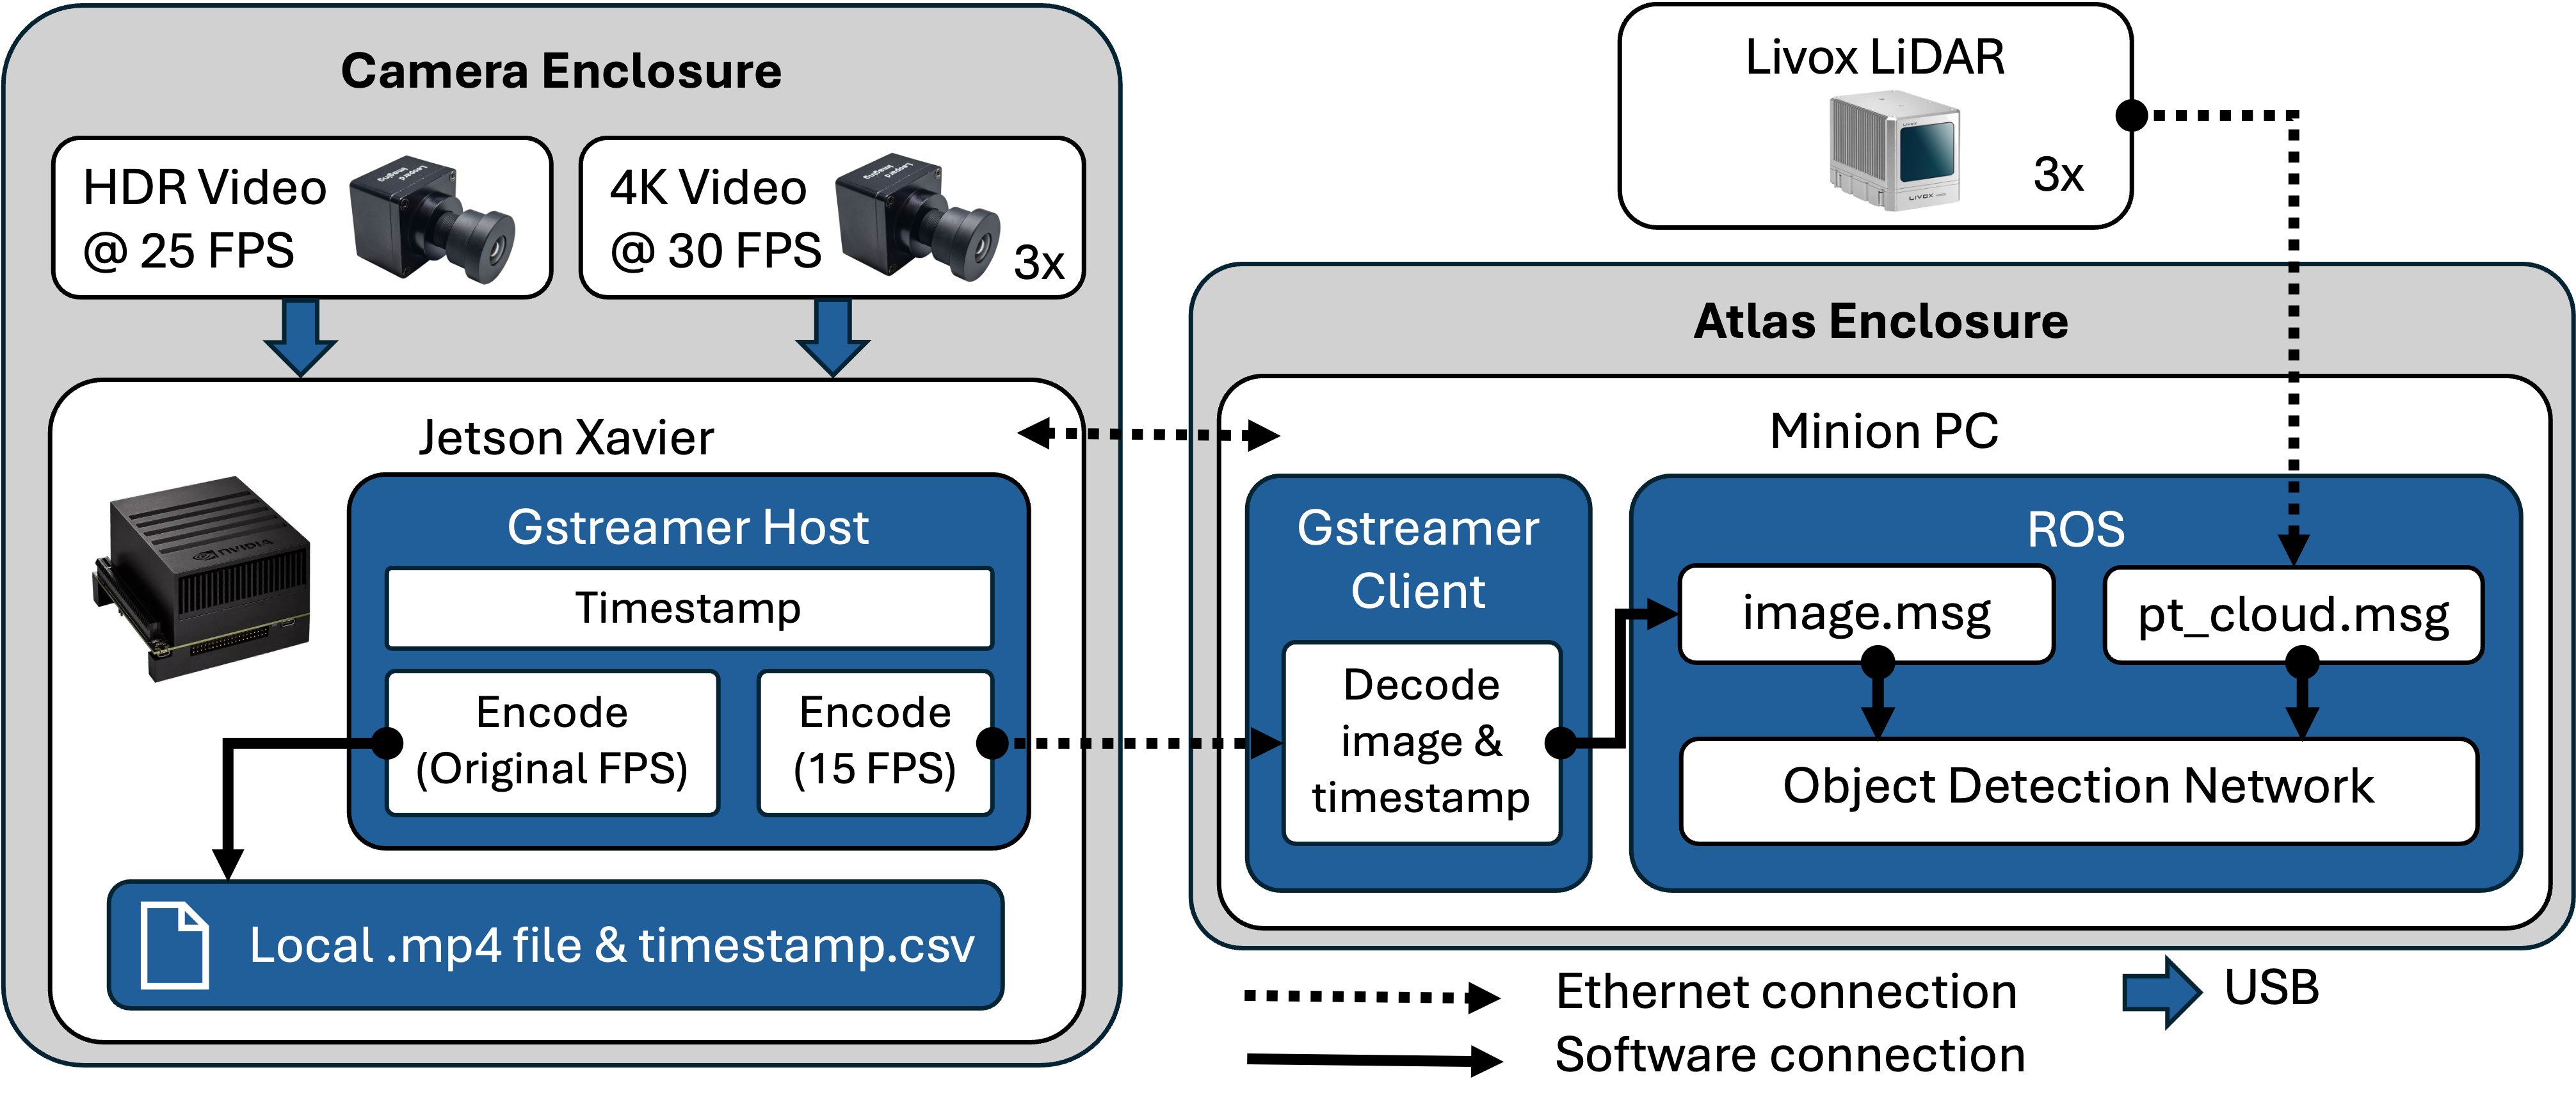
\includegraphics[width=5in]{Images/Video_Block_Diagram.png}
\caption{Block diagram of the vision system's hardware and video pipeline software.}
\label{video_pipeline}
\end{figure}



%%%%%%%%%%%%%%%%%%%%%%%%%%%%%%%%%%%%%%%%%%%%%%%%%%%%%%%%%%%%%%%%%%%%
%%%%%%%%%%%%%%%%%%%%%%%%%%%%%%%%%%%%%%%%%%%%%%%%%%%%%%%%%%%%%%%%%%%%
\section{Calibration Results} \label{sec:calib_results}

\subsection{Spatial Calibration}

% \begin{figure}[htbp]
%     \centering
%     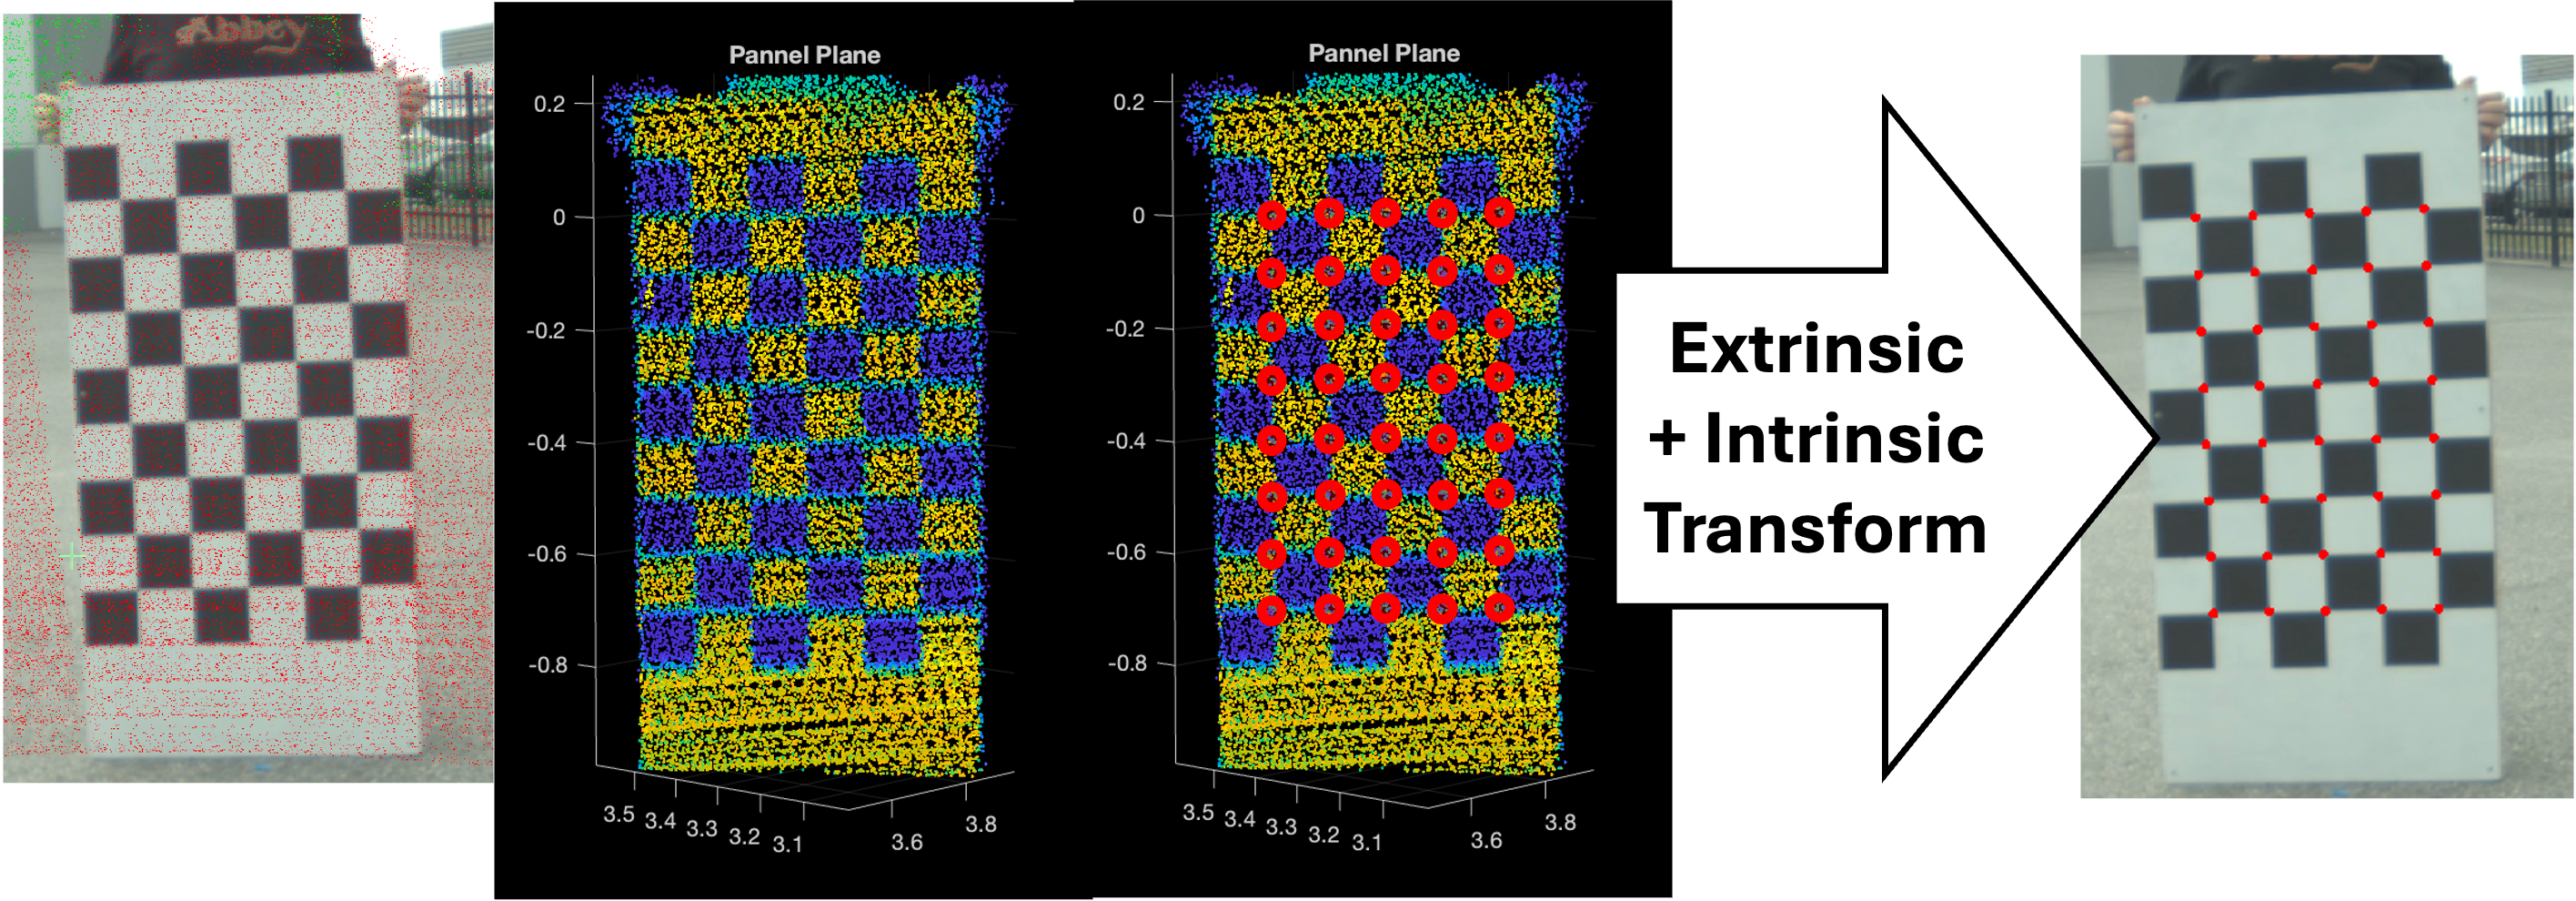
\includegraphics[width=0.8\linewidth]{Images/calib_checkers.png}
%     \caption{Caption}
%     \label{fig:calib_check}
% \end{figure}

% \begin{figure}[htbp]
%     \centering
%     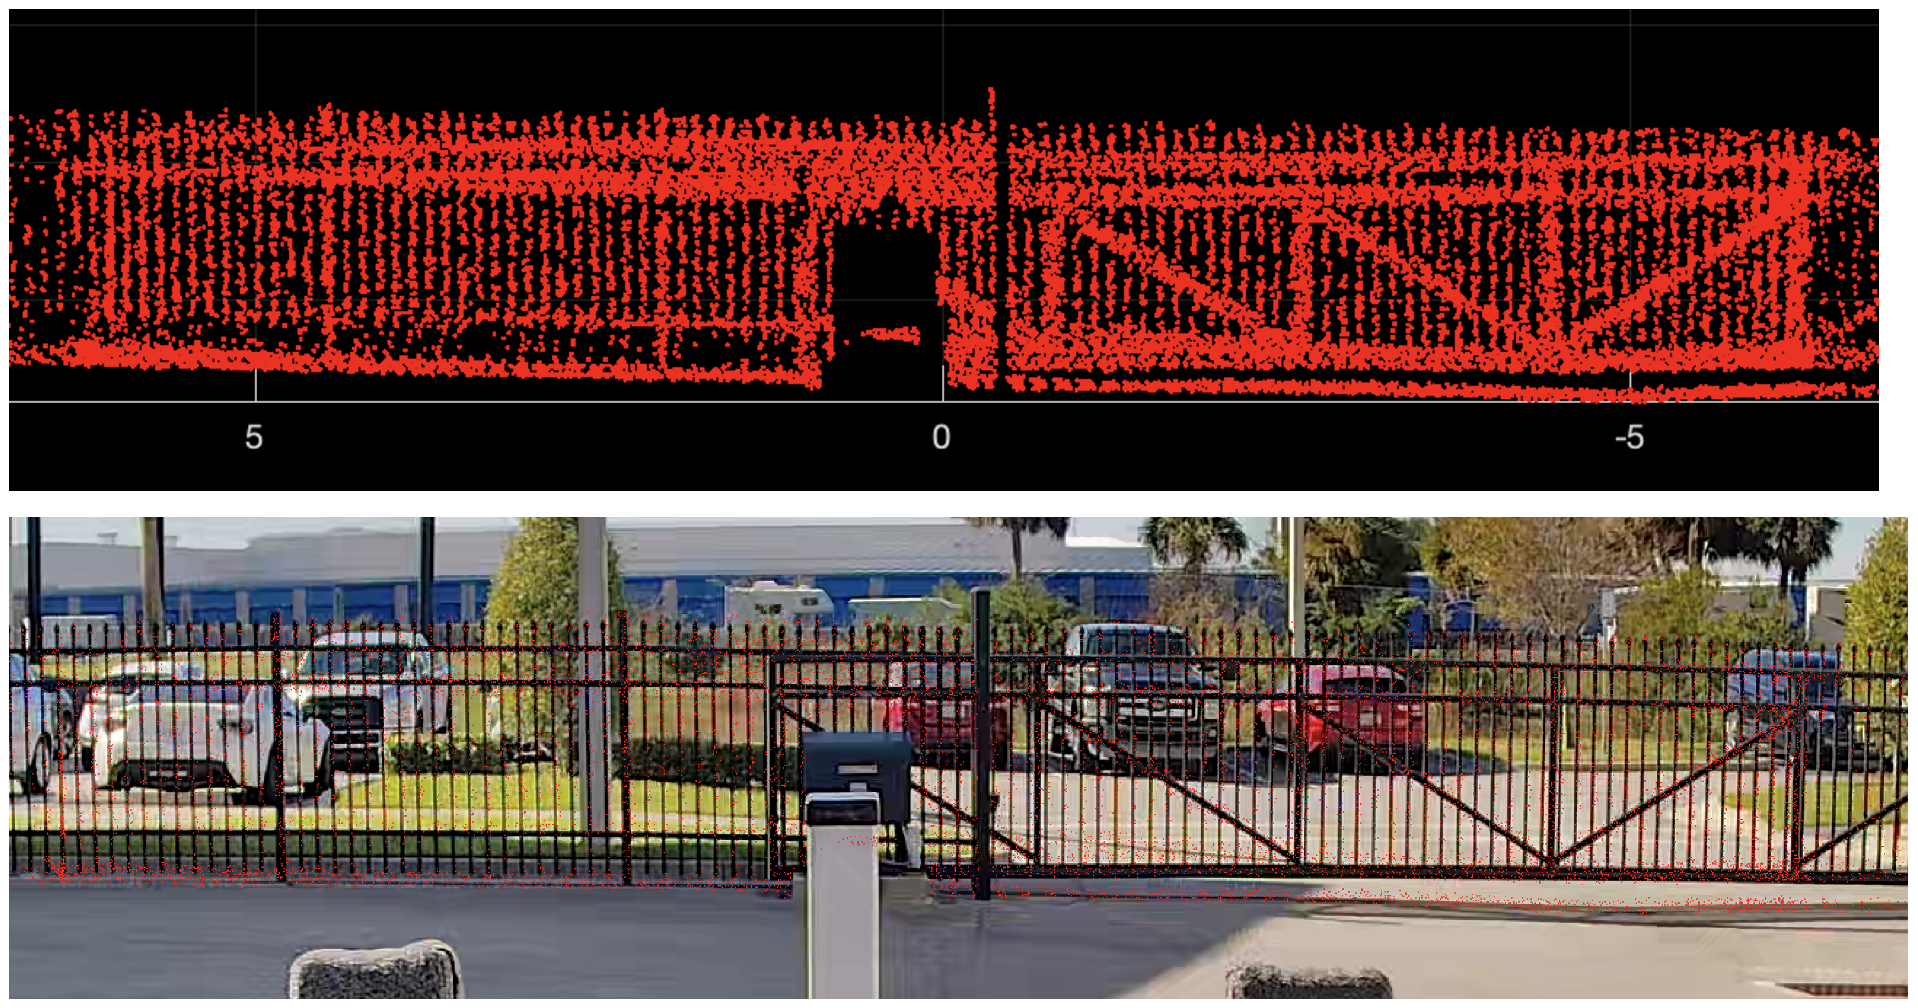
\includegraphics[width=0.8\linewidth]{Images/LiDAR_calib_fence.png}
%     \caption{Caption}
%     \label{fig:calib_fence}
% \end{figure}

\begin{figure}[htbp]
    \centering
    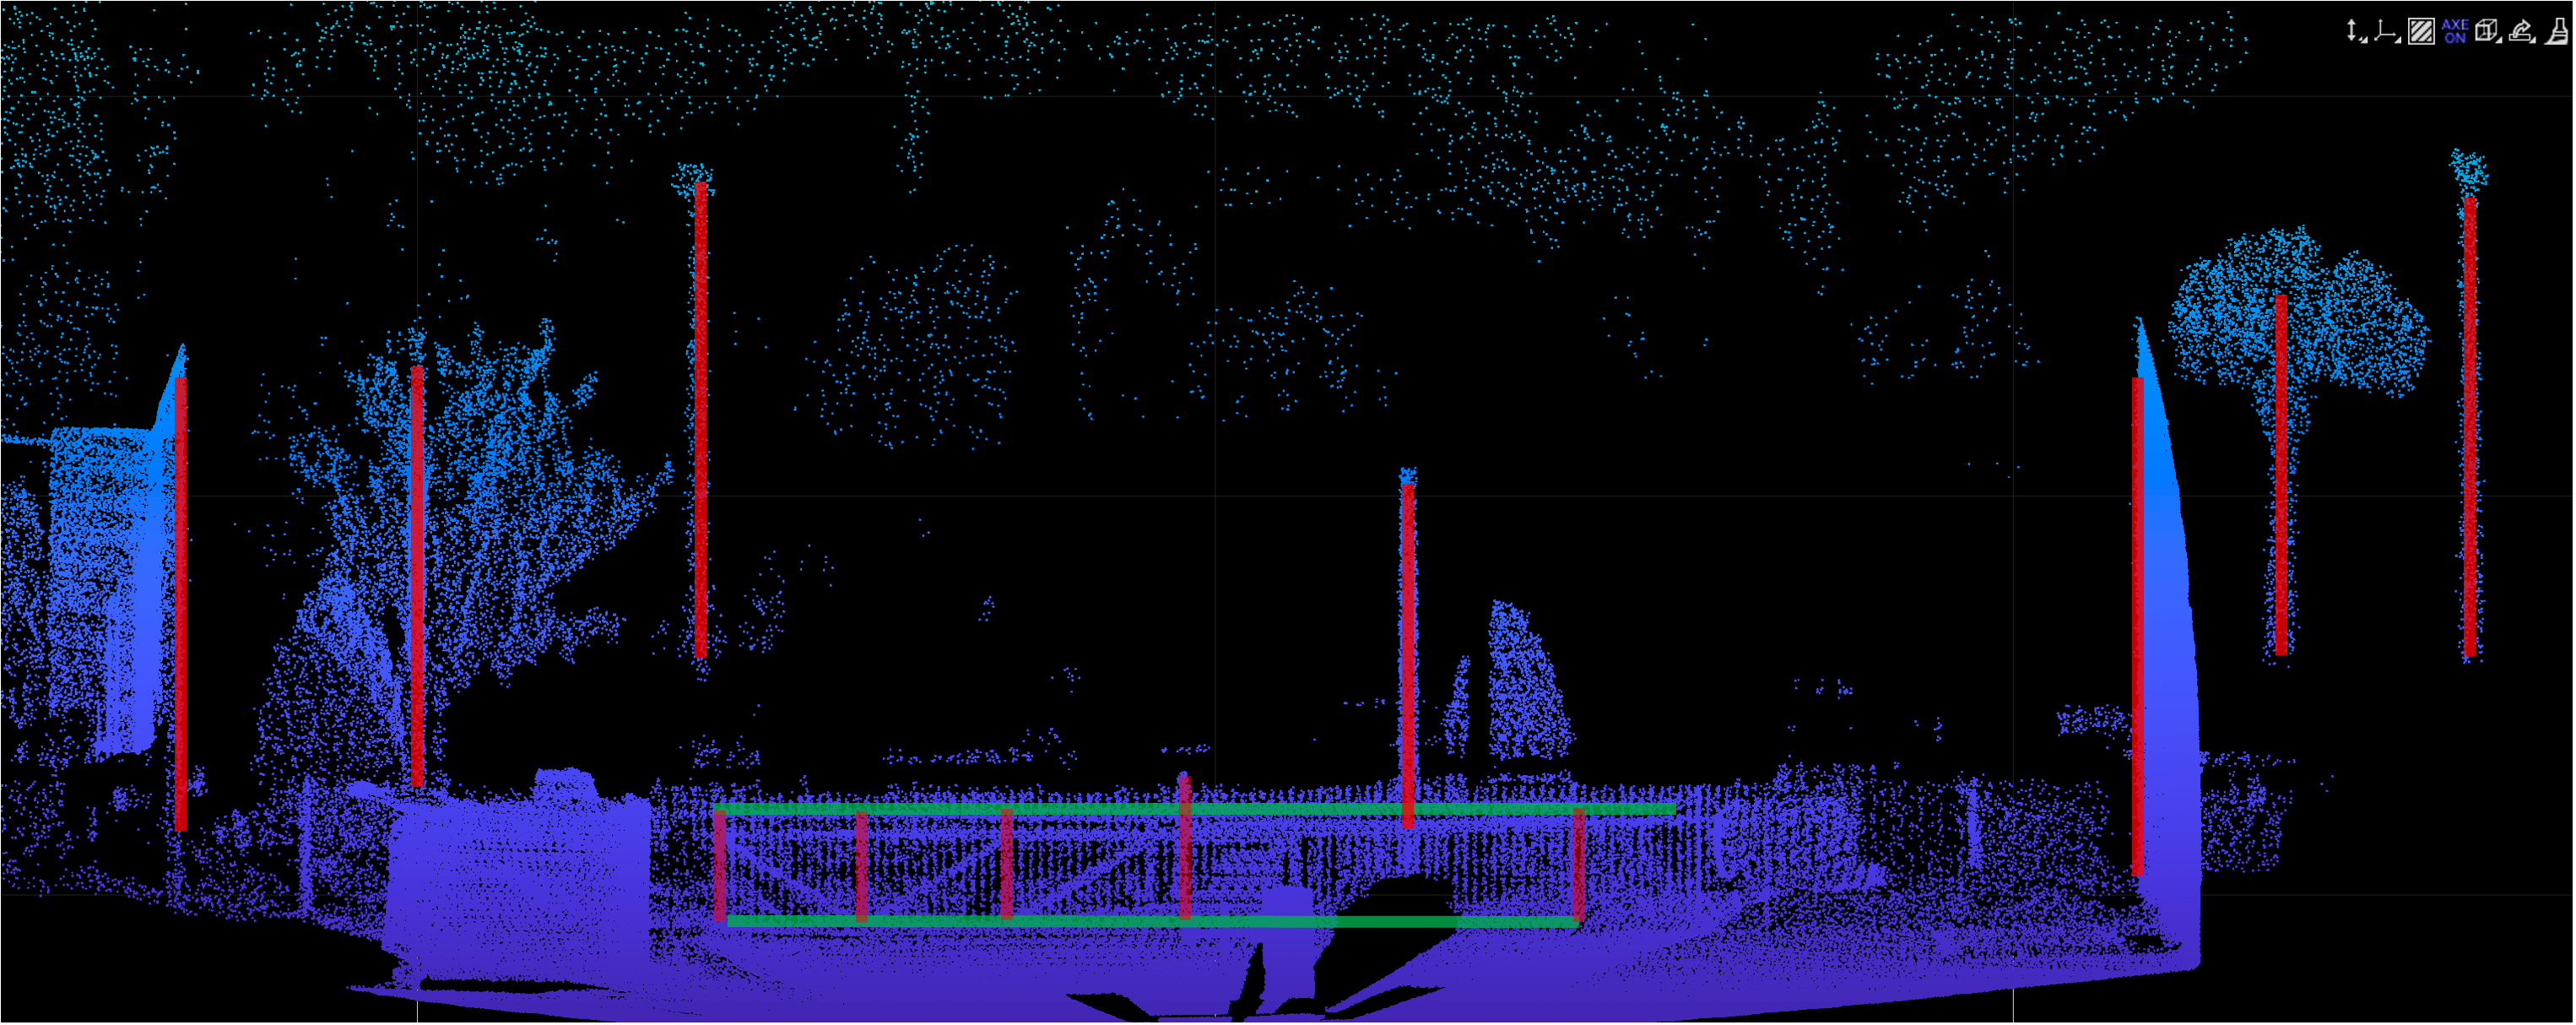
\includegraphics[width=0.8\linewidth]{Images/LiDAR_features.png}
    \caption{Caption}
    \label{fig:LiDAR_features}
\end{figure}


% \begin{figure}[htbp]
%     \centering
%     \includegraphics[width=0.8\linewidth]{Images/LiDAR_overlay.png}
%     \caption{Caption}
%     \label{fig:LiDAR_overlay}
% \end{figure}

% \begin{figure}[htbp]
%     \centering
%     \includegraphics[width=0.8\linewidth]{Images/LiDAR_overlay3A.png}
%     \caption{Caption}
%     \label{fig:LiDAR_overlay3A}
% \end{figure}

% \begin{figure}[htbp]
%     \centering
%     \includegraphics[width=0.8\linewidth]{Images/LiDAR_overlay3B.png}
%     \caption{Caption}
%     \label{fig:LiDAR_overlay3B}
% \end{figure}



% \begin{figure}[htbp]
%     \centering
%     \includegraphics[width=0.8\linewidth]{Images/LiDAR_overlay2.png}
%     \caption{Caption}
%     \label{fig:LiDAR_overlay2}
% \end{figure}

\begin{figure}[htbp]
    \centering
    \includegraphics[width=0.8\linewidth]{Images/LiDAR_overlay4.png}
    \caption{Caption}
    \label{fig:LiDAR_overlay4}
\end{figure}


\subsection{Temporal Calibration}

\begin{figure}[htbp]
    \centering
    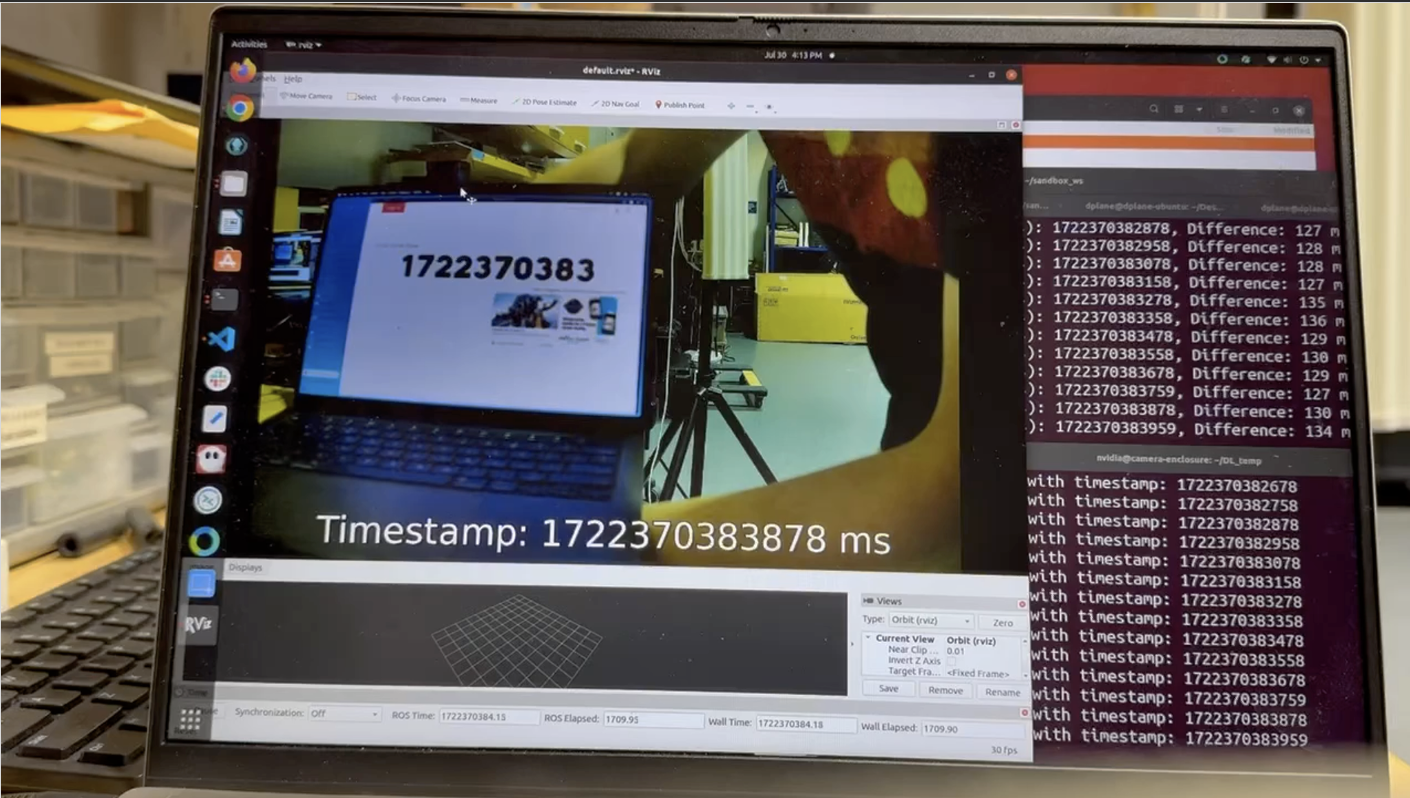
\includegraphics[width=0.8\linewidth]{Images/time_sync1.png}
    \caption{Caption}
    \label{fig:time_sync1}
\end{figure}

% ## Temporal Drift Analysis and Correction

Despite the hierarchical GPS-NTP-PTP synchronization architecture distributing a common time reference to all platform sensors, systematic timing offsets arise between video frames recorded locally on the NVIDIA Jetson Xavier camera enclosure and the same frames transmitted over the network and received as ROS messages on the Atlas PC.
These offsets originate from a combination of network latency, video encoding and decoding delays, frame buffering in the GStreamer pipeline, and potential residual clock drift between computing platforms.
Uncorrected timing discrepancies of 0.24 to 1.54 seconds compromise temporal alignment between camera observations and LiDAR point clouds.
For a vessel traveling at 5 meters per second, a 1-second timing error translates to 5 meters of spatial misalignment when attempting to associate camera frames with LiDAR observations, invalidating the frame-accurate sensor fusion required for rigorous detection performance analysis.

A comprehensive temporal drift analysis and correction methodology establishes ground-truth frame correspondence between locally-recorded video and network-transmitted ROS messages through structural similarity-based image matching, quantifies systematic timing offsets, characterizes drift patterns, and applies interpolation-based corrections to achieve sub-second temporal alignment accuracy.

% ### Problem Statement and Offset Sources

The distributed video processing architecture separates frame acquisition and encoding on the Jetson Xavier from reception and ROS publication on the Atlas PC.
This separation introduces timing discrepancies through multiple mechanisms.

Encoding and transmission delays arise as the H.264/H.265 encoding process introduces latency between frame capture and bitstream availability.
Network transmission adds additional delay, followed by RTP depacketization, parsing, and decoding on the receive side.
While the SEI timestamp embedded in each frame records the original capture time, the ROS message timestamp on the Atlas PC may differ due to buffering and processing delays.

Clock synchronization imperfections contribute to offsets.
Although both the Jetson Xavier and Atlas PC synchronize to GPS time via NTP, network latency and NTP algorithm behavior result in typical synchronization accuracy of 1-10 milliseconds.
Over extended recording sessions, differential clock drift between systems can accumulate, creating time-varying offsets.

Frame buffering in GStreamer's buffering mechanisms, designed to smooth network jitter and ensure continuous playback, introduces variable delays between frame availability and processing.
These delays manifest as offsets between the SEI-embedded acquisition timestamp and the ROS message publication time.

The cumulative effect produces systematic time offsets ranging from hundreds of milliseconds to multiple seconds between Jetson-recorded video timestamps and Atlas-received ROS message timestamps.

% ### Ground Truth Establishment via Image Matching

Quantifying temporal offsets requires establishing ground-truth correspondence between frames in locally-recorded video files and frames in ROS bag recordings.
This correspondence cannot be assumed based on frame count or relative timing, as dropped frames or transmission artifacts might desynchronize sequential indexing.
A content-based matching approach using the Structural Similarity Index Measure provides robust frame correspondence despite minor compression artifacts or brightness variations.

% #### Structural Similarity Index Measure

SSIM quantifies perceptual similarity between two images by comparing luminance, contrast, and structural patterns rather than simple pixel-wise differences.
The metric ranges from 0.0 indicating completely dissimilar images to 1.0 indicating identical images, with values above 0.6-0.7 typically indicating the same scene despite minor variations in encoding, brightness, or noise.

For two image patches $x$ and $y$, SSIM is computed as:

\begin{equation}
    \text{SSIM}(x,y) = \frac{(2\mu_x\mu_y + C_1)(2\sigma_{xy} + C_2)}{(\mu_x^2 + \mu_y^2 + C_1)(\sigma_x^2 + \sigma_y^2 + C_2)}
\end{equation}


where $\mu$ denotes mean luminance, $\sigma^2$ denotes variance, $\sigma_{xy}$ denotes covariance, and $C_1$, $C_2$ are stabilization constants.

SSIM proves superior to mean squared error or peak signal-to-noise ratio for this application because it tolerates the slight brightness and contrast variations introduced by independent H.264/H.265 encoding of the same source frames on the Jetson for local recording versus the Atlas after ROS decoding.

% #### Frame Matching Implementation

A custom Python analysis tool was developed to extract frames from both locally-saved video files and ROS bag recordings, then perform SSIM-based matching.

Video frame extraction uses OpenCV to read all frames with timestamps from MP4 or MKV video files, computing relative timestamps based on frame number and video frame rate.

ROS bag frame extraction reads image messages from ROS bag files, extracting ROS timestamps from message headers and converting ROS image messages to OpenCV format using the cv\_bridge library.

SSIM computation converts images to grayscale for computational efficiency, resizes images if dimensions differ, and computes the structural similarity score using implementations from scikit-image.

% ### Hybrid Manual-Automated Matching Strategy

The frame matching procedure employs a hybrid approach where initial synchronization points are established through intensive brute-force SSIM comparison, then subsequent matches leverage the learned time offset for computational efficiency.

% #### Phase 1: Initial Synchronization Points

For each ROS bag file, the first 5 message frames undergo exhaustive SSIM matching against a search window in the corresponding video file.

The search window spans ±15 seconds, equivalent to 375 frames at 25 fps, sufficient to accommodate potential multi-second timing offsets while remaining computationally tractable.
For each ROS frame, SSIM scores are computed between the ROS frame and all video frames in the search window.
The video frame with the highest SSIM score is selected as the best match, provided the score exceeds the 0.6 threshold indicating acceptable match quality.

% #### Phase 2: Offset Validation

Once initial synchronization points are established, time offsets are computed as the difference between video timestamp and ROS timestamp.
Offset consistency is verified across sync points.

If the standard deviation of offsets across the first 5 sync points exceeds 0.1 seconds, the methodology flags the bag-video pair for manual review, as large offset variability suggests non-linear drift or frame matching errors.

% #### Phase 3: Automated Processing

For ROS messages beyond the initial 5 manual sync points, the learned average offset enables efficient matching.
The ROS timestamp is adjusted by the learned offset to compute the expected video frame number, reducing computational cost from order $n \times m$ for exhaustive SSIM comparison to order $n$ for timestamp-based lookup, where $n$ is the number of ROS messages and $m$ is the search window size.

% ### Database Implementation for Scalability

The temporal drift analysis processes 107,968 total ROS image messages across multiple recording sessions.
A SQLite database provides structured storage for synchronization points, offsets, and validation metrics.

The database schema includes tables linking bag files to video files and recording frame synchronization points including ROS timestamps, video timestamps, video frame numbers, time offsets, SSIM scores, and estimation quality classification distinguishing exact matches from interpolated and extrapolated values.

The database enables queries for drift analysis calculating offset changes and drift rates over time, supporting temporal alignment validation across the complete dataset.

% ### Temporal Drift Characteristics

Analysis of the synchronization database reveals systematic patterns in timing offsets.

% #### Offset Magnitude and Stability

Typical offset ranges span 0.24 to 1.54 seconds across different bag-video pairs.
Offset standard deviations range from 0.01 to 0.08 seconds within individual recording sessions.
Drift rates range from -0.17 to +0.01 seconds per second.

Negative drift rates indicate that ROS message timestamps advance faster than video timestamps, equivalently that the time offset decreases over the session, suggesting slight residual clock drift between Jetson Xavier and Atlas PC despite NTP synchronization.

% #### Network Jitter Contribution

The ±0.081 second standard deviation observed in some sessions indicates network-induced timing variability.
UDP transport used for RTSP streaming offers no delivery guarantees, and occasional network jitter manifests as frame arrival time variations that GStreamer buffering mechanisms smooth but do not eliminate entirely.

% #### Systematic Offset Sources

The consistent 0.24-1.54 second offset magnitude exceeds the expected NTP synchronization error of 1-10 milliseconds by orders of magnitude, indicating that the primary offset source is not clock drift but rather pipeline latency.
The video encoding, transmission, and decoding chain introduces delays accumulating to hundreds of milliseconds or seconds, necessitating correction beyond simple clock synchronization to achieve frame-accurate temporal alignment.

% ### Interpolation-Based Timestamp Correction

Establishing synchronization points approximately every 1 second, equivalent to 10 ROS messages at 10 Hz sampling rate, enables accurate interpolation of corrected timestamps for all frames including those between explicit sync points.

% #### Linear Interpolation Method

Using SciPy's interpolation functions, mapping functions are created from ROS timestamps to video frame numbers based on established synchronization points.
For any ROS message with timestamp falling between two synchronization points, the corresponding video frame number is estimated through linear interpolation.

The linear interpolation assumption holds well given observed drift characteristics where drift rates typically remain below ±0.2 seconds per second, producing nearly linear offset evolution between 1-second sync points.

% #### Validation Metrics

Interpolation accuracy is validated by comparing predicted frame numbers against ground-truth SSIM matches.

Mean absolute error remains under 1 frame, equivalent to under 40 milliseconds at 25 fps.
Root mean square error remains under 2 frames, representing under 80 milliseconds.
Maximum errors of 3-5 frames represent under 200 milliseconds.

These accuracy levels achieve sub-second temporal alignment meeting requirements for associating camera frames with LiDAR observations for object detection evaluation.

% #### Quality Classification

Each timestamp correction is classified by estimation quality.

Exact match designates cases where the ROS timestamp exactly matches a synchronization point with SSIM greater than 0.6.
Interpolated designates cases where linear interpolation occurs between two synchronization points.
Extrapolated designates cases outside the range of synchronization points, indicating lower confidence.

% ### Corrected Dataset Generation

The drift correction methodology produces a comprehensive temporal alignment dataset for each bag-video pair.

For each ROS frame, the corresponding video frame is estimated using the interpolation function.
The corrected timestamp is computed from the estimated frame number and video frame rate.
The applied time offset is calculated as the difference between estimated video timestamp and original ROS timestamp.
Estimation quality is determined based on whether the ROS timestamp matches a sync point, falls between sync points, or lies outside the sync point range.

Output CSV files provide corrected timestamps for all frames in each recording session, enabling downstream sensor fusion pipelines to apply accurate temporal alignment.

The dataset contains 10,141 exact matches representing 9.4% of total frames, 96,827 interpolated frames representing 89.7%, and 1,000 extrapolated frames representing 0.9%.
The high interpolation fraction reflects the computational efficiency optimization that establishes explicit sync points for only a subset of frames while interpolating the remainder.

% ### Integration with Sensor Fusion Pipeline

The temporal drift correction methodology directly enables multi-modal sensor fusion by ensuring camera frame timestamps accurately reflect acquisition time.

Before correction, camera-LiDAR temporal alignment errors of 0.24-1.54 seconds produce spatial misalignment of 1.2-7.7 meters at 5 meters per second vessel speed, invalid temporal correlation between modalities, and potential false negative detections due to temporal mismatch.

After correction, camera-LiDAR temporal alignment improves to under 0.1 second typical interpolation error, spatial misalignment reduces to under 0.5 meters at 5 meters per second vessel speed, valid frame-accurate temporal association is established, and reliable cross-modal detection comparison becomes possible.

% ### Methodology Validation

Several validation procedures confirm the accuracy of the temporal drift correction.

% #### SSIM Score Distribution

The distribution of SSIM scores for matched frames indicates match quality.
Mean SSIM reaches 0.72, median SSIM reaches 0.73, the 95th percentile exceeds 0.85, and matches with SSIM below 0.6 representing less than 2 percent are flagged for manual review.
The high SSIM scores confirm reliable frame matching despite independent encoding paths.

% #### Offset Consistency

For recording sessions with stable operation, time offsets exhibit standard deviation under 0.05 seconds over 60-second periods, confirming the linear drift assumption.

% #### Monotonicity

Corrected timestamps maintain strict monotonic increase, confirming no frame reordering or duplicate frame issues.

% #### Visual Inspection

Random sampling of matched frames for visual comparison by human observers confirms that SSIM matches correspond to identical scene content.

% ### Limitations and Assumptions

The temporal drift analysis methodology assumes several conditions.

Linear drift between sync points is approximately valid for 1-second intervals but may degrade for longer periods.
SSIM reliability requires sufficient visual features; feature-sparse maritime scenes including open water or fog may reduce match confidence.
No dropped frames are assumed; the methodology assumes all captured frames reach the ROS bag, as dropped frames would require more sophisticated matching.
Constant frame rate is assumed; variable frame rate would complicate interpolation.

Despite these limitations, the methodology achieves the sub-second temporal alignment necessary for rigorous object detection performance comparison between sensing modalities.




%%%%%%%%%%%%%%%%%%%%%%%%%%%%%%%%%%%%%%%%%%%%%%%%%%%%%%%%%%%%%%%%%%%%
%%%%%%%%%%%%%%%%%%%%%%%%%%%%%%%%%%%%%%%%%%%%%%%%%%%%%%%%%%%%%%%%%%%%
% \section{Sensor Data} \label{sensor_data}

% ROS
%    - image of ROS node structure from RobotX paper
% table of msgs & rates within each bagfile

%%%% From atlas %%%
% The ROS ecosystem provides integrated data recording functionality through the `rosbag` utility (ROS 1) and `ros2 bag` (ROS 2), which subscribe to specified ROS topics and serialize all messages to disk in a format that enables precise temporal replay. The Atlas platforms employ this infrastructure to record sensor data during data collection operations, capturing synchronized streams of:

% - Raw LiDAR point clouds from all three Livox sensors
% - Compressed video streams with embedded timestamps from all three cameras
% - GPS/INS pose estimates with timestamp and uncertainty information
% - Detection results from vision and LiDAR object detection algorithms
% - Platform status messages, network diagnostics, and operator annotations

% The resulting bag files serve as the ground-truth dataset for the detection performance analysis presented in Chapter 6, with temporal drift correction procedures detailed in [[03_Temporal_Drift|Section 3.2.2.3]] ensuring frame-accurate alignment between modalities within the recorded data.

%%%%%%%%%%%%%%%%%%%%%%%%%%%%%%%%%%%%%%%%%%%%%%%%%%%%%%%%%%%%%%%%%%%%
%%%%%%%%%%%%%%%%%%%%%%%%%%%%%%%%%%%%%%%%%%%%%%%%%%%%%%%%%%%%%%%%%%%%
%%%%%%%%%%%%%%%%%%%%%%%%%%%%%%%%%%%%%%%%%%%%%%%%%%%%%%%%%%%%%%%%%%%%
\chapter{Sensor Data and Dataset} \label{dataset}

\section{ROS Architecture} \label{ROS_architechture}

\subsection{ROS Messages} \label{ROS_mesages}

\begin{table}[htbp]
\centering
\begin{tabular}{lcc}
\hline
ROS Topic & Typical Bandwidth (Mbps) & \% Total Bandwidth \\
\hline
/points\_livox\_front & 35--40 & 3.5--4.0 \\
/points\_livox\_port  & 35--40 & 3.5--4.0 \\
/points\_livox\_starboard & 35--40 & 3.5--4.0 \\
/image\_hdr\_raw  & 60--70 & 6.0--7.0 \\
\hline
\textbf{Total Estimated Utilization} & \textbf{165--190} & \textbf{17--19 \%} \\
\hline
\end{tabular}
\label{table:ROS_bandwidth}
\caption{Approximate \ac{ROS} message bandwidth utilization for the topics used in this research, relative to a 1 Gbps Ethernet link ($\sim$940 Mbps usable).}
\end{table}

\section{ROS Bags} \label{ROS_bags}

The \ac{ROS} ecosystem provides integrated data recording utilities that subscribe to designated topics and serialize all messages to disk for precise temporal replay.
The Atlas systems employ this infrastructure to record synchronized streams of sensor and perception data, including:

\begin{itemize}
\item Raw point clouds from all three Livox Horizon \ac{LiDAR} sensors
\item Compressed video streams with embedded timestamps from each camera
\item GPS/INS pose estimates with timestamp and uncertainty data
\item Detection outputs from vision and \ac{LiDAR}-based object detection algorithms
\item Platform status, network diagnostics, and operator annotations
\end{itemize}

The resulting bag files serve as the ground-truth datasets for detection performance analysis (see Chapter~\ref{dataset}).
Temporal synchronization procedures described in Section~\ref{time_sync} ensure frame-accurate alignment across all modalities within these recordings.

The storage subsystem sustains aggregate write rates exceeding 200 MBps during full-sensor operation.
Measured JPEG images extracted from the recorded ROS bags averaged approximately 0.5~MB per frame.
At the 5 fps capture rate used during training datasets, this corresponds to about 2.5 MBps per camera, while the 15 fps rate used during RobotX competition runs produced roughly 7.5 MBps per camera. 
Including ROS message encapsulation and metadata, total write rates during full-sensor operation typically ranged from 60 to 100 MBps when accounting for LiDAR, GPS/INS, and detection topics. 
These rates remain well within the sustained throughput capability of the NVMe solid-state drives, enabling extended recording sessions without frame loss or buffer overflow.

Post-processing workflows access these bag files to extract synchronized observations for offline analysis.
The preserved timestamps enable sub-millisecond temporal alignment between locally recorded frames on the Jetson Xavier and those received via RTSP and stored on the Atlas PCs—an essential capability for the multi-modal performance comparisons presented in Chapters~\ref{dataset}–\ref{realtime_object_detection}.



%%%%%%%%%%%%%%%%%%%%%%%%%%%%%%%%%%%%%%%%%%%%%%%%%%%%%%%%%%%%%%%%%%%%
%%%%%%%%%%%%%%%%%%%%%%%%%%%%%%%%%%%%%%%%%%%%%%%%%%%%%%%%%%%%%%%%%%%%
%%%%%%%%%%%%%%%%%%%%%%%%%%%%%%%%%%%%%%%%%%%%%%%%%%%%%%%%%%%%%%%%%%%%
\chapter{Real-time Object Detection} \label{realtime_object_detection}


%%%%%%%%%%%%%%%%%%%%%%%%%%%%%%%%%%%%%%%%%%%%%%%%%%%%%%%%%%%%%%%%%%%%
%%%%%%%%%%%%%%%%%%%%%%%%%%%%%%%%%%%%%%%%%%%%%%%%%%%%%%%%%%%%%%%%%%%%
\section{YOLOv8} \label{yolo}

Camera-based perception provides rich visual information about the maritime environment, capturing texture, color, and fine geometric detail that can distinguish object types through learned visual features.
For real-time autonomous navigation, the detection system must process high-resolution imagery at frame rates sufficient to maintain situational awareness while an \ac{USV} maneuvers through dynamic environments.
\textcolor{red}{I employed the YOLOv8 architecture from Ultralytics for vision-based maritime object detection due to its demonstrated balance between detection accuracy and computational efficiency in real-time applications.}

%%%%%%%%%%%%%%%%%%%%%%%%%%%%%%%%%%%%%%%%%%%%%%%%%%%%%%%%%%%%%%%%%%%%
\subsection{YOLO Architecture } \label{sec:yolo_architecture}

YOLO (You Only Look Once) represents a family of single-stage object detection architectures that frame detection as a regression problem rather than a classification task applied to region proposals.
The architecture processes an entire image in a single forward pass through a convolutional neural network, directly predicting bounding boxes and class probabilities for objects present in the scene.
This single-stage approach enables real-time performance by eliminating the computational overhead of region proposal generation and iterative refinement stages required by two-stage detectors such as R-CNN variants \cite{ultralytics}.

YOLOv8, released by Ultralytics in 2023, incorporates several architectural improvements over previous YOLO versions that enhance detection performance for small objects and complex scenes.
The backbone network employs a CSPDarknet architecture with cross-stage partial connections that enable efficient gradient flow during training while maintaining representational capacity.
The neck utilizes a Path Aggregation Network (PANet) structure to fuse features across multiple scales, allowing the detector to leverage both high-resolution spatial information from early layers and semantic information from deeper layers.
The detection head employs an anchor-free approach with decoupled classification and localization branches, simplifying the training process and improving generalization to objects with varying aspect ratios.

For maritime object detection, the standard YOLOv8 architecture requires minimal domain-specific modifications because the model's design already accommodates multi-scale detection across a range of object sizes.
Maritime objects such as navigation buoys span scales from small distant targets occupying tens of pixels to large nearby vessels filling substantial portions of the image frame.
The YOLOv8 architecture's three-scale detection strategy with stride values of 8, 16, and 32 pixels naturally aligns with this scale distribution, enabling detection of buoys at distances exceeding 50 meters alongside larger vessels at closer range.

The primary adaptation for maritime deployment involves training the model on domain-specific data representing the visual characteristics of the target environment.
Maritime scenes differ substantially from the general-purpose datasets such as COCO (Common Objects in Context) used for pre-training foundational computer vision models.
Water surfaces introduce specular reflections, variable lighting conditions from sun glare, and wave motion that creates dynamic occlusion patterns not present in terrestrial imagery.
Objects appear against relatively uniform backgrounds with fewer contextual cues compared to urban or indoor scenes where surrounding objects provide spatial relationships that aid detection.
Training on maritime-specific data enables the model to learn visual features robust to these environmental characteristics while leveraging transfer learning from pre-trained weights to reduce training time and data requirements.

%%%%%%%%%%%%%%%%%%%%%%%%%%%%%%%%%%%%%%%%%%%%%%%%%%%%%%%%%%%%%%%%%%%%
\subsection{Model Selection} \label{sec:yolo_model_selection}

The YOLOv8 family includes five model variants (n, s, m, l, x) spanning a range of network depths and widths that trade detection accuracy for computational efficiency.
I selected the YOLOv8-small (YOLOv8s) variant for deployment on the Minion platform based on hardware constraints and real-time performance requirements.
The YOLOv8s model contains 11.2 million parameters and achieves competitive accuracy on benchmark datasets while maintaining inference speeds suitable for real-time operation on GPU-accelerated hardware.

Smaller variants such as YOLOv8-nano (YOLOv8n) offer faster inference at the expense of detection accuracy, particularly for small or distant objects where reduced network capacity limits the model's ability to learn discriminative features.
Larger variants (YOLOv8-medium through YOLOv8-extra-large) improve accuracy through increased representational capacity but require proportionally more computational resources, potentially preventing real-time operation on the embedded computing platform.
The YOLOv8s variant provides an effective balance for maritime object detection where small buoys at medium to long range represent the most challenging detection targets.

Implementation employed the Ultralytics Python library, which provides a unified interface for training, validation, and deployment of YOLOv8 models.
The framework handles data loading, augmentation, training loop management, and model export, allowing focus on maritime-specific considerations such as dataset preparation and hyperparameter tuning.
The library supports export to multiple inference formats including PyTorch, ONNX, and TensorRT, enabling deployment flexibility across different hardware platforms and optimization backends.

For the Minion platform, I configured the model for inference at the native resolution of the Leopard Imaging IMX490 \ac{HDR} camera (2880×1860 pixels).
Processing full-resolution imagery preserves fine spatial detail necessary for detecting small distant buoys while avoiding information loss from aggressive downsampling.
The model input preprocessing pipeline applies standard normalization to [0,1] range and organizes image data in RGB channel order following PyTorch conventions.
No additional image preprocessing such as histogram equalization or contrast enhancement is performed during inference, as the model learns to handle the natural dynamic range variations present in \ac{HDR} imagery during training.

%%%%%%%%%%%%%%%%%%%%%%%%%%%%%%%%%%%%%%%%%%%%%%%%%%%%%%%%%%%%%%%%%%%%
\subsection{Training Data} \label{sec:yolo_training data}

The training dataset consists of annotated video frames extracted from ROS bag files recorded during the 2024 Maritime RobotX Challenge and associated training missions.
Frame extraction occurs at 1 Hz to provide temporal diversity while avoiding excessive correlation between consecutive frames that would artificially inflate apparent dataset size without corresponding information gain.
The resulting dataset contains several thousand annotated images spanning diverse maritime conditions including varying lighting (morning, midday, afternoon), weather (clear, overcast, light rain), and sea states (calm to moderate chop).

Ground truth annotations follow the COCO format with bounding boxes specified as $[x, y, width, height]$ in pixel coordinates along with corresponding class labels.
I annotated six object classes relevant to autonomous maritime navigation: tall cylindrical buoys (tall\_buoy), spherical navigation markers (round\_buoy encompassing both A2 and A3 buoy types), light towers (light\_tower), recreational vessels (jon\_boat), and sailboats (sailboat).
The round\_buoy class combines A2 and A3 buoys into a single category because visual distinction between these buoy types proves challenging even for human annotators when objects appear at medium to long range where geometric details become ambiguous.

Annotation quality directly impacts detection performance, particularly for small objects where even single-pixel boundary errors represent significant proportional inaccuracies.
I employed a hybrid manual-automated annotation approach where an initial trained model generated candidate bounding boxes that were manually reviewed and corrected.
This approach improves annotation efficiency while maintaining quality through human verification of all final annotations.
Annotations include only fully visible objects with sufficient resolution for class identification; partially occluded or extremely distant objects below reliable identification threshold are excluded from ground truth to avoid introducing label noise.

The dataset exhibits class imbalance reflecting the natural distribution of object encounters during data collection missions.
Tall buoys appear most frequently due to their use as primary navigation markers in the competition course, while sailboats and light towers appear less frequently as they represent environmental background objects rather than task-specific targets.
Training procedures account for this imbalance through class-weighted loss functions that prevent the model from learning a trivial classifier biased toward majority classes.

Data augmentation techniques adapt standard computer vision augmentation strategies to maritime-specific considerations.
Geometric augmentations include random horizontal flips (maritime scenes exhibit left-right symmetry), random scaling (simulating varying object distances), and random perspective transforms (simulating different viewing angles).
Photometric augmentations include brightness and contrast adjustments (representing natural lighting variations), hue-saturation modifications (accounting for water color changes under different sky conditions), and simulated motion blur (representing relative motion between platform and objects in rough seas).
Augmentations are applied probabilistically during training with intensity bounds calibrated to remain within plausible maritime scene parameters, avoiding unrealistic transformations that could degrade rather than enhance model robustness.

%%%%%%%%%%%%%%%%%%%%%%%%%%%%%%%%%%%%%%%%%%%%%%%%%%%%%%%%%%%%%%%%%%%%
\subsection{Model Training and Convergence} \label{sec:yolo_training convrg}

Model training employed transfer learning from YOLOv8s weights pre-trained on the COCO dataset.
Pre-training provides initialization with general object detection capabilities including edge detection, shape recognition, and multi-scale feature extraction that accelerate convergence on the maritime-specific detection task.
The final detection head layer was reinitialized to accommodate the six maritime object classes, as COCO's 80 classes do not include maritime navigation markers.

Training utilized the AdamW optimizer with an initial learning rate of 0.001 and cosine annealing schedule that gradually reduces the learning rate to 0.0001 over the training duration.
Weight decay was set to 0.0005 to provide mild regularization preventing overfitting on the relatively small maritime dataset compared to large-scale general object detection benchmarks.
Batch size was configured at 16 images per iteration, representing the maximum size supportable on available GPU memory (24 GB on NVIDIA RTX 3090) while processing full-resolution imagery.

The training objective combines classification loss (binary cross-entropy), localization loss (complete IoU), and objectness loss (binary cross-entropy) with weighting factors that balance contributions from each component.
Classification loss penalizes incorrect class predictions, localization loss penalizes bounding box position and size errors, and objectness loss penalizes the confidence prediction for presence or absence of objects.
The complete IoU (CIoU) formulation for localization loss incorporates overlap ratio, center point distance, and aspect ratio difference, providing more informative gradients than standard IoU loss particularly for small objects where traditional IoU can be unstable.

Training proceeded for 100 epochs with validation performed every 5 epochs on a held-out validation set comprising 20% of annotated frames.
Convergence typically occurred within 50-70 epochs as indicated by validation loss plateauing and validation mAP (mean Average Precision) stabilizing.
Early stopping with patience of 20 epochs prevented unnecessary training once validation metrics ceased improving, avoiding overfitting that can occur with extended training on limited datasets.

The trained model achieved competitive detection performance on the maritime validation set with mAP@0.5 (mean Average Precision at IoU threshold 0.5) exceeding 0.75 for most object classes.
Performance varied by class with tall buoys achieving highest precision due to their distinctive cylindrical shape and frequent appearance in training data, while sailboats exhibited lower precision reflecting their visual similarity to other vessel types and less frequent training examples.
Small distant objects presented greater detection challenges than large nearby objects, as expected given the reduced pixel area and limited visual features available at long range.

%%%%%%%%%%%%%%%%%%%%%%%%%%%%%%%%%%%%%%%%%%%%%%%%%%%%%%%%%%%%%%%%%%%%
\subsection{Computational Efficiency} \label{sec:yolo_efficiency}

Inference performance on the Minion platform was evaluated using ROS bag playback at real-time rate to simulate operational conditions.
The YOLOv8s model processing 2880×1860 pixel images achieved inference speeds of approximately 40-50 milliseconds per frame on the NVIDIA RTX 3090 GPU, corresponding to 20-25 \ac{fps} throughput.
This performance comfortably exceeds the 10 \ac{fps} camera frame rate employed during data collection, enabling real-time detection with computational headroom for additional perception processing tasks.

Inference time breakdown reveals that the forward pass through the neural network consumes the majority of processing time (35-40 ms), with post-processing including non-maximum suppression (NMS) and bounding box decoding requiring the remaining 5-10 ms.
NMS filters duplicate detections of the same object by suppressing lower-confidence boxes that substantially overlap higher-confidence detections for the same class.
The NMS IoU threshold was set to 0.45, meaning boxes with overlap exceeding 45% are considered duplicate detections of the same object.

Computational resource utilization during inference remained modest with GPU memory consumption around 4 GB including model weights, activation maps, and batch processing buffers.
This memory footprint represents less than 20% of available GPU memory on the RTX 3090, leaving substantial capacity for potential model scaling or concurrent processing tasks.
CPU utilization remained low (under 10% on the Intel i7 processor) as image decoding and data movement between CPU and GPU memory represent minor components of the inference pipeline compared to GPU-accelerated neural network computation.

The model demonstrates stable performance across varying environmental conditions encountered in maritime operations.
Detection accuracy remains consistent across different times of day with minimal degradation under morning/evening lighting compared to midday sun, indicating that training data augmentation successfully imparted robustness to illumination variations.
Moderate sea states with wave motion and vessel roll do not significantly impact detection rates for objects maintaining sufficient visibility, though extreme conditions with heavy spray or severe vessel motion can introduce motion blur that degrades detection of small distant targets.

%%%%%%%%%%%%%%%%%%%%%%%%%%%%%%%%%%%%%%%%%%%%%%%%%%%%%%%%%%%%%%%%%%%%
\subsection{Limitations} \label{sec:yolo_limitations}

Vision-based detection with YOLOv8 exhibits several limitations inherent to camera-based perception in maritime environments.
Adverse weather conditions including fog, heavy rain, and sea spray degrade image quality and consequently detection performance, as visual features become obscured or distorted.
Backlit scenarios with sun directly behind objects create silhouettes that eliminate texture and color information useful for classification, reducing confidence in detection predictions or causing missed detections entirely.
Specular reflections from water surfaces can create false positive detections or visual confusion, though these effects are partially mitigated by training on real maritime imagery containing such reflections.

The camera-based system provides no direct depth information, inferring object distance solely from apparent size and contextual cues learned during training.
This limitation prevents accurate range estimation for objects of unknown size and introduces ambiguity when objects of different scales produce similar-sized projections at different distances.
Depth ambiguity complicates certain navigation tasks such as collision avoidance where accurate range to obstacles is critical for trajectory planning.

Small object detection remains challenging particularly at ranges exceeding 30-40 meters where buoys may occupy fewer than 20×20 pixels in the image.
At such scales, limited visual features constrain the model's ability to reliably distinguish objects from background clutter or classify object types with high confidence.
Detection recall (proportion of objects successfully detected) decreases with increasing distance as objects fall below the effective resolution threshold for reliable detection with the trained model.

Occlusion presents difficulties when objects partially obscure one another or when wave action temporarily blocks visibility.
The YOLOv8 architecture lacks explicit occlusion reasoning, treating occluded objects as independent detection problems rather than maintaining object tracking through temporary occlusion events.
This limitation is partially addressed through temporal continuity in downstream tracking systems but represents an inherent constraint of the single-frame detection approach.

Despite these limitations, YOLOv8-based vision detection provides valuable complementary capabilities to \ac{LiDAR}-based detection.
The camera system excels at object classification through visual appearance, detecting low-profile objects that produce sparse \ac{LiDAR} returns, and providing rich semantic information about the maritime environment that supports higher-level reasoning about scene context and navigation intent.


%%%%%%%%%%%%%%%%%%%%%%%%%%%%%%%%%%%%%%%%%%%%%%%%%%%%%%%%%%%%%%%%%%%%
%%%%%%%%%%%%%%%%%%%%%%%%%%%%%%%%%%%%%%%%%%%%%%%%%%%%%%%%%%%%%%%%%%%%
\section{GB-CACHE} \label{gbcache}

Real-time maritime object detection from \ac{LiDAR} point clouds requires algorithms that balance computational efficiency with detection accuracy under the constraints of autonomous surface vessel hardware.
I employed \ac{GB-CACHE}, a spatial indexing and clustering methodology specifically designed for efficient processing of three-dimensional point cloud data in maritime environments.
The algorithm provides rapid object segmentation through grid-based spatial partitioning followed by concave hull boundary extraction, enabling real-time detection performance essential for autonomous navigation safety.

%%%%%%%%%%%%%%%%%%%%%%%%%%%%%%%%%%%%%%%%%%%%%%%%%%%%%%%%%%%%%%%%%%%%
\subsection{Grid-Based Indexing} \label{sec:grid-based_indexing}

The fundamental principle underlying \ac{GB-CACHE} involves partitioning the three-dimensional \ac{LiDAR} point cloud into a regular grid structure that facilitates efficient spatial queries and proximity-based clustering.
Rather than evaluating pairwise distances among all points, which scales quadratically with point count, the grid-based approach achieves linear complexity by organizing points into fixed-size spatial bins.
Each grid cell represents a discrete volumetric region, and points falling within the same cell or adjacent cells are considered spatially proximate.

The grid resolution parameter directly influences both computational performance and detection sensitivity.
Coarser grids reduce memory consumption and accelerate processing but may merge distinct nearby objects or lose fine geometric detail.
Finer grids preserve object boundaries with higher fidelity but increase memory requirements and computational overhead.
For maritime applications, I selected grid dimensions that balance these competing objectives while maintaining detection capability for the smallest objects of interest at maximum range.

This spatial indexing approach proves particularly advantageous for maritime \ac{LiDAR} data, where the majority of returns originate from discrete floating objects rather than continuous surfaces.
The sparse nature of maritime point clouds, combined with the predominantly planar water surface that produces minimal returns, allows the grid structure to efficiently isolate regions containing potential objects while discarding empty space.

%%%%%%%%%%%%%%%%%%%%%%%%%%%%%%%%%%%%%%%%%%%%%%%%%%%%%%%%%%%%%%%%%%%%
\subsection{Clustering and Object Segmentation} \label{sec:cluster_and_seg}

Once the point cloud is organized spatially, connected component analysis identifies clusters of occupied grid cells representing distinct physical objects.
The clustering operation employs connectivity criteria based on grid adjacency, grouping cells that share faces, edges, or vertices depending on the desired connectivity threshold.
This process effectively segments the point cloud into individual object candidates without requiring prior knowledge of object count or characteristics.

The connectivity parameter influences segmentation behavior for complex object geometries.
Face-connected (6-connectivity) clustering produces conservative segmentation that may fragment objects with narrow connecting features.
Vertex-connected (26-connectivity) clustering generates more permissive groupings that maintain object connectivity through diagonal spatial relationships but may merge nearby distinct objects.
I selected 26-connectivity to preserve object integrity for maritime targets that may exhibit irregular geometric configurations, particularly navigation buoys with narrow mounting hardware or vessels with complex superstructures.

Following initial clustering, size-based filtering removes clusters inconsistent with target object dimensions.
Objects smaller than physically plausible maritime targets likely represent noise, wave crests, or sensor artifacts.
Objects exceeding maximum expected dimensions may indicate docks, piers, or other fixed infrastructure requiring distinct classification handling.
This filtering stage reduces downstream classification workload by eliminating obvious false positives before feature extraction.

%%%%%%%%%%%%%%%%%%%%%%%%%%%%%%%%%%%%%%%%%%%%%%%%%%%%%%%%%%%%%%%%%%%%
\subsection{Concave Hull Extraction} \label{sec:ccHull_extract}

For each cluster identified through grid-based segmentation, \ac{GB-CACHE} extracts a concave hull boundary that defines the object's spatial extent with higher geometric fidelity than convex hull approaches.
While convex hulls guarantee computational efficiency and provide simple bounding representations, concave hulls more accurately capture object shape by allowing inward boundary curvature.
This distinction proves critical for maritime objects with non-convex geometries, including U-shaped channel markers or vessels with significant superstructure features.

The concave hull generation process balances boundary accuracy against computational cost through a configurable complexity parameter.
This parameter controls the degree of boundary concavity, with lower values producing shapes closer to convex hulls and higher values permitting greater detail at computational expense.
The resulting polygon provides a compact geometric representation suitable for both visualization and feature extraction for subsequent classification.

Beyond simple bounding box representations, concave hull boundaries enable calculation of geometric features that support object classification.
Boundary complexity, perimeter-to-area ratios, and shape regularity metrics derived from concave hulls provide discriminative information for distinguishing object classes.
A cylindrical buoy exhibits high symmetry and simple boundary structure, while vessels present irregular boundaries with multiple appendages and superstructure elements.

%%%%%%%%%%%%%%%%%%%%%%%%%%%%%%%%%%%%%%%%%%%%%%%%%%%%%%%%%%%%%%%%%%%%
\subsection{Computational Efficiency} \label{sec:gbcache_efficiency}

The algorithmic design of \ac{GB-CACHE} prioritizes computational efficiency to enable real-time processing on autonomous surface vessel hardware with limited computing resources.
Grid-based spatial indexing reduces clustering complexity from quadratic to linear in the number of points, while the regular grid structure enables vectorized operations and cache-efficient memory access patterns.
These optimizations prove essential for maintaining detection frame rates sufficient for autonomous navigation, where delayed perception degrades collision avoidance performance.

The processing pipeline operates incrementally on each \ac{LiDAR} scan, maintaining no temporal history and requiring no iterative refinement.
This stateless design simplifies implementation and guarantees bounded worst-case execution time, critical properties for safety-critical autonomous systems.
Each scan undergoes independent processing: grid population, clustering, hull extraction, and feature calculation, producing object detections with consistent latency.

Memory requirements scale with grid dimensions rather than point count, providing predictable resource consumption independent of scene complexity.
The grid representation compresses sparse maritime point clouds into compact occupancy structures, reducing memory bandwidth requirements compared to maintaining full point coordinates.
This compression proves particularly advantageous for maritime environments where objects occupy a small fraction of the sensor's field of view.

Performance analysis of the \ac{GB-CACHE} implementation on the Minion platform demonstrates exceptional computational efficiency compatible with real-time autonomous navigation requirements.
The spatial filtering and point addition operations execute with sub-millisecond latency, consuming negligible fractions of available processing time at sensor frame rates.
The map update operation, while more computationally intensive, exhibits strong linear correlation with object geometric complexity, specifically polygon perimeter and surface area.
This predictable scaling behavior enables reliable worst-case execution time estimation for safety-critical autonomous systems.
Hardware resource utilization remains minimal during typical operation, with both processor and memory consumption well below capacity thresholds, providing substantial computational headroom for concurrent navigation and control processes.
Detailed performance characterization across diverse maritime object encounters validates the algorithm's suitability for sustained real-time operation under operational constraints.

%%%%%%%%%%%%%%%%%%%%%%%%%%%%%%%%%%%%%%%%%%%%%%%%%%%%%%%%%%%%%%%%%%%%
\subsection{Multivariate Classification} \label{sec:gbcache_mvg_classification}

The object candidates produced by \ac{GB-CACHE} provide structured input to downstream classification algorithms that assign object class labels based on geometric and intensity features.
For each segmented object, I extract a feature vector incorporating spatial extent, boundary characteristics, point density, and \ac{LiDAR} intensity statistics.
These features capture both geometric properties that distinguish object categories and intensity characteristics that reflect material reflectivity and surface orientation.

The separation of detection (segmentation) from classification (object type identification) provides architectural modularity that facilitates independent optimization and evaluation of each processing stage.
Detection performance can be assessed through metrics including precision and recall for finding objects regardless of class, while classification performance evaluates the accuracy of assigning correct labels to detected objects.
This decomposition also enables classifier retraining without modifying the underlying detection algorithm, supporting adaptation to new object types or environmental conditions.

The feature-based classification approach contrasts with end-to-end deep learning methods that directly process raw point clouds.
While deep learning offers potential for learning complex discriminative patterns, feature-based methods provide interpretability and require substantially less training data.
For maritime applications with limited labeled datasets, the feature engineering approach yields practical classification performance while maintaining computational efficiency compatible with real-time constraints.

Classification of detected maritime objects employs a \ac{MGC} framework that models the joint probability distribution of extracted features for each object class.
Under the assumption that features follow multivariate Gaussian distributions within each class, the classifier computes class likelihoods using covariance matrices and mean vectors estimated from labeled training data.
This parametric approach provides computational efficiency during inference while capturing correlations among features that enhance discriminative power.

The Gaussian assumption simplifies the classification problem to estimating class-conditional distributions from training samples and applying Bayes' rule during inference to select the most probable class.
For a feature vector representing an observed object, the classifier evaluates the probability density under each class-specific Gaussian model and assigns the class yielding maximum posterior probability.
This framework naturally accommodates multiple object classes and provides confidence estimates through the posterior probability values.

Feature selection for the \ac{MGC} focuses on geometric descriptors and intensity statistics that exhibit discriminative power across maritime object categories.
The classifier employs ten features comprising both intensity-based and geometric measurements:

\begin{itemize}
    \item \textit{Intensity features:} maximum intensity, minimum intensity, average intensity, and standard deviation of intensity across object \ac{LiDAR} returns
    \item \textit{Geometric features:} maximum object height, total number of filled grid cells, polygon perimeter, polygon area, 2D minor axis length, and 2D major axis length
\end{itemize}

Intensity features derived from \ac{LiDAR} return strength distributions reflect surface material properties and orientation, providing complementary information to geometric descriptors.
Geometric features capture shape characteristics that differentiate buoys from vessels and distinguish marker types, including dimensional extent, boundary complexity, and aspect ratios.
This feature set balances classification accuracy against computational overhead and the risk of overfitting with limited training data.

%%%%%%%%%%%%%%%%%%%%%%%%%%%%%%%%%%%%%%%%%%%%%%%%%%%%%%%%%%%%%%%%%%%%
\subsection{Mutual Information Analysis of Features} \label{sec:gbcache_MI_features}

While the ten-feature set provides comprehensive object characterization, not all features contribute equally to classification performance, and some features exhibit redundancy through correlation.
I applied information-theoretic feature selection methodology to identify the optimal feature subset that maximizes classification accuracy while minimizing computational burden and correlation-induced instability.

The minimum Redundancy Maximum Relevance (mRMR) criterion provides a principled framework for feature selection by simultaneously considering two competing objectives: maximizing the mutual information between selected features and class labels (relevance) while minimizing the mutual information among selected features themselves (redundancy).
Mutual information quantifies the reduction in uncertainty about one variable given knowledge of another, providing a model-agnostic measure of statistical dependence applicable to both linear and nonlinear relationships.

Analysis of feature-class mutual information reveals varying discriminative power across the ten features, with intensity-based and geometric features exhibiting complementary strengths for different object classes.
Pairwise feature redundancy analysis identifies multiple correlated feature pairs that provide overlapping information, suggesting opportunities for dimensionality reduction without classification performance degradation.
The mRMR optimization procedure balances these considerations, progressively selecting features that contribute novel discriminative information while avoiding redundant measurements.

Information-theoretic analysis identified an optimal feature subset substantially smaller than the complete ten-feature set, demonstrating that effective maritime object classification can be achieved with reduced feature dimensionality.
This finding has practical implications for computational efficiency, as feature extraction and Gaussian density evaluation scale with feature dimensionality.
The reduced feature set maintains robust classification performance while decreasing processing requirements and reducing the risk of overfitting when training data is limited.

The classifier requires training data comprising labeled examples of each object class with corresponding feature vectors.
Training involves computing maximum likelihood estimates of Gaussian distribution parameters for each class, specifically the mean vector and covariance matrix that characterize the feature space distribution.
These parameters fully specify the class models, enabling rapid inference through simple multivariate Gaussian density evaluation without iterative optimization or complex neural network forward passes.

Classification performance depends critically on the separability of object classes in the chosen feature space and the validity of the Gaussian distribution assumption.
When classes exhibit significant overlap in feature space or when feature distributions deviate substantially from Gaussian, classification accuracy degrades.
However, for maritime objects with distinct geometric profiles and size ranges, the feature-based Gaussian approach provides robust classification with minimal training requirements.

\begin{figure}[htbp]
\centering
\makebox[\textwidth][c]{
    \begin{subfigure}[t]{0.44\textwidth}
        \centering
        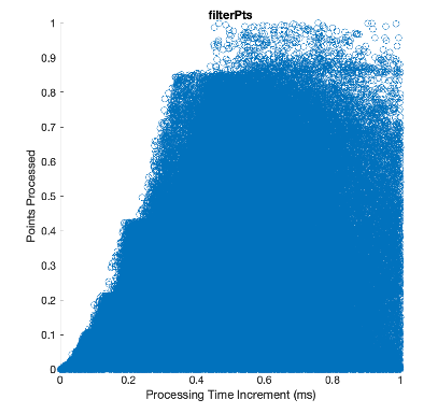
\includegraphics[width=\textwidth]{Images/gbcache/filter_points_scatter.png}
        \caption{Scatter plot of duration of \texttt{filter\_points} against number of LiDAR points}
        \label{fig:gbcache_filter_points_scatter}
    \end{subfigure}
    \hspace{2em} % horizontal spacing between them
    \begin{subfigure}[t]{0.44\textwidth}
        \centering
        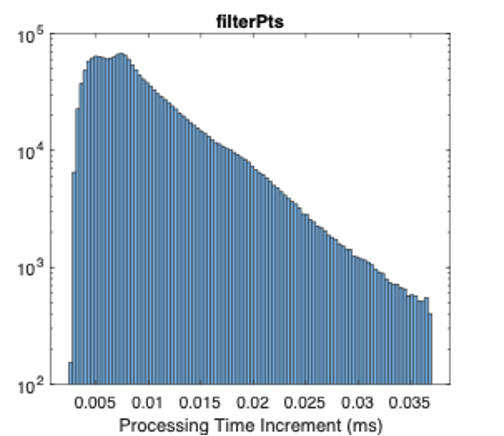
\includegraphics[width=\textwidth]{Images/gbcache/filter_points_hist.png}
        \caption{Histogram of duration of \texttt{filter\_points} against number of LiDAR points}
        \label{fig:gbcache_filter_points_hist}
    \end{subfigure}
}
\caption{Scatter (a) and histogram (b) plots of \texttt{filter\_points} process plotted against number of LiDAR points}
\label{fig:gbcache_filter_points}
\end{figure}

\begin{figure}[htbp]
\centering
\makebox[\textwidth][c]{
    \begin{subfigure}[t]{0.44\textwidth}
        \centering
        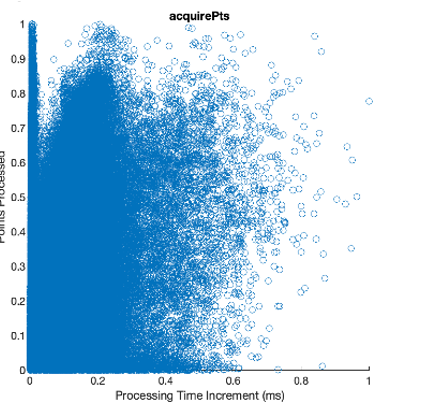
\includegraphics[width=\textwidth]{Images/gbcache/Add_points_scatter.png}
        \caption{Scatter plot of duration of \texttt{add\_points} against number of LiDAR points}
        \label{fig:gbcache_add_points_scatter}
    \end{subfigure}
    \hspace{2em} % horizontal spacing between them
    \begin{subfigure}[t]{0.44\textwidth}
        \centering
        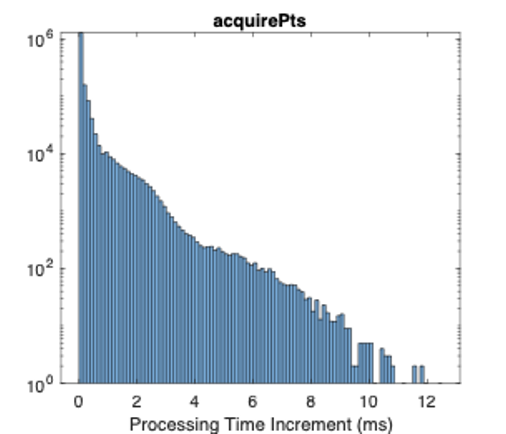
\includegraphics[width=\textwidth]{Images/gbcache/Add_points_hist.png}
        \caption{Histogram of duration of \texttt{add\_points} against number of LiDAR points}
        \label{fig:gbcache_add_points_hist}
    \end{subfigure}
}
\caption{Scatter (a) and histogram (b) plots of \texttt{add\_points} process plotted against number of LiDAR points}
\label{fig:gbcache_add_points}
\end{figure}

\begin{figure}[htbp]
    \centering
    % Subfigure (a)
    \begin{subfigure}[b]{0.44\linewidth}
        \centering
        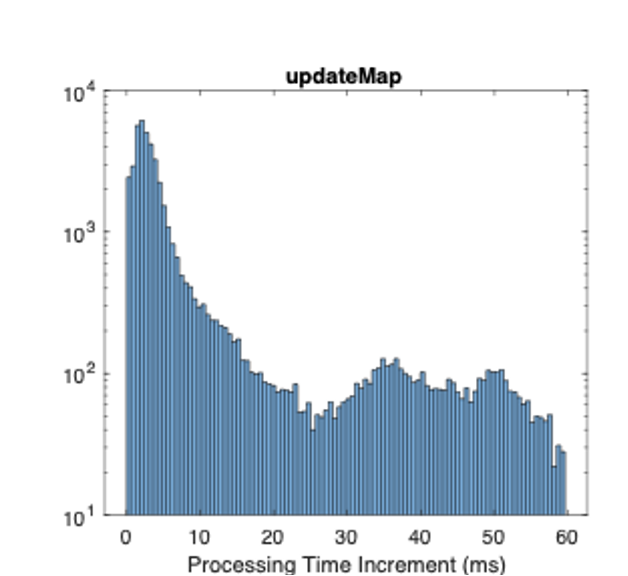
\includegraphics[width=\linewidth]{Images/gbcache/Update_Map_hist.png}
        \caption{Histogram of duration of \texttt{map\_update} against number of LiDAR points}
        \label{fig:gbcache_update_map_hist}
    \end{subfigure}
    \vspace{1em} % vertical spacing between subfigures
    % Subfigure (b)
    \begin{subfigure}[b]{0.8\linewidth}
        \centering
        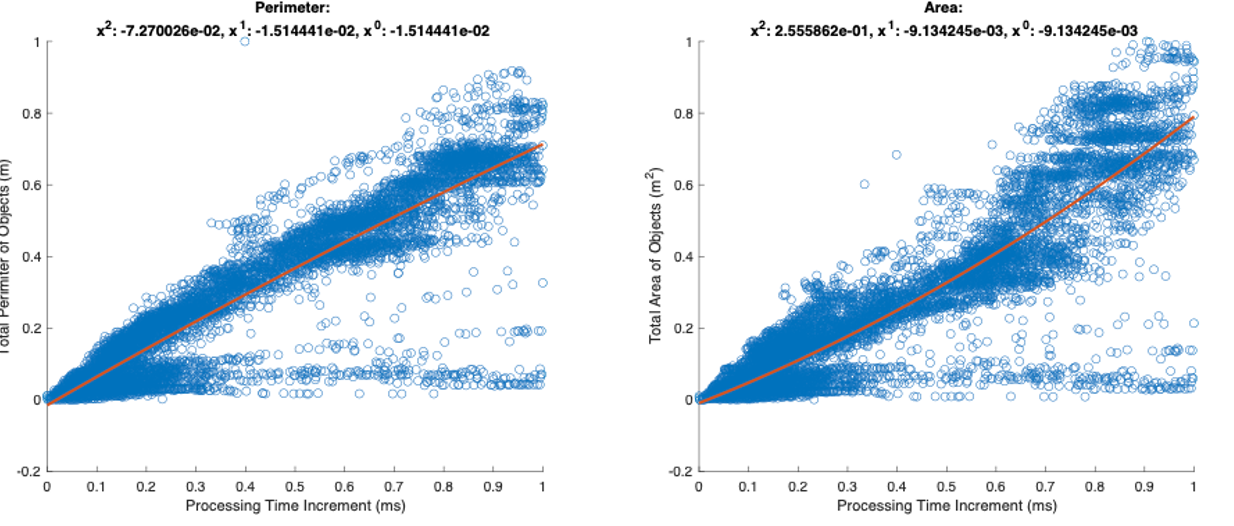
\includegraphics[width=\linewidth]{Images/gbcache/Update_Map_scatter.png}
        \caption{Two scatter plot of duration of \texttt{map\_update} against average perimeter length of polygon (left), and against average area of polygon (right). The line of best-fit is shown in red for each, with associated polynomial values of: $x^2 = -0.0727, x^1 = -0.0151, x^0 = -0.0151$ (left) and $x^2 = 0.2556, x^1 = -0.00913, x^0 = -0.00913$ (right) }
        \label{fig:gbcache_update_map_scatter}
    \end{subfigure}

    \caption{Histogram (a) and scatter (b) plots of \texttt{map\_update} process plotted against number of LiDAR points}
    \label{fig:gbcache_update_map}
\end{figure}




%%%%%%%%%%%%%%%%%%%%%%%%%%%%%%%%%%%%%%%%%%%%%%%%%%%%%%%%%%%%%%%%%%%%
%%%%%%%%%%%%%%%%%%%%%%%%%%%%%%%%%%%%%%%%%%%%%%%%%%%%%%%%%%%%%%%%%%%%
%%%%%%%%%%%%%%%%%%%%%%%%%%%%%%%%%%%%%%%%%%%%%%%%%%%%%%%%%%%%%%%%%%%%
\chapter{Late Fusion} \label{late_fusion}

\chapter{Conclusions} 

% This chapter will synthesize findings from all three research objectives:
% - Summary of comparative performance results between LiDAR and vision systems
% - Calibration and synchronization framework effectiveness
% - Real-time processing capability validation
% - Implications for ASV perception system design
% - Contribution to maritime autonomous systems knowledge

\section{Research Objective Achievement Summary}
% Placeholder for objective completion summary

\section{Performance Comparison Findings}
% Placeholder for key comparative analysis conclusions

\section{Implications for ASV System Design}
% Placeholder for practical design guidance conclusions

\chapter{Recommendations and Future Work} 

\section{recommendations} \label{reccomendations}

\section{Future Work} \label{futurework}

This dual-system configuration facilitated the transition of Minion's software during the period of this research.
\ac{ROS} 1 was the operational framework for all research and data collected in this study, however, \ac{ROS} 1 has entered end-of-life for active development.
Consequently, Minion’s software architecture was gradually migrated to \ac{ROS} 2, which introduces substantial improvements in real-time performance, memory management, and inter-process communication.
In contrast to ROS 1’s reliance on a centralized message broker, ROS 2 employs a Data Distribution Service-based communication layer that reduces latency and memory overhead through zero-copy data handling and improved resource allocation.
Maintaining one system on ROS 1 while transitioning the other to ROS 2 allowed incremental software migration without interrupting field operations—laying the groundwork for future runtime performance improvements anticipated in Section~\ref{futurework}.

% This chapter will address:
% - Recommendations for ASV perception system design based on findings
% - Sensor selection guidance for maritime applications
% - Future research directions for maritime sensor fusion
% - Technology transfer opportunities to operational systems

\section{ASV Perception System Design Recommendations}
% Placeholder for design guidance recommendations

\section{Future Research Directions}
% Placeholder for future work recommendations

\section{Technology Transfer Opportunities}
% Placeholder for practical application recommendations




% \printbibliography
% \bibliographystyle{plainnat} - Most recent
\bibliographystyle{IEEEtranN} % natbib-compatible numeric IEEE style
% \bibliography{References}
\bibliography{Dissertation}

\backmatter

\chapter{Image Transform} \label{img_tform}

To obtain the two-dimensional pixel coordinates of the distorted image ($u, v$) in the camera frame $C$ from a three-dimensional coordinate ($X_{L}, Y_L, Z_L$) in the LiDAR frame $L$:

% 3D LiDAR point to distorted image pixel
% \paragraph{Projection from LiDAR to image.}
Let $\mathbf{R}\in \mathbb{R}^{3\times3}$, $\mathbf{t}\in \mathbb{R}^{3\times1}$, $_L\mathbf{P} = [X_L, Y_L, Z_L, 1]^T$,  and $_C\mathbf{P} = \;_{C}^{L}\mathbf{T} \; _L\mathbf{P}$, then:
\begin{equation*}
_C\mathbf{P} = [X_C, Y_C, Z_C, 1]^T \;= \; _{C}^{L}\mathbf{T} \;[X_L, Y_L, Z_L, 1]^T,
% ,\qquad
% _{C}^{L}\mathbf{T} =
% \begin{bmatrix}
% \mathbf{R}_{C}^{L} & \mathbf{t}_{C}^{L} \\
% \mathbf{0}^T & 1
% \end{bmatrix}.
% \label{eq:LiDAR_to_cam_frame}
\end{equation*}

such that:
\begin{equation*}
    _{L}^{C}\mathbf{T} =
    \begin{bmatrix}
        _{L}^{C}\mathbf{R} & _{L}^{C}\mathbf{t} \\
        \mathbf{0}^\mathrm{T} & 1
    \end{bmatrix},
\end{equation*}

We obtain the pixel coordinates ($x_n, y_n$) in the undistorted image frame by pinhole projection:
\begin{equation*}
x_n = \frac{X_C}{Z_C}, \qquad
y_n = \frac{Y_C}{Z_C}, \qquad
r^2 = x_n^2 + y_n^2 .
\label{eq:normalized_coords}
\end{equation*}

Apply the radial distortion model:
\begin{align*}
r^2 & = x_n^2 + y_n^2 .\\
x' & = x_n\!\left(1 + k_1 r^2 + k_2 r^4 + k_3 r^6\right), \\
y' & = y_n\!\left(1 + k_1 r^2 + k_2 r^4 + k_3 r^6\right).
\label{eq:radial_distortion_apply}
\end{align*}

Map ($x', y'$) to distorted pixel coordinates ($u,v$) using the intrinsic matrix $\mathbf{K}$:
\begin{equation}
\begin{bmatrix} u \\ v \\ 1 \end{bmatrix}
=
\begin{bmatrix}
f_x & s & c_x \\
0   & f_y & c_y \\
0   & 0   & 1
\end{bmatrix}
\begin{bmatrix} x' \\ y' \\ 1 \end{bmatrix},
\qquad
% \mathbf{K} =
% \begin{bmatrix}
% f_x & s & c_x \\
% 0   & f_y & c_y \\
% 0   & 0   & 1
% \end{bmatrix},
% \quad
\Rightarrow\ 
\begin{cases}
u = f_x x' + s y' + c_x,\\
v = f_y y' + c_y.
\end{cases}
\label{eq:intrinsics_to_pixels}
\end{equation}
\chapter{test 2}

% Tables of Results

% \chapter{Another Test of the Appendix System}
% Supplemental Figures.
\end{document}

